\documentclass[10pt,a4paper]{article}
\usepackage[utf8]{inputenc}
\usepackage[T1]{fontenc}
\usepackage[italian]{babel}
\usepackage[a4paper,top=2cm,bottom=3cm,left=3.2cm,right=3.2cm,bindingoffset=0mm]{geometry}
\usepackage{amsmath}
\usepackage{amsfonts}
\usepackage{amssymb}
\usepackage{makeidx}
\usepackage{placeins}
\usepackage{graphicx}
\newtheorem{theorem}{Theorem}
\newtheorem{exercise}{Exercise}
\newtheorem{example}{Example}
\newtheorem{corollary}{Corollary}[theorem]
\newtheorem{lemma}[theorem]{Lemma}
\newtheorem{definition}{Definition}
\newtheorem{prop}{Proposition}
\makeatletter
\def\th@plain{%
	\thm@notefont{}% same as heading font
	\itshape % body font
}
\def\th@definition{%
	\thm@notefont{}% same as heading font
	\normalfont % body font
}
\newcommand{\newparallel}{\mathrel{\mathpalette\new@parallel\relax}}
\newcommand{\new@parallel}[2]{%
	\begingroup
	\sbox\z@{$#1T$}
	\resizebox{!}{\ht\z@}{\raisebox{\depth}{$\m@th#1/\mkern-5mu/$}}%
	\endgroup
}
\makeatother
\author{Fabio Prestipino}
\title{Fenomeni termici}

\begin{document}
\maketitle

\section{Introduzione}
	Possiamo vedere la Termodinamica come una generalizzazione e reinterpretazione della meccanica classica, con un aggiunta di nuovi concetti. Einstein sostenne che la termodinamica è immortale perché non sostituibile o ampliabile (nel suo ambito di competenza). A Differenza della meccanica classica, la termodinamica permette di studiare qualsiasi sistema fisico. Questa nuova branca della fisica venne sviluppata nella seconda metà del XIX secolo, duecento anni dopo la nascita della scienza moderna, principalmente dalle celeberrime figure di Carnot, Kelvin, Joule, Clausius, Gibbs, Maxwell e Boltzmann (fra molti altri, fra cui alcuni ingegneri). L'approccio, più moderno, risulta differente ed è bene introdurre i termini del problema in una nuova forma.\\
	\subsection{Lo stato di un sistema fisico}
		"Conoscere" un sistema fisico vuol dire conoscere il suo \textbf{stato} in un dato istante o intervallo di tempo.
		Possiamo parlare di \textbf{micro-stato} di un sistema, dato dalla coppia di posizione e quantità di moto di ogni particella che compone il sistema ad un dato istante. 
		\begin{align*} 
			\text{Micro-stato del sistema } = \{ \vec{x}_i,\ \vec{p}_i\}
		\end{align*} 
		Esiste inoltre il macro-stato di un sistema, ovvero la coppia di due coordinate specifiche (macroscopiche) del sistema dette \textbf{coordinate termodinamiche}. Un classico esempio è il recipiente cilindrico pieno di gas e messo a pressione da un pistone, questo macro sistema fisico ha come coordinate macroscopiche specifiche pressione e volume dunque il suo stato sarà dato da $\{P,\ V\}$. Fra le coordinate macroscopiche distinguiamo tra \textbf{intensive} ed \textbf{estensive}, le seconde variano con le dimensioni del sistema mentre le prime no. Esiste una relazione interessante fra questi due tipi di coordinate: ognuna di un tipo ha un suo coniugato (\textbf{variabili coniugate}) nell'altro tipo, ad esempio 
		\begin{align*} 
			&(V,\ l ,\ S,\ R,\ H)\\
			&\quad \quad \quad \downarrow\\
			&(P,\ T,\ \tau,\ \epsilon,\ M)
		\end{align*} 
		Questa caratteristica risulterà utile in seguito.\\
		Un insieme di coordinate macroscopiche può essere indipendente o dipendente, nel primo caso le coordinate possono assumere qualsiasi valore indipendentemente dalle altre mentre nel secondo esiste una funzione, che ha come parametri alcune delle coordinate, da cui dipende una delle coordinate restanti (il suo valore non sarà dunque libero). 
		\begin{definition}[Stato termodinamico]
			Si dice stato termodinamico (macroscopico) di un sistema i valori che assumono un'insieme di coordinate termodinamiche indipendenti di un sistema in un dato istante. Differisce dallo stato meccanico (microscopico) di un sistema definito dai valori dalle coordinate di posizione e quantità di moto di un sistema in un dato istante. 
		\end{definition}
		Risulta chiaro che dovremo usare approcci diversi a seconda se vorremo "conoscere" il sistema (lo stato) dal punto di vista microscopico o macroscopico: vediamoli. 
	\subsection{Approccio microscopico}	
		Questo approccio applica semplicemente quanto visto in meccanica classica: dato un sistema formato da N punti, mediante le \textbf{equazioni cardinali} possiamo studiare l'evoluzione nel tempo dello stato del sistema conoscendo lo stato del sistema ad un dato istante, che sarà il nostro $t = 0$. Il micro-stato è formato da due grandezze vettoriali, dunque per ognuna delle particelle avremo $3+3$ equazioni, avendo N particelle, per conoscere lo stato del sistema ad un dato istante necessiteremo di $6N$ equazioni. \\
		Nel caso semplice di N = 1, campo di forze costanti e moto unidimensionale lo studio dell'evoluzione dello stato si riduce ad risolvere una semplice equazione differenziale
		\begin{align*} 
			F = m \ddot{x} \Rightarrow 
			\begin{cases}
				x(t) = x_0+v_0 t +\frac{1}{2} \frac{F}{m} t^2\\
				v(t) = v_0 + \frac{F}{m} t
			\end{cases}
		\end{align*} 
		Per rappresentare graficamente la legge oraria possiamo elaborare un grafico orario "x su t" mentre per effettuare un plot dello stato del sistema necessiteremo di un grafico "p su x" (dall'uno è sempre possibile ricavare l'altro in modo semplice), ogni punto rappresenta lo stato ad un dato istante. \\
		Se volessimo generalizzare quanto visto per un sistema di N corpi con un moto in $\Re^3$ ed un campo di forze variabili dovremo risolvere un sistema di N equazioni differenziali 
		\begin{align*} 
			\begin{cases}
				m_1 \ddot{\vec{x}}_1 = \vec{F}_1^{(int)}+\sum \vec{F_1}^{(ext)}\\
				...\\
				m_N \ddot{\vec{x}}_N = \vec{F}_N^{(int)}+\sum \vec{F_N}^{(ext)}
			\end{cases}
		\end{align*} 
		Ad esempio potremmo avere la forza di gravità che agisce come forza esterna su tutto il sistema e le forze elettriche e gravitazionali fra le singole particelle come forze interne. Questo sistema è teoricamente risolvibile (per $N > 2$ si ricorrerà al metodo perturbativo). \\
		Tuttavia, i sistemi fisici macroscopici sono formati da un numero di particelle nell'ordine del numero di Avogadro ($6.022 \cdot  10^{23}$ ) dunque non esisterebbe una potenza di calcolo tale da poter studiare un sistema fisico macroscopico con questo approccio. Nasce allora la necessità di uno studio diverso del sistema.
	\subsection{Approccio macroscopico}
		Possiamo sacrificare la conoscenza degli stati interni del sistema mediante la risoluzione delle equazioni cardinali sfruttando le proprietà del centro di massa, ma è proprio lo stato interno del sistema che interessa la termodinamica. Nasce allora l'esigenza della nascita della \textbf{termodinamica classica} e di quella \textbf{statistica}. La seconda è basata su una visione statistica della meccanica classica, è legittimata dal fatto che i sistemi termodinamici hanno un numero particelle elevatissimo dunque la statistica si applica alla perfezione (con errori trascurabili), tuttavia proprio perchè si basa sulla meccanica classica non è in grado di trattare i fenomeni fuori dal raggio d'azione di quest'ultima. La termodinamica classica invece si basa sulle coordinate macroscopiche specifiche, già viste. 
	\subsection{Diversi tipi di sistemi}
	Possiamo distinguere tre tipi diversi di sistema a seconda degli scambi che questo intrattiene con l'esterno: 
	\begin{itemize}
		\item Aperto : scambia con l'ambiente sia materia che energia;
		\item Chiuso: scambia con l'ambiente solo energia;
		\item Isolato:  non scambia con l'ambiente;
	\end{itemize}
Si noti che in questa sede adottiamo l'assunto della fisica classica per cui materia ed energia sono distinte. A seconda di come si sceglie il sistema, in una stessa situazione potremo avere sistemi di diverso tipo; vediamo un semplice esempio di un caso macroscopico. 
Una massa scivola su una rampa con superficie scabra, parte con velocità nulla da un'altezza h e si ferma arrivata al suolo. Se consideriamo il sistema della massa allora le forze esterne sono la gravità e l'attrito dinamico mentre quelle interne sono di vario tipo ed agiscono fra le particelle della massa. 
\begin{align*} 
	&L= L^{(i)} +  L^{(e)} = \Delta k \quad \text{Teorema delle forze vive}\\
	&mgh - \int_{\Gamma} \mu_D R \hat{u} d\vec{l} - L^{(i)}= 0
\end{align*} 
Se invece il sistema considerato fosse quello della rampa e della massa allora la forza d'attrito sarebbe da considerare interna. La scelta del sistema, come vediamo, è arbitraria e dipende da ciò che si vuole studiare. 
\section{Principio zero e temperatura}
Da ora in poi tratteremo principalmente sistemi macroscopici.\\
Cominciamo con il definire l'\textbf{equilibrio termodinamico}: due o più sistemi si dicono in equilibrio termodinamico se si verificano le tre seguenti condizioni di equilibrio:
\begin{itemize}
	\item Meccanico: nulla si muove ( a livello macroscopico)
	\item Chimico: la composizione e la concentrazione non cambiano nel tempo (quando le componenti chimiche hanno lo stesso potenziale chimico)
	\item Termico: i sistemi hanno la stessa temperatura
\end{itemize}	
Si noti che la temperatura di cui si parla al terzo punto è per noi ancora una grandezza da definire, sappiamo solo che se due sistemi hanno la proprietà di essere all'equilibrio termico, questa grandezza è la stessa per entrambe i sistemi. La termodinamica che studieremo in questa sede si occupa di sistemi all'equilibrio, la trattazione delle fasi di transizione è ben più complessa.\\
Definiamo ora il \textbf{contatto adiabatico} e quello \textbf{termico}: siano due sistemi A e B, di coordinate macroscopiche rispettivamente (x, y) ed (x', y'). Questi sono sono detti in contatto adiabatico se separati da una parete adiabatica, tale che le coordinate non cambino nel tempo; in contatto termico se le coordinate cambiano fino a quando non soddisfano una funzione f(x, y, x', y') = 0. Sia C un terzo sistema fisico di coordinate (x'', y''), disponiamo i sistemi A, B e C in modo che C sia in contatto termico con A e con B ma A sia in contatto adiabatico con B. Ci chiediamo se, in una situazione del genere, dopo un adeguato intervallo di tempo, i due sistemi A e B siano in equilibrio termodinamico fra loro. Questo equivale a chiedersi se vale la proprietà transitiva per l'equilibrio termodinamico. Ciò non è verificabile teoricamente mediante formule e perciò costituisce un principio fondamentale della termodinamica: il \textbf{principio zero}. La risposta è affermativa.
\begin{definition}[Principio zero]
Se un corpo A è in equilibrio termico con un corpo C e anche un altro corpo B è in equilibrio termico con C, allora A e B sono in equilibrio termico tra loro.
\end{definition}
Ne deduciamo che esiste una grandezza che accomuna i sistemi all'equilibrio termico. la temperatura. Scriviamo in formule quanto visto sopra
\begin{align*} 
&\text{A è all'equilibrio termico con C}\\
&f_{AC}(x, y, x'', y'') = 0\\
&\text{B è all'equilibrio termico con C}\\
&f_{BC}(x', y', x'', y'') = 0
\end{align*} 
Sappiamo che le variabili indipendenti sono solamente due, possiamo dunque espirimere una variabile in funzione delle altre, isoliamo quindi in entrambe le equazioni y''. 
\begin{align}\label{eq:temp1}
&\begin{cases}
	y'' = g_{AC}(x, y, x'')\\
	y'' = g_{BC}(x', y', x'')
\end{cases}\\\nonumber
&\Rightarrow g_{AC}(x, y, x'')=  g_{BC}(x', y', x'')
\end{align} 
Esprimiamo ora il prpincipio zero in forma matematica
\begin{align}\label{eq:temp2}
&\text{A è all'equilibrio termico con B}\\ \nonumber
&f_{AB}(x,y, x', y') = 0
\end{align} 
Sappiamo che (\ref{eq:temp1}) e (\ref{eq:temp2}) esprimono lo stesso concetto fisico, deve dunque essere possibile eguagliarle, per farlo dovremo eliminare il termine in x'' della (\ref{eq:temp1}) (che non compare nella (\ref{eq:temp2})). Vista la necessità di poterle eguagliare, la variabile x''  deve essere fattorizzabile (solo così potremmo eliminarlo e dobbiamo poterlo eliminare).
\begin{align*} 
	&g_{AC}(x, y, x'')=h_A(x, y) \Psi(x'') \\
	&g_{BC}(x, y, x'')=h_B(x', y') \Psi(y'')\\
	&h_A(x, y) \Psi(x'')=h_B(x', y') \Psi(y'')\\
	&\Rightarrow h_A(x, y) = h_B(x', y')
\end{align*} 
Quest'ultima equazione deve verificarsi all'equilibrio termico, ciò equivale a dire che devono avere una grandezza comune. La funzione h è chiamata \textbf{isoterma} mentre il valore di h è detto \textbf{temperatura} (che è la grandezza che condividono due sistemi all'equilibrio termico). Possiamo effettuare il plot di tutte le coppie (x, y) che, inserite nell'equazione isoterma $h_A$ risultano nello stesso valore( di temperatura), questo sarà il grafico dell'isoterma. Le isoterme del sistema A e del sistema B, se questi sono all'equilibrio termico, saranno dette \textbf{corrispondenti}. 
\subsection{Termometria}
Ciò che abbiamo fatto fin'ora, è detto termoscopia, ovvero giudicare se due sistemi hanno la stessa temperatura, senza meglio specificare il valore di quest'ultima. Ora invece introduciamo la termometria, cioè la valutazione del valore della temperatura mediante una \textbf{scala termometrica}. \\
Lo scopo che ci proponiamo è di trovare un modo per misurare la temperatura. Sappiamo che per diversi valori di temperatura avremo diverse curve isoterme (infinite, una per ogni valore di temperatura, che è un numero reale), vogliamo trovare una funzione che intersechi tutte le isoterme. Esistono infinite funzioni che soddisfano questa condizione; scegliamo quella più semplice, ovvero quella lineare, con un unica variabile x, assumendo che la y sia la variabile dipendente ed x indipendente (al variare di x la retta interseca diverse isoterme e dunque fornisce diverse temperature).
\begin{align}\label{eq:funztemperatura}
	\theta (x) = a x + b \quad \text{Funzionetemperaturagenerale}
\end{align}  
Per ottenere una scala con la quale misurare la temperatura bisogna determinare i valori dei parametri a e b, essendo due incognite necessiteremo di un sistema a due incognite. 
\begin{align*} 
&\begin{cases}
	&\theta_1 = a x_1 = a x_1 + b\\
	&\theta_2 = a x_2 + b  
\end{cases}\\
&\Rightarrow a = \frac{\theta_1 - \theta_2}{x_1 - x_2}\ ; \quad b = \frac{\theta_2 x_1 - \theta_1 x_2}{x_1 - x_2 }
\end{align*} 
Si noti che $\theta_1$ e $\theta_2$ sono valori arbitrari; nella scala celsius o centigrada, molto diffusa anche nel quotidiano, questi valori sono scelti rispettivamente all'ebollizione e al congelamento dell'acqua a pressione ambientale. Per convenzione (è arbitrario, ed è questo che caratterizza le diverse scale termometriche) diciamo che $\theta_1 = 100$ e $\theta_2 = 0$ sono rispettivamente la temperatura dell'acqua che bolle e dell'acqua che congela. Per calibrare un termometro reale, ad esempio quello al mercurio, basato sulla coordinata termodinamica di volume (il mercurio si espande all'aumentare della temperatura), sostituiamo $x \equiv V$ (dunque $X_1=$ volume dell'acqua a 100 gradi ed analogamente per $x_2$) e sostituiamo i valori ottenuti di a e b nella funzione (\ref{eq:funztemperatura}).
\begin{align*} 
	\theta(V) = 100 \cdot \frac{V- V_0}{V_{100}-V_0}
\end{align*} 
Chiaramente al posto del volume potremmo usare qualsiasi altra variabile a patto che vari al variare della temperatura, il procedimento sarebbe lo stesso. Essendo la funzione lineare, possiamo creare una scala in cui l'intervallo fra una tacca e l'altra rimane sempre uguale.\\
La scala centigrada è stata sostituita poiché, quando si adotta la funzione lineare ad una variabile si presuppone che la y (pressione) resti costante e non influisca sulle misure, ciò in realtà non è del tutto vero e c'è il rischio che in misure di precisione ciò introduca un errore sistematico. Bisognava allora trovare un fenomeno (da sostituire ad ebollizione e congelamento dell'acqua) che avvenisse ad una pressione ben precisa in modo da eliminare il problema (il punto d'ebollizione varia sensibilmente a seconda della pressione). Il fenomeno scelto è il \textbf{punto triplo dell'acqua}, in cui questa raggiunge contemporaneamente stato solido liquido e gassoso, ciò avviene alla pressione esatta di $610.6165\ Pa$ e ad una temperatura esatta di $0.01\ C$. Volgiamo inoltre scegliere una funzione che abbia solamente il termine in a (poniamo b = 0), a differenza della scala celsius. Per determinare la a basterà una sola equazione che sarà calcolata al punto triplo dell'acqua, analogamente a prima ci avvaliamo dell'esempio del volume.
\begin{align}\label{eq:Funzionetemperaturakelvin}
	\theta_3 = a V_3 \Rightarrow a = \frac{\theta_3}{V_3} \Rightarrow \theta(V) = \frac{\theta_3}{V_3} V 
\end{align} 
$\theta_3$ è stato scelto (in modo arbitrario) a 273,16 gradi della nuova scala Kelvin in modo che il coefficiente angolare della retta dei gradi centigradi e quella dei kelvin sia lo stesso, per fare che questo si verifichi bisogna porre $\theta_3\equiv 276.16$. Ora, visto che il punto triplo dell'acqua risulta essere, sperimentalmente, a 0.01 \textdegree C, la conversione da gradi kelvin a gradi centigradi risulta immediata: basterà sottrarre 273.15.\\
Si presenta infine un problema, al variare del materiale scelto per misurare il volume al variare della temperatura, non è detto che la relazione rimanga lineare (cosa che non succede infatti). Ne segue che la temperatura, che dovrebbe essere una proprietà generale, varia a seconda del materiale con cui è definita: bisogna scegliere un materiale "privilegiato" per definirla ma quale? Quello adottato, e da cui è stato ricavato il valore di 273,16 in realtà è una pura astrazione e non esiste nella realtà, stiamo parlando del \textbf{gas perfetto}, di cui approfondiremo in seguito (sezione \ref{sec:termometroagasperfetto}).
\subsection{Breve digressione matematica}
Vogliamo studiare la variazione di volume generata dalla variazione infinitesima di pressione e temperatura. Sappiamo che il sistema fisico considerato ha tre coordinate di cui due indipendenti, inoltre esiste una funzione del tipo
\begin{align*} 
	f(p, V, \theta) = 0
\end{align*} 
Possiamo isolare una delle coordinate, il Volume. Il differenziale del volume è dato dalla somma delle variazioni parziali che ha a causa di una variazione infinitesima di volume e una infinitesima di temperatura. 
\begin{align*} 
	&V = V(\theta, p)\\
	&\begin{cases}
		p\rightarrow p + dp\\
		\theta \rightarrow \theta + d\theta
	\end{cases} \Rightarrow V \rightarrow V + dV\\
	&dV = (\frac{\partial V}{\partial \theta})_p d\theta + (\frac{\partial V}{\partial p})_{\theta} dp
\end{align*} 
Un differenziale in matematica è una grandezza arbitrariamente piccola, in fisica tuttavia questa astrazione non ha senso soprattutto dal momento che stiamo considerando un sistema macroscopico e quindi dobbiamo scegliere sistemi abbastanza grandi per non risolvere le  strutture atomiche. Per definizione, in quest'ambito, un volume infinitesimo sarà costituito da un micrometro cubo. Con un semplice calcolo, ad esempio, possiamo ricavare che in questo volume son contenute 30 miliardi di particelle d'acqua, questa quantità è sufficiente per dare una descrizione statistica del sistema? visto che si tratta di un esperimento di conteggio l'incertezza statistica è poissoniana, calcoliamola
\begin{align*} 
	\frac{\sqrt{N}}{N} = \frac{1}{\sqrt{N}} = 6 \cdot 10^{-6}
\end{align*} 
A partire dall'equazione del differenziale del volume possiamo definire due parametri interessanti: il \textbf{coefficiente di dilatazione volumetrica} e quello di \textbf{comprimibilità isoterma}.
\begin{align*} 
	&\alpha \equiv \frac{1}{V}( \frac{\partial V}{\partial \theta})_p\\
	&\beta \equiv \frac{1}{k} \equiv - \frac{1}{V}( \frac{\partial V}{\partial p})_{\theta}
\end{align*} 
Di seguito sono riportati alcuni esempi di coefficienti per diversi materiali. 
\begin{align*} 
	\begin{cases}
		Aria:\ 3.4\cdot10^{-3} K^{-1}\\
		Ghiaccio:\ 3.4\cdot10^{-3} K^{-1}\\
		Vetro:\ 3.4\cdot10^{-3} K^{-1}
	\end{cases} \quad
	\begin{cases}
		Acqua:\ 4.54\cdot 10^{-7} Pa^{-1}\\
		Aria:\ 10^{-5} Pa^{-1}\\
		Diamante:\ 2.5 \cdot 10^{-9} Pa^{-1}
	\end{cases}
\end{align*} 
Si noti che il vetro ha costante negativa perché presenta la particolare caratteristica di contrarsi all'aumentare della temperatura (in seguito vedremo il perchè)
Se fossimo invece interessati ad una sola dimensione (ad esempio in un filo di rame in cui lunghezza>>raggio) avremo a che fare con dilatazioni lineari
\begin{align*} 
	f(\tau, L, \theta) = 0 \Rightarrow \alpha_L = \frac{1}{L}(\frac{\partial L}{\partial \theta})_{\tau}
\end{align*} 
Dimostriamo ora che per piccole variazioni di temperatura $\alpha = \alpha_L$
\begin{align*} 
	&\alpha \equiv \frac{1}{V} (\frac{\partial V}{\partial \theta})_p \rightarrow V' = V(1 + \alpha \Delta \theta)\\
	&\alpha_L = \frac{1}{L}(\frac{\partial L}{\partial \theta})_{\tau} \rightarrow L' = L(1 + \alpha_L \Delta \theta)\\
	&L'^{3} = L^3 (1 + \alpha_L \Delta \theta)^3 \simeq L^3 (1+3\alpha_L \Delta \theta)\\
	&V' = L'^3 \Rightarrow V' \simeq V (1 + 3 \alpha_L \Delta \theta)\\
	&\alpha = 3\alpha_L
\end{align*} 
Visto che l'approssimazione fatta si basa sull'approssimazione al primo termine della serie di Taylor, la sua validità è ristretta a piccole variazioni di temperatura.\\
\begin{exercise}
Si consideri un grande recipiente contenente mercurio liquido, un cubo di lato l fatto d'acciaio galleggia e la parte immersa misura d; dopo una variazione di temperatura $\Delta \theta$ entrambi i materiali si dilatano, in modo diverso: il cubo d'acciaio sprofonderà di più (d' > d) ? L'espansione avviene a pressione costante (quella atmosferica) dunque useremo il coefficiente di dilatazione volumetrica ($\alpha_a$ per l'acciaio e $\alpha_m$ per il mercurio). Il problema ci fornisce il coefficiente di dilatazione lineare dell'acciaio ($\alpha_a$) e quello di dilatazione volumetrica del mercurio ($\beta_m$). Indichiamo inoltre le densità con $\rho_a$ e $\rho_m$.
\begin{align*} 
	&\alpha_a = 1.2 \cdot 10^{-5} °C^{-1}\\
	&\beta_m = 1.8 \cdot 10^{-1} °C^{-1}\\
	&\rho_a l^3 = \rho_m l^2 d \Rightarrow d = \frac{\rho_a}{\rho_m} l\\
	&\rho'_a l^3 = \rho'_m l'^2 d' \Rightarrow d' = \frac{\rho_a'}{\rho_m'} l'\\
	&\begin{cases}
		l' = l (1 + \alpha_a \Delta \theta)\\
		\rho_m' = \frac{m }{V'_m} = \frac{m}{V (1 + \beta_m \Delta \theta)} = \rho_m (1 + \beta_m \Delta \theta)^{-1}\\
		\rho_a' = \frac{m }{V'_a} = \frac{m}{l^3 (1 + \alpha_a \Delta \theta)^3} = \rho_a (1 + \alpha_a \Delta \theta)^{-1}\\
	\end{cases}\\
	\Rightarrow d' &= \frac{\rho_a'}{\rho_m'} l' = \frac{\rho_a (1 + \alpha_a \Delta \theta)^{-1}}{\rho_m (1 + \beta_m \Delta \theta)^{-1}} l (1 + \alpha_a \Delta \theta)\\
	&d \frac{(1 + \beta_m \Delta \theta)}{(1 + \alpha_a \Delta \theta)^2}\simeq d \frac{(1 + \beta_m  \Delta \theta)}{1+2 \alpha_a \Delta \theta}
\end{align*}  
Dove per l'approssimazione ci siamo sempre avvalsi della serie di Taylor. Notiamo che la frazione che moltiplica d è maggiore di uno se sostituiamo le quantità fornite dal problema, ne deduciamo che $d' > d$ e che quindi il cubo d'acciaio sprofonda ulteriormente. 
\end{exercise} 
\subsection{Dilatazione dal punto di vista microscopico}
Fin ora abbiamo visto, dal punto di vista macroscopico, che se aumentiamo la temperatura i corpi di solito si dilatano ed in qualche caso particolare si contraggono, di ciò facciamo esperienza anche nel quotidiano. Tuttavia, se la temperatura è una grandezza emergente dal microscopico, perché una sua variazione ha effetto sulle dimensioni dei materiali?\\
Esiste un modello empirico detto di Lennard-Jones che elabora una funzione di potenziale per le forze agenti fra molecole (che dipende dalla distanza a cui si trovano le molecole). 
\begin{align*} 
	U(r) = \varepsilon[(\frac{r_{min}}{r})^{12}-2(\frac{r_{min}}{r})^6]
\end{align*} 
\begin{figure}[h!]
	\centering
	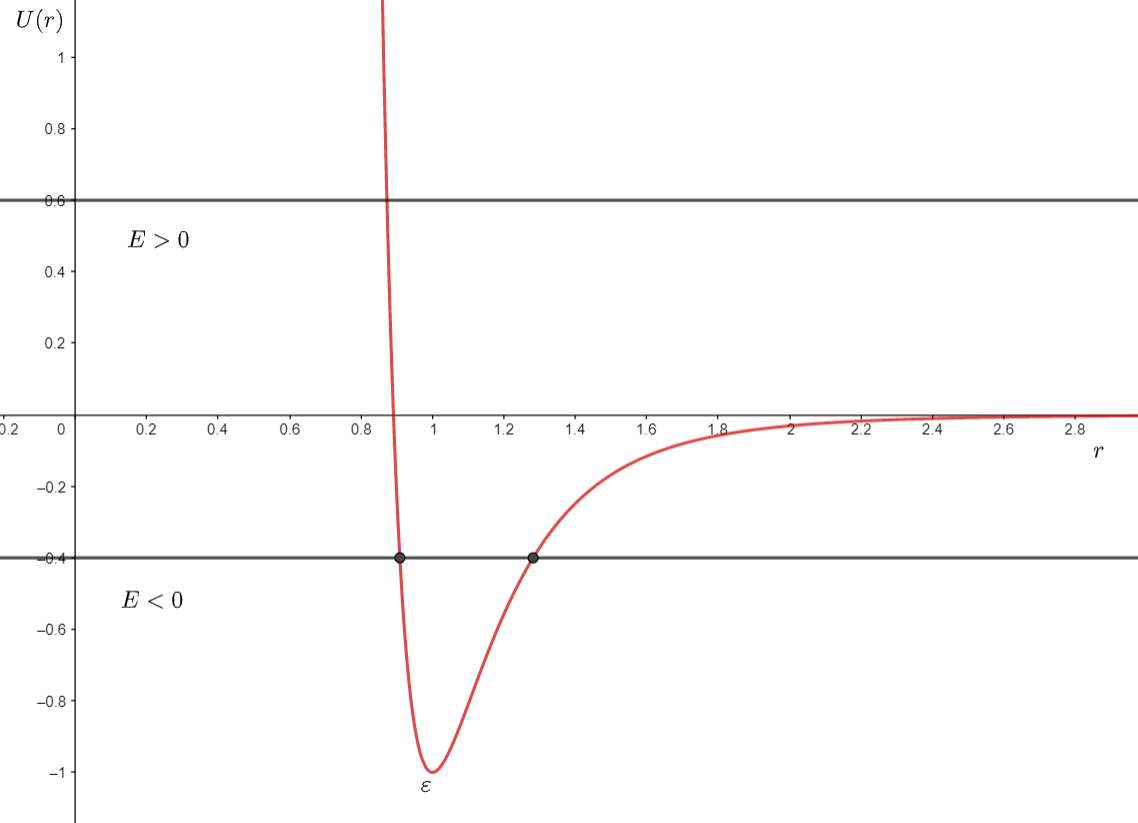
\includegraphics[width=0.6\linewidth]{../images/../images/Lennard-Jones_model}
	\caption{Grafico del potenziale con $\varepsilon =r_min = 1$.}
	\label{fig:lennard-jonesmodel}
\end{figure}
\FloatBarrier
Nell'interazione fra particelle di un gas entrano in gioco una forza repulsiva molto forte $((\frac{r_{min}}{r})^{12})$, che però si attiva a brevi distanze, dovuta alla repulsione elettrostatica di cariche dello stesso segno, e da una forza attrattiva $(-\frac{r_{min}}{r})^6)$ che prevale per le distanze maggiori e che tende a zero per distanze infinite. La curva di potenziale di Lennard-Jones è asimmetrica in quanto per piccole distanze si verifica un muro di potenziale mentre per lunghe distanze va a zero lentamente. All'aumentare dell'energia interna del sistema (che a livello macroscopico è la temperatura) l'ampiezza delle oscillazioni ($r_min$) intorno al punto medio aumenta.\\
Ad una temperatura e volume iniziali, un gas avrà un punto medio stabile attorno al quale avvengono le oscillazioni delle particelle e che a livello macroscopico è rispecchiato dalla costanza del volume del gas (ad una stessa pressione e temperatura). Se si aumenta la temperatura, a causa dell'asimmetria della curva, anche il punto medio tende a spostarsi verso destra, ciò si riflette in un aumento di volume. Ora che il concetto di espansione, pressione e temperatura sono più chiari possiamo definire il concetto di trasformazione termodinamica
\begin{definition}
	Si dice trasformazione termodinamica un processo che connette stati termodinamici all'equilibrio
\end{definition}
\subsection{Il termometro a gas perfetto}\label{sec:termometroagasperfetto}
In fisica una grandezza deve poter essere misurata in modo univoco e preciso, è dunque necessario creare uno strumento per la misura della temperatura, il termometro, in modo ottimale. Abbiamo già osservato che diversi materiali hanno diverse espansioni a parità di variazione di temperatura (infatti ogni materiale ha uno specifico coefficiente d'espansione isoterma), questo costituisce un problema per la misura; vediamo come ovviarlo.\\
Cominciamo a costruire un termometro che adotti un qualsiasi tipo di gas, ad esempio n moli di $O_2$, e che effettui la misura di temperatura sfruttando la pressione come variabile termometrica.
\begin{figure}[h!]
	\centering
	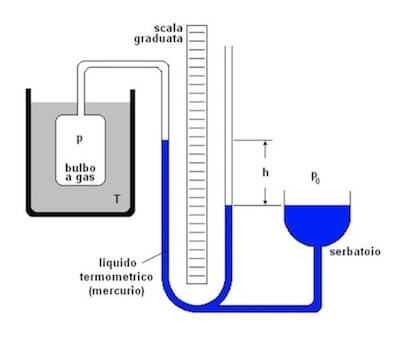
\includegraphics[width=0.6\linewidth]{../images/termometro-a-gas}
	\caption{Schematizzazione del termometro a gas}
	\label{fig:termometro-a-gas}
\end{figure}
\FloatBarrier
Come vediamo in figura, lo strumento è costituito da un bulbo pieno di gas da cui si diparte un tubo pieno di mercurio (gas e mercurio stanno a contatto), abbiamo poi un serbatoio mobile (solamente basso-alto). Sia $p_0$ la pressione atmosferica e $p_3$ quella al punto triplo del gas e $\rho$ la densità del mercurio. La pressione che agisce sul gas (p) è data dalla pressione atmosferica più la pressione della colonna di mercurio (alta h)
\begin{align*} 
	p = p_0 + \rho g
\end{align*} 
Quest'ultima è la \textbf{legge di Stevino}, che viene meglio spiegata nella (\ref{eq:stevin}).\\
Vogliamo ora misurare, ad esempio, la temperatura dell'acqua in ebollizione, volendo adottare la pressione come variabile termometrica bisogna mantenere il volume costante (trasformazione isocora) e misurare la variazione di pressione in ragione della temperatura. Seguiamo i seguenti step:
\begin{enumerate}
	\item Taratura: si immerge il termometro in una cella a punto triplo e si misura la pressione $p_3$, ovvero la pressione del gas portato alla temperatura del punto triplo dell'acqua. 
	\item Successivamente si mette a contatto il termometro col corpo da misurare (in questo caso si immerge il bulbo in acqua bollente), e si misura la nuova pressione p analogamente a quanto fatto per la pressione $p_3$. Attenzione: in questa operazione, il volume del gas deve ovviamente rimanere costante, e a tale scopo agiamo sul manometro indicato in figura: esso sfrutta le proprietà dei vasi comunicanti per far tornare il volume del gas a quello iniziale (a $p_3$).
	\item Si calcola la temperatura del gas usando la relazione (\ref{eq:Funzionetemperaturakelvin}) con p al posto di V: $\theta = \frac{p}{p_3} \cdot 273.16 K$ (in questo caso $\theta(p) = 373.15$).
\end{enumerate}
Possiamo ripetere queste procedure diminuendo progressivamente le moli di gas nel bulbo, per ogni iterazione si registrano i nuovi valori $p’$, $p_3’$ che sono una funzione del numero di moli di gas presenti nel bulbo. Ne risulta che i valori di temperatura $\theta$ sono tutti diversi fra loro e decrescenti al diminuire delle moli, si dispongono su una retta. Se poi ripetiamo la stessa procedura per diversi materiali, otterremo tante rette differenti, come riportato nel seguente grafico
\begin{figure}[h!]
	\centering
	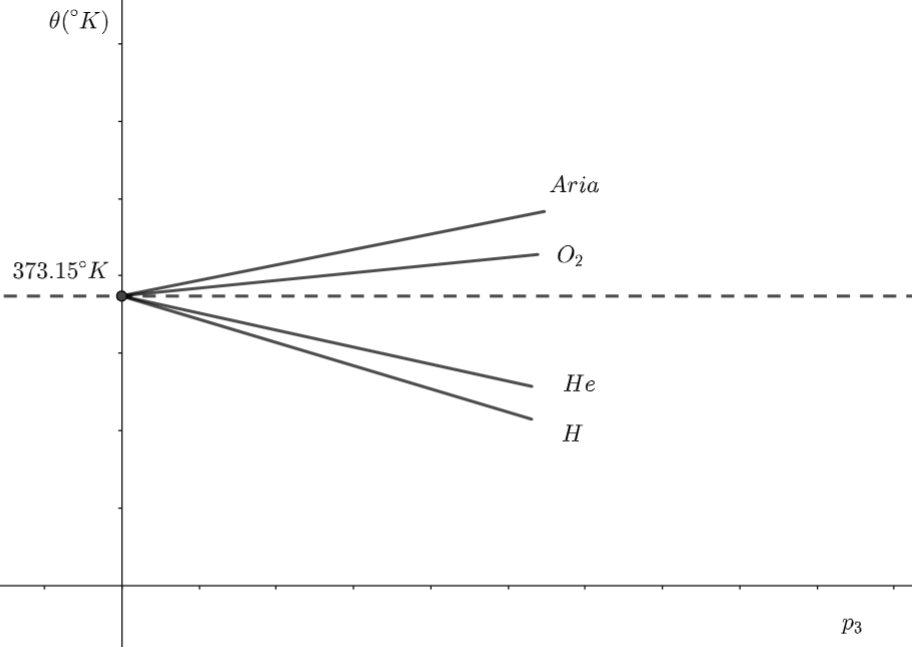
\includegraphics[width=0.6\linewidth]{../images/temp_e_puntotriplo}
	\caption{Esempi di rette ($\theta$, $p_3$) per aria, ossigeno, elio e idrogeno}
	\label{fig:tempepuntotriplo}
\end{figure}
\FloatBarrier
Alcune domande sorgono spontanee:
\begin{itemize}
 \item Perché elio e idrogeno hanno pendenza negativa mentre tutti gli altri gas positiva?\\
 
 \item Perché tutti i gas, basandosi sulla retta di regressione lineare (nel grafico), nonostante abbiano espansioni diverse, per $\lim_{n \to 0}$ misurano tutti la stessa temperatura (che è proprio quella che ci aspettavamo, 100\textdegree C)? \\
   Se le particelle di un gas sono estremamente lontane fra loro ($n \to 0$) non esercitano nessuna interazione reciproca, in questa situazione i gas non presentano differenze fra loro, la temperatura dipenderà unicamente dal movimento delle particelle di gas (energia cinetica media del gas), approfondiremo questo concetto nella sezione (\ref{sec:teoriacinetica}). Se un gas è sufficientemente rarefatto e il volume delle singole particelle è abbastanza piccolo, saremo nelle condizioni di un \textbf{gas perfetto}. Questa è chiaramente una astrazione matematica poiché è impossibile ridurre esattamente a zero le interazioni ma esistono casi, ad esempio quello dell'aria nell'atmosfera, che approssimano molto bene queste condizioni. Per ogni elemento nelle condizioni di gas perfetto l'acqua in ebollizione ha la stessa temperatura: 373.15 \textdegree K.
  \item Perché diminuendo le moli di gas nel bulbo diminuisce anche la misura di temperatura (che ci aspettiamo essere 100\textdegree C = 373.15 \textdegree K e invece risulta sempre maggiore negli esperimenti)? 
   Man mano che si diminuiscono le moli ci si avvicina sempre di più alla condizione di gas perfetto. In altre parole la misura di temperatura diventa sempre più una misura di energia cinetica e tiene conto sempre meno dell'energia intermolecolare (che invece aumenta all'aumentare delle moli, secondo il grafico di Lennard-Jones).
\end{itemize}
In conclusione, esiste una tabella di punti fissi (come il punto triplo dell'acqua) utile per la taratura di termometri utili a misurazioni in qualsiasi range di temperatura:
\begin{figure}[h!]
	\centering
	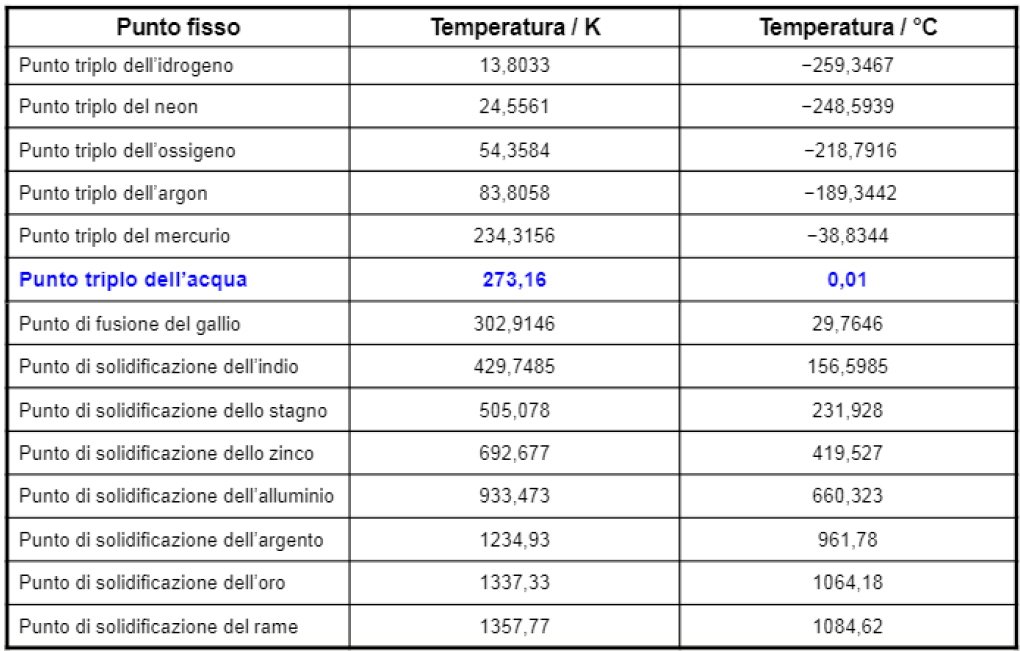
\includegraphics[width=0.7\linewidth]{../images/Punti_fissi}
	\caption{Tabella dei principali punti fissi utili per la taratura di termometri}
	\label{fig:puntifissi}
\end{figure}
\FloatBarrier
Per ora, la misura di temperatura è ancora strettamente legata alla variazione di volume dei gas, tuttavia sappiamo che a basse temperature i gas cambiano stato liquefacendosi. Il gas che ha temperatura di liquefazione minore è l'elio che cambia di stato intorno a 0.5 \textdegree K, più in basso di questa temperatura non è possibile sfruttare un termometro a gas per effettuare misure e, visto che in fisica una grandezza ha senso solo se è misurabile, per ora la temperatura è definita a partire dai 0.5 gradi Kelvin. Vedremo che sarà possibile effettuare misure di temperatura anche molto minori quando svincoleremo il concetto di temperatura dalla sostanza termometrica usata per la misura, in quel momento, effettueremo il passaggio dalla simbologia usata fin' ora, $\theta$ (misurata col termometro a gas perfetto), al conosciuto simbolo $T$ (temperatura termodinamica assoluta).\\
Possiamo dunque dare una prima definizione di temperatura
\begin{definition}[Temperatura termometrica]
	Si dice temperatura termometrica di un sistema fisico (indicata con $\theta$) la quantità misurata mediante un termometro a gas perfetto.
\end{definition}

\section{Gas Perfetti}
Possiamo dare una definizione precisa del nuovo concetto appena visto di gas perfetto
\begin{definition}
Un gas si dice \textbf{perfetto} se valgono contemporaneamente le due seguenti condizioni
\begin{itemize}
\item Il volume delle molecole è trascurabile rispetto a quello del contenitore.
\item Le interazioni intermolecolari a lungo raggio sono trascurabili (le molecole sono sufficientemente distanti fra loro). 
\end{itemize}
\end{definition}
A partire da esperimenti si è arrivati nel tempo (prima metà del 1800) alla formulazione di quattro leggi empiriche ($\beta = \frac{1}{273.15 °C^{-1}}$)
\begin{enumerate}
\item I legge di Gay-Lussacc: a pressione costante
 \begin{align*} 
 &V = V_0 \beta \theta
\end{align*} 
\item II legge di Gay-Lussacc: a volume costante
\begin{align*} 
	p = p_0 \beta \theta
\end{align*} 
\item Legge di Boyle: a numero di moli e temperatura costanti
\begin{align*} 
 V = \frac{cost}{p}
\end{align*} 
\item Legge di Avogadro: a pressione e temperatura costanti
\begin{align*} 
	V = cost' n
\end{align*} 
\end{enumerate}
Dove le temperature sono espresse in Kelvin e $V_0$ e $p_0$ sono volume e pressione del gas perfetto alla temperatura di congelamento dell'acqua (373.15\textdegree K). Questi risultati sono riassunti dalla legge di stato dei gas
\begin{align}\label{eq:gaseperfetti}
	pV = nR\theta
\end{align} 
dove la temperatura è misurata in Kelvin e la costante $R\simeq 8.3145\ mol^{-1}\ K^{-1}$. In condizioni normali (0 oC e 1 atm) tutti i gas (perfetti) occupano lo stesso volume (n = 1 mol), calcolabile con al precedente relazione:
\begin{align*} 
V_0 = \frac{n R \theta}{p_0} = \frac{8.3154\cdot 273.15}{1.013\cdot 10^{5}}\simeq 22.4 l = 0.0224 m^3
\end{align*} 
\begin{exercise}
Trovare i coefficienti di dilatazione termica e di comprimibilità isoterma per un gas perfetto
\begin{align*} 
	\alpha \equiv \frac{1}{V}\frac{\partial}{\partial\theta}_p(\frac{n R \theta}{p}) = \frac{1}{V}\frac{n R}{p}
\end{align*} 
Sostituiamo il volume avvalendoci della (\ref{eq:gaseperfetti})
\begin{align*} 
	&\frac{n R}{n R \theta} = \frac{1}{\theta}\\
	&\frac{1}{k} \equiv -\frac{1}{V}(\frac{\partial V}{\partial p})_{\theta} = -\frac{1}{V}\frac{\partial}{\partial p}(\frac{n R \theta}{p})= \frac{1}{V}\frac{n R \theta}{p^2} = \frac{n R \theta}{(Vp) p} = \frac{n R \theta}{n R \theta p} = \frac{1}{p}
\end{align*} 
\end{exercise} 
\begin{exercise}\label{ex:pressione_quota}
Ricavare la dipendenza della pressione dalla quota atmosferica (assumendo che l’aria sia un gas perfetto).\\
Prendiamo in considerazione un cilindro d'aria di volume V, superficie di base S e altezza dz infinitesima. Sappiamo che la pressione varia con la quota perché più si va in alto minore sarà la forza esercitata dalla colonna d'aria che sovrasta una superficie: la pressione esercitata dall'aria sulla faccia inferiore del cilindro sarà minore (infinitesimamente) di quella sulla faccia superiore. Ricaviamo la relazione che descrive la variazione di pressione in funzione della quota.\\
Se l'aria è ferma in un determinato istante, allora il gas all'interno del nostro cilindro è in equilibrio, cioè la pressione esercitata sulla faccia superiore è uguale e in verso contrario a quella esercitata sulla faccia inferiore più quella esercitata dal gas stesso all'interno del cilindro (i venti sono generati infatti da variazioni di pressione). Dovrà dunque verificarsi
\begin{align}\label{eq:stevin}
	&\text{p faccia superiore} = \text{p faccia inferiore}\\
	&p  = p + dp \nonumber + \frac{(dm) g}{S}\\
	&dp = -\frac{(dm)g}{S} = -\frac{(\rho S dz) g}{S}= -\rho g dz \nonumber \\
	\Rightarrow & \frac{d\rho}{dz}= - \rho g
\end{align} 
Dove p = pressione dell'aria a quota dz
\begin{figure}[h!]
	\centering
	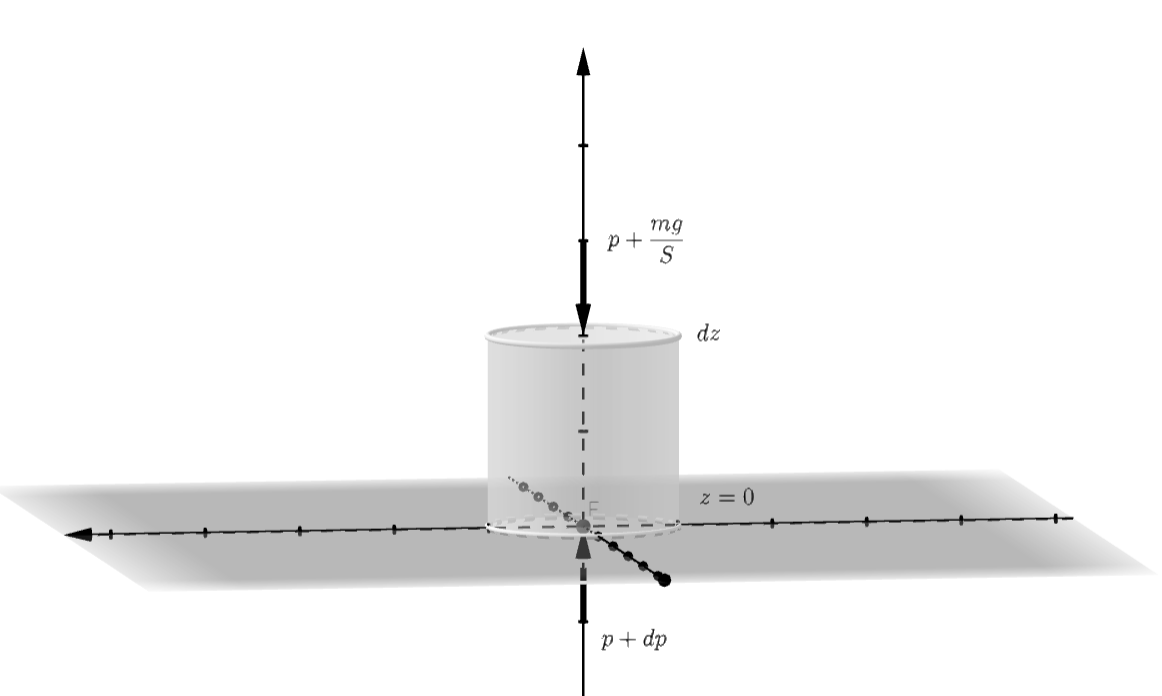
\includegraphics[width=0.5\linewidth]{../images/cilindro_aria}
	\caption{Schema di un cilindro d'aria in equilibrio. La pressione sulle due facce deve uguagliarsi}
	\label{fig:cilindroaria}
\end{figure}
\FloatBarrier
Se la densità dell'aria ($\rho$) fosse costante a qualsiasi quota sarebbe semplice integrare per trovare l'espressione generale della pressione:
\begin{align*} 
	&dp = -\rho  g dz \\
	\Rightarrow & p = p_0 - \rho g z
\end{align*} 
Tuttavia l'aria è un fluido comprimibile, ragion per cui la densità è una funzione della quota ($\rho = \rho(z)$ ). Sfruttiamo le leggi dei gas perfetti per valutare l'espansione dell'aria in funzione della quota (e quindi la sua diminuzione di pressione). Siano m la massa del cilindro pieno d'aria ed M la massa molare dell'aria
\begin{align*} 
	&p V = n R \theta = \frac{m}{M} R \theta \\
	&\rho = \frac{m}{V} = \frac{p V M}{R \theta} \frac{1}{V} = \frac{p M}{R \theta}\\
	&\frac{dp}{dz}=-\rho(z) g = - \frac{p(z) M g(z)}{R\theta(z)}
\end{align*} 
Quest'ultima è la forma generale di come varia la pressione al variare infinitesimo della quota. Si noti che a rigore sia g che $\theta$ dovrebbero variare ma per ora, in prima approssimazione li consideriamo costanti (maggiore precisione sarà aggiunta in seguito). 
\begin{align}\label{eq:esercizio_pressione}
	&\frac{dp}{dz}=- \frac{p(z) M g}{R\theta}\nonumber\\
	&\frac{dp}{p} = -\frac{M g}{R \theta} dz = - L dz
\end{align} 
L'ultimo passaggio è possibile poichè tutti i valori nella frazione sono costanti ($ L \simeq \frac{1}{8.82} km^{-1}$). Integriamo
\begin{align*} 
	&\int_{p_0}^{p} = -L z\\
	& \ln(p) \Big|_{p_0}^p = -L z\\
	&\ln\left(\frac{p(z)}{p_0= - L z}\right)\\
	\Rightarrow& p(z) = p_0 e^{-L z}
\end{align*} 
Se, ad esempio, volessimo sapere a che quota si dimezza la pressione basta fare
\begin{align*} 
	&p(z) = \frac{p_0}{2} \Rightarrow \frac{1}{2} = e^{-L z}\\
	&L z = -\ln(\frac{1}{2}) = \ln(2) \\
	&z = \frac{\ln(2)}{L} \simeq 6100\ m
\end{align*} 
Tale valore sottostima quello reale poiché non abbiamo tenuto conto della diminuzione di temperatura all'aumentare della quota.
\end{exercise}
Prendiamo in considerazione un cilindro con del gas al suo interno ed un pistone che comprime il gas. Vogliamo effettuare una trasformazione di compressione isoterma, che porti da uno stato di equilibrio iniziale A ad uno finale B. Esistono infiniti modi per passare da uno stato all'altro ma se la trasformazione avviene rapidamente allora si creeranno perturbazioni all'interno del cilindro e non tutti i punti del cilindro avranno gli stessi valori di temperatura e pressione. Visto che la pressione è definita come uniforme in tutto il cilindro, se la trasformazione avviene velocemente avremo che negli stati intermedi fra A e B la pressione non sarà definita. Per ovviare a questo problema dobbiamo passare da A a B mediante una trasformazione che comprima il gas in tempi molto lunghi di modo che pressione e temperatura ad un certo istante siano infinitesimamente variati rispetto all'istante precedente. Una trasformazione di questo tipo viene detta \textbf{quasistatica}, un esempio potrebbe essere l'aggiungere un granello di sabbia alla volta sul pistone per aumentare la pressione di un infinitesimo alla volta. 
\begin{definition}
	Una trasformazione quasistatica è una trasformazione termodinamica che avviene in modo estremamente lento, in maniera tale che il sistema in esame, passando da uno stato di equilibrio iniziale A ad uno stato di equilibrio finale B, attraversi una successione di infiniti stati di equilibrio, separati tra loro da trasformazioni infinitesime e da variazioni infinitesime delle proprietà del sistema. Soltanto le trasformazioni quasistatiche possono essere rappresentate come linee continue in un diagramma pressione-volume.
\end{definition} 
La rappresentazione della trasformazione presa in esame si fa su un grafico pressione su volume detto \textbf{piano di Clapeyron}.
\begin{figure}[h!]
	\centering
	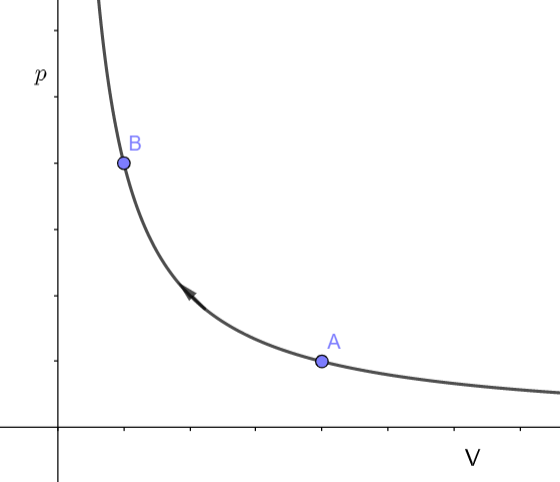
\includegraphics[width=0.5\linewidth]{../images/isoterma}
	\caption{Compressione isoterma rappresentata in un piano di Clapeyron.}
	\label{fig:isoterma}
\end{figure}
\FloatBarrier
 La curva che descrive l'isoterma è un ramo d'iperbole infatti, se la temperatura è costante possiamo scrivere la funzione $p(V)$ come
 \begin{align*} 
 	&p V  = nR\theta \\
 	&p = \frac{n R \theta}{V} = \frac{cost}{V}
 \end{align*} 
Che è proprio la funzione che descrive un'iperbole.
\begin{exercise}
 Un gas si espande come $p(V) = \frac{cost}{V^2}$, $\theta$ aumenta o diminuisce? 
 \begin{align*} 
 	&p V^2 = \left(p V \right) V = cost\\
 	&\left(n R \theta\right) V = cost\\
 	& \theta = \left(\frac{cost}{n R}\right)\frac{1}{V}
 \end{align*}  
Da cui ne segue che le il volume aumenta la temperatura diminuisce.
\end{exercise}
\begin{exercise}
Un sub genera una bolla d'aria sott'acqua, a profondità h, di raggio $r_1 = 2\ mm$. Quando arriva sulla superficie la bolla ha raggio $r_2 = 3\ mm$. Supponendo la temperatura dell'aria all'interno della bolla costante e l'aria un gas perfetto, a che profondità si trova il sub, che pressione c'è a quella profondità?\\
Siano $p_0$ e $V_0$ pressione e volume sulla superficie e $p$ e $V$ a profondità h, possiamo scrivere in entrambi i casi l'equazione di stato dei gas per poi dividere membro a membro e ottenere la pressione a profondità h. 
\begin{align*} 
&\begin{cases}
p_0 V_0 = n R \theta\\
pV = nR\theta
\end{cases}\\
&\frac{p_0 V_0}{p V}=1 \Rightarrow p = \frac{p_0 V_0}{V} = \frac{p_0 \cdot r_2^3}{r_1^3} = p_0 \left(\frac{3}{2}\right)^3 = 341972 Pa
\end{align*} 
Per la legge di Stevino, la pressione a profondità h è uguale alla pressione atmosferica sulla superficie più la pressione generata dalla colonna d'acqua di altezza h sopra il sub. Possiamo eguagliare questa espressione della pressione a quella trovata in precedenza per ricavare h.
\begin{align*} 
&p = p_0 + \rho g h = p_0 \left(\frac{3}{2}\right)^3\\
&h =\frac{p_0}{\rho g} \left(\left(\frac{3}{2}\right)^3 - 1\right) = 24.53\ m 
\end{align*} 
\end{exercise}
\begin{exercise}
Due bulbi sferici di volumi differenti $V_a = 3.18 l$ e $V_b = 1.22 l$ sono collegati da un tubo sottile (volume trascurabile) e hanno un gas perfetto al loro interno. Inizialmente si trovano entrambi a temperatura e pressione iniziale rispettivamente uguali:
\begin{align*} 
&\theta_{ai} = \theta_{bi} = 16 °C\\
&p_{ai} = p_{bi} = 1.44 atm. = 1.44\cdot 1.013 \cdot 10^5\ Pa
\end{align*}  
In seguito si riscalda A fino a portarlo a $\theta_{af} = 108\ °C$ mantenendo $\theta_{bf} = 16\ °C$. Si calcoli la pressione finale del sistema $p_{af}=p_{bf}=p_f$.\\
Osserviamo che se il volume rimane costante e la pressione nei due bulbi è uguale, nonostante la differenza di temperatura, allora si sarà verificato uno spostamento di moli da A a B in modo da bilanciare l'aumento di temperatura con la diminuzione di moli. Possiamo scrivere, essendo il sistema chiuso (non scambia massa con l'esterno)
\begin{align*} 
	n_a + n_b = n_a' + n_b'
\end{align*} 
A partire dall'equazione di stato dei gas isoliamo n e sostituiamo
\begin{align*} 
	&\begin{cases}
	n_a = \frac{p_{ai} V_a}{R \theta_{ai}} \quad n_b = \frac{p_{bi} V_b}{R \theta_{bi}}\\
	n_a' = \frac{p_{af}V_a}{R \theta_{af}} \quad n_b'= \frac{p_{bf}V_b}{R \theta_{bf}}
	\end{cases}\\
	&\frac{p_{ai}V_a}{R \theta_{ai}} + \frac{p_{bi} V_b}{R \theta_{bi}} = \frac{p_{af}V_a}{R \theta_{af}} + \frac{p_{bf}V_b}{R \theta_{bf}}\\
	&p_f = p_0\left[\frac{V_a + V_b}{V_a + \frac{\theta_{bi}}{\theta_{bf}} V_b}\right]
\end{align*} 
\end{exercise}
\section{Gas Reali}
A partire dall'astrazione dei gas perfetti vogliamo trovare un m,odo per descrivere i \textbf{gas reali}. Diamone prima una definizione
\begin{definition}
Un gas è detto \textbf{reale} se vale almeno una delle due seguenti condizioni
\begin{itemize}
\item Il volume delle molecole non è trascurabile rispetto a quello del contenitore. La somma dei volumi delle singole molecole di gas è detto \textbf{covolume}.
\item Le interazioni intermolecolari a lungo raggio non sono trascurabili. 
\end{itemize}
\end{definition}
\begin{definition}
	Il \textbf{covolume} è il limite a cui tende il volume di un gas reale quando la temperatura tende allo zero assoluto (allo zero assoluto le molecole sono massimamente vicine fra loro).
\end{definition}
Per lo studio dei gas reali esistono più approcci, ne vedremo uno efficace dal punto di vista pratico cioè lo \textbf{sviluppo del viriale} ed uno più profondo dal punto di vista teorico che si basa sulla correzione dell'equazione di stato dei gas perfetti. 
\subsection{Sviluppo del viriale}
Definiamo il coefficiente di compressione per i gas reali come
\begin{align*} 
	z_p \equiv \frac{p V}{n R \theta}
\end{align*} 
Può essere definito anche rispetto alla densità come
\begin{align*} 
	z_{\rho} \equiv \frac{p}{R \theta \rho}
\end{align*} 
Se sviluppiamo in serie di Taylor otteniamo
\begin{align*} 
	&z(p) = 1 + Ap + Bp^2+Cp^3+...\\
	&z(\rho)= 1 + A'\rho + B'\rho^2+C'\rho^3+...
\end{align*} 
I parametri A, B, C,... sono misurabili sperimentalmente, variano da gas a gas e anche in base alla temperatura. Sono molto utili a livello pratico e sono tabulati. Come appare chiaro dalla definizione di $z_p$, sarà paria 1 per i gas perfetti e maggiore o minore di uno per i gas reali; possiamo così valutare quanto uno specifico gas ad un valore esatto di pressione e temperatura, si discosti dalle condizioni di gas perfetto. La variazione dal valore ideale di 1 è dovuta dalle interazioni intermolecolari, il fatto che $z_p$ può essere maggiore o minore di 1 è dovuto al fatto che possono verificarsi interazioni attrattive o repulsive. 

\subsection{Correzione dell'equazione dei gas perfetti}
La strategia di questo approccio sta nel modificare la legge di stato dei gas perfetti, aggiungendo due parametri che tengano conto delle due condizioni che differenziano i gas reali dai perfetti: le interazioni intermolecolari ed il covolume. Cominciamo con il chiederci come cambia il volume di un gas reale rispetto ad uno perfetto: il volume di un gas reale sarà sicuramente maggiore di quello di un gas perfetto perché bisognerà tener conto anche del volume delle singole molecole. Ogni mole ha un volume b, il covolume è dato dagli n moli di volume b, dunque
\begin{align*} 
V_{reale} = V_{ideale}+ nb
\end{align*} 
Riflettiamo ora su come cambia la pressione nei gas reali rispetto ai perfetti. A livello microscopico la pressione è data dalle collisioni delle molecole con le pareti del recipiente che contengono il gas, essendo le forze a lungo range di tipo attrattivo queste freneranno le molecole dall'urtare. Ciò provocherà, macroscopicamente, una diminuzione di pressione. Possiamo dunque scrivere
\begin{align*} 
	p_{reale} = p_{ideale} - ?
\end{align*} 
Per ricavare il termine di variazione di pressione prendiamo in considerazione una superficie infinitesima ds del contenitore di un gas ed una molecola che sta per collidere sulla superficie. Se, nel caso di gas perfetto, le interazioni intermolecolari fossero trascurabili, la molecola colliderebbe indisturbata producendo una pressione infinitesima, la somma di tutte le pressioni infinitesime producono la $p_{ideale}$. Se però dovessimo tener conto delle interazioni intermolecolari si avrebbe una variazione di pressione rispetto a quella ideale. Indichiamo la variazione di pressione infinitesima dovuta al rallentamento di una singola molecola a causa delle interazioni con $dp_i$. Chiaramente, più molecole ci sono in una porzione di volume, più le interazioni saranno forti, $dp_i$ è dunque proporzionale alla densità del gas $\rho$.
\begin{align*} 
dp_i = k \rho
\end{align*} 
La variazione di pressione totale $dp_{tot}$ sarà formata dalla somma di tutte le variazioni infinitesime delle singole molecole ma sarà anch'essa proporzionale alla densità del gas poiché maggiore il numero di particelle, maggiori saranno le collisioni, e quindi la variazione di pressione. 
\begin{align*} 
	dp_{tot} = k' \rho \sum_i dp_i 
\end{align*} 
Essendo $dp_i = k \rho$ e $\rho \propto \frac{n}{V}$ (dove n è il numero di moli), possiamo scrivere
\begin{align*} 
p_{reale} = p_{ideale}- a  \left(\frac{n}{V}\right)^2
\end{align*} 
Dove a è una costante di proporzionalità.\\
Possiamo ora sostituire i valori di $V_{reale}$ e $p_{reale}$ nell'equazione di stato dei gas perfetti
\begin{align*} 
	& p_{ideale} = p_{reale} + a \left(\frac{n}{V}\right)^2 \quad V_{ideale} = V_{reale} - b n\\
	& p_{ideale} V_{ideale} = \left(p_{reale} + a \left(\frac{n}{V}\right)^2 \right) \left( V_{reale} - b n \right) = n R \theta 
\end{align*} 
Questa è fondamentalmente l'equazione che cercavamo.\\
Le costanti a e b sono dette \textbf{costanti di van der Waals}.
\begin{figure}[h!]
	\centering
	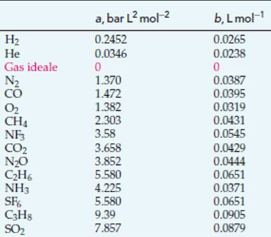
\includegraphics[width=0.5\linewidth]{../images/costantiaeb}
	\caption{Alcuni valori delle costanti a e b tabulati}
	\label{fig:costantiaeb}
\end{figure}
\FloatBarrier
Possiamo renderla più leggibile sostituendo il volume molare (indicato con $v$ minuscola), in questo modo l'equazione studia una sola mole di gas.  
\begin{align*} 
\left( p + \frac{a}{v^2}\right)\left(v-b\right) = R \theta
\end{align*} 

Proviamo ora a disegnare la funzione p(v) per la $CO_2$ sul piano di Clapeyron
\begin{figure}[h!]
	\centering
	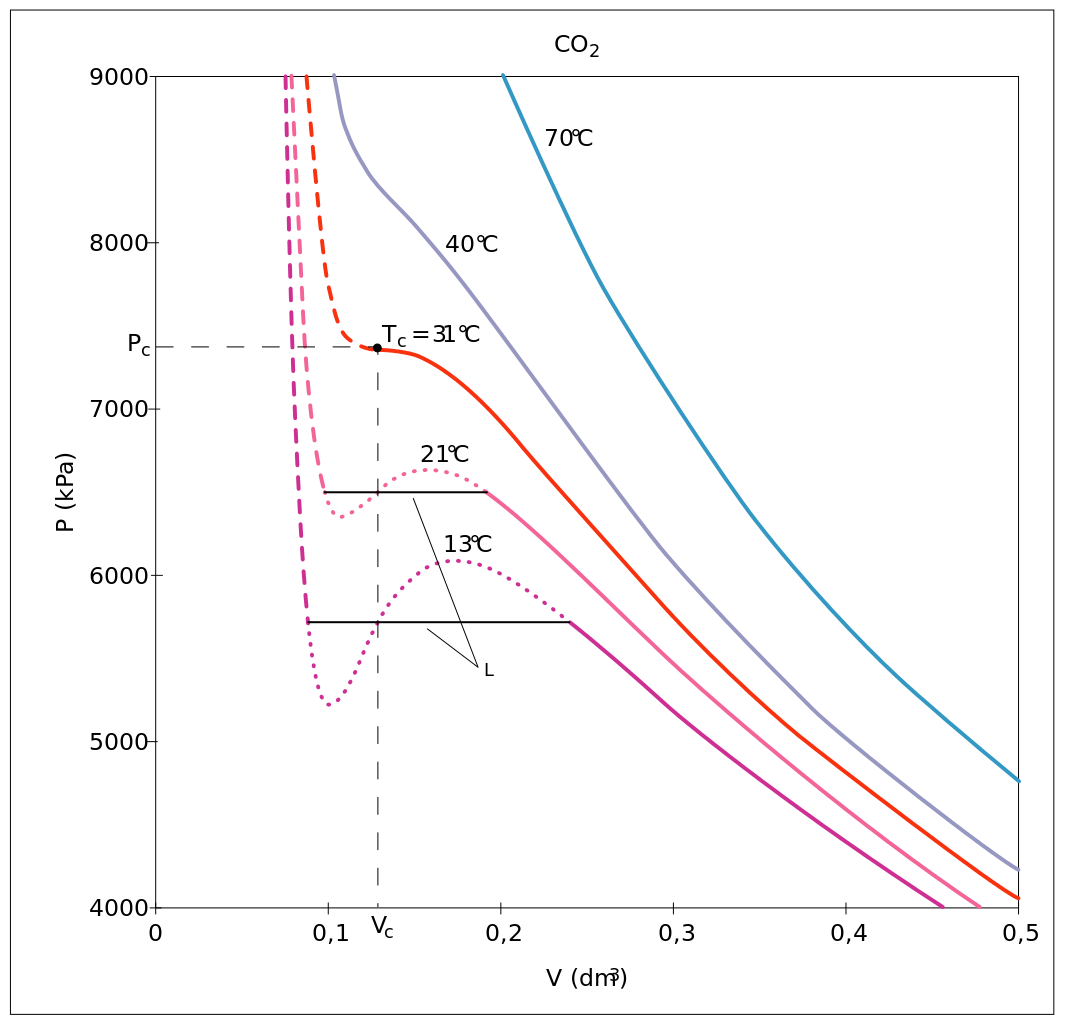
\includegraphics[width=0.6\linewidth]{../images/Van_der_Waals}
	\caption{Rappresentazione di curve di stato per la $CO_2$ a diverse temperature.}
	\label{fig:vanderwaals}
\end{figure}
\FloatBarrier
Ogni curva corrisponde ad un valore di temperatura. Come vediamo, per alte temperature si ha una figura che approssima un ramo d'iperbole, proprio come per i gas perfetti, ciò perché le molecole hanno più energia cinetica e risentono meno delle interazioni intermolecolari. Diminuendo la temperatura osserviamo che la curva comincia a piegarsi fino ad arrivare ad una temperatura critica in cui si genera un flesso. Con considerazioni matematiche è possibile calcolare le coordinate (pressione e volume molare critici) del flesso a temperatura critica $\theta_c$. Innanzi tutto poniamo derivata prima e seconda uguali a zero per poi dividere membro a membro, ricavare il volume molare critico, sostituirlo in una delle due equazioni e ricavare $\theta_c$ (si presuppone che a e b siano noti). 
\begin{align*} 
&\begin{cases}
	\frac{\partial p}{\partial v} = -\frac{R \theta_c}{(v_c - b)^2} + \frac{2a}{v_c^3} = 0\\
	\frac{\partial^2 p}{\partial v^2} = \frac{2 R \theta_c}{(v_c - b)^3} - \frac{6 a}{v_c^4} = 0
\end{cases}\\\\
&\begin{cases}
	\frac{R \theta_c}{(v_c - b)^2} = \frac{2a}{v_c^3}\\
	\frac{2 R \theta_c}{(v_c - b)^3} = \frac{6 a}{v_c^4} 
\end{cases}\\
&\frac{2}{(v_c-b)} = \frac{3}{v_c}\\ 
& \Rightarrow v_c = 3b\\
& \Rightarrow \theta_c = \frac{8a}{27 R b}\\
\end{align*} 
Una volta trovati $\theta_c$ e $v_c$ sostituiamo nell'equazione dei gas reali per ottenere $p_c$
\begin{align*} 
	p_c &= \frac{R \theta_c}{v_c - b}-  \left(\frac{a}{v_c^2}\right) = \\
	&\frac{R \frac{8a}{27 R b}}{3b - b}-  \left(\frac{a}{9b^2}\right) = \frac{a}{27 b^2}\\
\end{align*} 
Se invece a e b non fossero conosciuti, è possibile misurarli con le seguenti relazioni, derivanti dl precedente sistema. 
\begin{align*} 
\begin{cases}
a = \frac{9}{8} R \theta_c v_c\\
b = \frac{v_c}{3}
\end{cases}
\end{align*} 
\'{E} inoltre interessante calcolare il valore della costante di compressione alla temperatura critica ($z_c$) sostituendo i valori di volume pressione e temperatura critici ottenuti. 
\begin{align*} 
z_c = \frac{p_c v_c }{R \theta_c} = \frac{3}{8}
\end{align*} 
Ne deduciamo che il coefficiente di compressione di qualsiasi gas reale al punto critico è costante ed è pari a $\frac{3}{8}$. Questa è un'occasione per valutare se la teoria sviluppata si adatti bene all'esperienza, effettivamente i gas reali alla temperatura critica presentano con buona approssimazione di questo coefficiente di compressione.\\
Tornando al grafico (\ref{fig:vanderwaals}), le curve al di sotto della temperatura critica presentano una regione all'interno della quale il modello teorico non rispecchia la realtà; sperimentalmente si nota infatti un andamento costante, perché? Ciò è dovuto al cambiamento di stato (detto anche transizione di fase) del gas che comincia a condensare, producendo goccioline d'acqua. In questa regione il materiale si trova allo stato di \textbf{vapore saturo}: se si diminuisce il volume diminuiscono le molecole di gas e aumentano quelle di liquido. Ad un certo punto, quando il vapore sarà diventato completamente liquido, al diminuire del volume si avrà un aumento di pressione enorme, che conferisce l'alta pendenza delle curve nel lato sinistro. Ciò avviene perché un liquido è praticamente incomprimibile (servono pressioni enormi). Esiste inoltre un'altra regione in cui il gas è allo stato di \textbf{vapore} (si veda \ref{fig:diagramma-di-fase}). 
\begin{figure}[h!]
	\centering
	\includegraphics[width=0.6\linewidth]{../images/"diagramma di fase"}
	\caption{Diagramma di fase dell'acqua in cui sono distinte, con colori diversi, le regioni in cui si ha una specifica fase.}
	\label{fig:diagramma-di-fase}
\end{figure}
\FloatBarrier
Data una curva di van der Waals, è possibile trovare il segmento in cui la pressione è costante (transizione di fase vapore-liquido) seguendo la \textbf{costruzione di Maxwell}. Basterà scegliere il segmento che rende uguali le aree contenute fra la curva sovrastante il segmento ed il segmento stesso e fra il segmento e la curva sottostante il segmento. Si veda la figura per chiarimenti.
\begin{figure}
	\centering
	\includegraphics[width=0.5\linewidth]{../images/"calcolo di maxwell"}
	\caption{Il segmento compreso fra le intersezioni retta-curva rappresenta la transizione di fase, per ricavarlo bisogna che le due aree siano uguali.}
	\label{fig:calcolo-di-maxwell}
\end{figure}
\FloatBarrier
Il volume nell'estremità destra del segmento è il volume occupato dal gas quando è saturo ($V_g$), cioè quando una variazione infinitesima di volume fa cominciare la condensazione mentre il volume alla sinistra del segmento è quello occupato dal liquido ottenuto a seguito della transizione di fase ($V_l$). Tutti i valori di $V_g$ e $V_l$ al variare della temperatura formano una parabola rovesciata, con vertice nel punto di temperatura critica, che corrisponde con la regione a pressione costante a cui si accennava sopra. \\
Possiamo disegnare un grafico 3D in cui nel terzo asse poniamo la temperatura (fino ad ora abbiamo disegnato su uno stesso grafico 2D diverse sezioni del grafico 3D al variare di $\theta$) per distinguere 5 regioni: gas, vapore, vapore-liquido, liquido, solido più una sesta, non indicata nel grafico 3D ma presente in \ref{fig:diagrammadifasept} detta \textbf{regione supercritica} in cui si ha una condizione intermedia fra liquido e gas.  
\begin{figure}[h!]
	\centering
	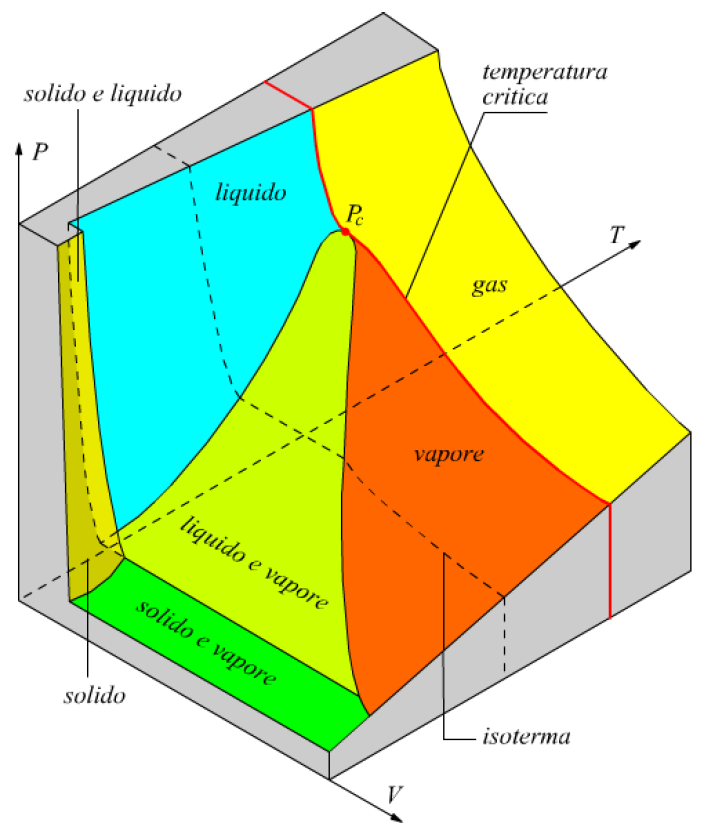
\includegraphics[width=0.5\linewidth]{../images/diagrammadifase3D}
	\caption{Versione 3D del diagramma di fase.}
	\label{fig:diagrammadifase3d}
\end{figure}
\FloatBarrier
Possiamo notare inoltre che sotto una determinata temperatura avviene la transizione allo stato solido e che possiamo individuare un segmento in cui si ha uno stato intermedio fra quello di solido vapore e liquido, quelli sono i punti tripli al variare della temperatura. \'{E} interessante citare la regola delle fasi di Gibbs che ora risulta chiara: dette N il numero di gradi di libertà, F il numero di fasi e C il numero di componenti indipendenti che formano il composto, la legge di Gibbs afferma
\begin{align*} 
	N = C + 2 - F
\end{align*}  
Ciò si applica perfettamente alla temperatura critica, infatti in questo caso C = 1, F = 3 e allora avremo zero gradi di libertà, cioè un punto. Per il punto critico invece avremo 1 grado di libertà e quindi una retta (con parametro V) e così via.\\
Inoltre, possiamo guardare la proiezione del grafico 3D sul piano PT per ottenere diverse informazioni. 
\begin{figure}[h!]
	\centering
	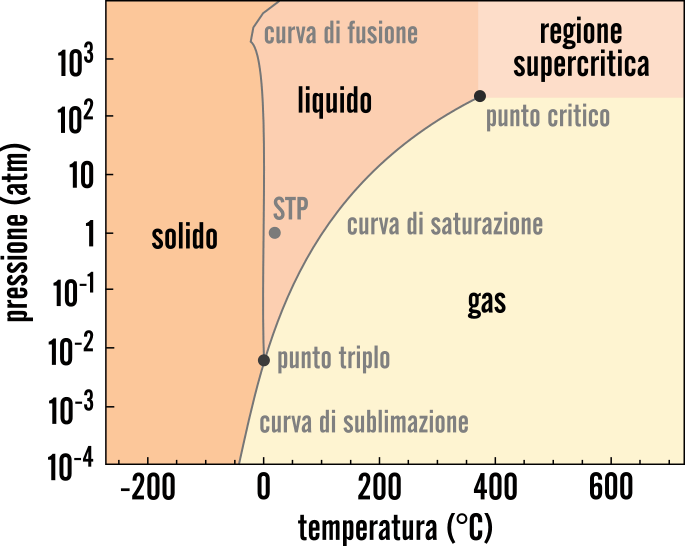
\includegraphics[width=0.6\linewidth]{../images/diagrammadifasePT}
	\caption{Diagramma di fase sul piano PT}
	\label{fig:diagrammadifasept}
\end{figure}
\FloatBarrier
Le curve (una per la solidificazione, una per la liquefazione e una per la sublimazione) sono l'insieme delle temperature di passaggio di stato possibili al variare della pressione. Ad esempio, vediamo come la temperatura di ebollizione aumenti all'aumentare della pressione. Inoltre possiamo apprezzare il punto triplo: l'intersezione delle tre curve. Il processo di cambiare stato da liquido a gassoso a temperatura costante variando la pressione si chiama cavitazione. Per temperature superiori a quella critica lo stato è detto \textbf{supercritico}, con caratteristiche intermedie fra quelle di liquido e di gas. 
\section{Teoria cinetica dei gas} \label{sec:teoriacinetica}
Vogliamo ora interpretare alcune grandezze fisiche macroscopiche introdotte precedentemente, (in particolare pressione e temperatura) dal punto di vista microscopico. Per far ciò, a partire dalla teoria della meccanica classica costruiremo il modello di una scatola piena di gas perfetto e la analizzeremo dal punto di vista microscopico. Se il modello e la teoria sono corretti, allora dovremo avere un riscontro empirico nella realtà, altrimenti dovremo modificare il modello (problema relativamente risolvibile) o, più drammaticamente, dovremo modificare la teoria. Cominciamo con il definire le caratteristiche del nostro modello. 
\begin{enumerate}
	\item Numero N di molecole nel cubo molto grande 
	\item Covolume trascurabile (molecole puntiformi)
	\item Interazioni intermolecolari a lungo raggio trascurabili e interazioni a corto raggio (urti tra molecole o tra molecola e parete) totalmente elastiche 
	\item Caos molecolare (ovvero isotropia e omogeneità delle molecole nel volume)
\end{enumerate} 
Vediamo ora se un $cm^3$ di aria rispetta queste condizioni:\\
1) Calcoliamo il numero di molecole di aria in un $cm^3$. 
\begin{align*} 
	&pV =nR\theta = \frac{N}{N_a} R\theta\\
	&N = \frac{pV N_a}{R\theta} = \frac{1.013\ 10^5\ 10^{-6}\ 6 10^{23}}{8.314\ 300} = 2.5 10^{19}\ \text{molecole}
\end{align*} 
Che è sufficientemente grande, anche su scale locali, per consentire un approccio statistico al problema, infatti l'incertezza sulla media sarebbe, considerando che questo sia un esperimento di conteggio, $\frac{1}{\sqrt{N}}$ .\\\\
2) Assumendo per le molecole di $O_2$ ed $N_2$ (i maggiori costituenti dell'aria) un diametro di 1.7 ${\AA}$, stimiamo la frazione di volume libero di cui dispone ogni molecola del punto 1
\begin{align*} 
	&d = 1.7 \AA\\
	&V_{1mol} = N \frac{4}{3}\pi \frac{d}{2}^3 \simeq N \frac{d^3}{2} \simeq 6 10^{-11}\ m^3\\
	&r = \frac{V_{1mol}}{V_c} = \frac{6 10^{-11}}{10^{-6}} = 6 10^{-5}\ m^3\\
\end{align*} 
Dove $V_c$ è il volume della scatola di lato l che contiene il gas ed r è un coefficiente che indica il rapporto fra il covolume di una mole di gas (ovvero la summa dei volumi occupati dalle sue particelle) ed il volume del contenitore, che consideriamo abbastanza bassa. \\\\
3)Possiamo stimare la distanza media tra le molecole dividendo il volume del contenitore per il numero di molecole, così da sapere il volume che ha a disposizione ogni molecola. Se immaginiamo questo volume cubico possiamo poi farne a radice cubica per ottenere la distanza media fra molecole.
\begin{align*} 
	\lambda = \sqrt[3]{\frac{V_c}{N}} = \sqrt[3]{\frac{10^{-6}}{2.5 10^{13}}}= 3.4 10^{-3}\ m \simeq 34\AA
\end{align*} 
Questa distanza è circa 20 volte il diametro della molecola meda d'aria (citato nel punto 2). Visto che il valore $r_{min}$ (ovvero la distanza a cui potenziale attrattivo e repulsivo si eguagliano) è comparabile a quello del diametro della molecola, anch'esso sarà 20 volte minore al valore calcolato di $\lambda$, ciò vuol dire che le molecole ad una distanza $\lambda$ sono in una regione sufficientemente a destra del grafico di Lennard-Jones per stimare le interazioni a lungo raggio trascurabili. Infine, gli urti con le pareti sono chiaramente elastici poiché le molecole d'aria sono tanto piccole da poter essere approssimate a puntiformi, cioè senza gradi di libertà interni mentre gli urti fra molecole, essendo la scatola prevalentemente vuota (a causa del rapporto r molto basso) non avverranno praticamente urti fra molecole.\\\\
4) Omogeneità significa che la densità è costante in tutto il recipiente (cioè non ci sono addensamenti o rarefazioni) mentre isotropia vuol dire che non ci sono direzioni privilegiate, ovvero che per ogni molecola che si muove in un verso ne esiste un'altra che si muove in verso opposto. Ciò si traduce in una velocità media nulla ovvero $\sum_i \vec{v}_i = 0$. Il gas è macroscopicamente fermo.\\\\
Possiamo ora calcolare la pressione che genera il gas sulla parete, concentriamoci sulla parete $S_x$ di destra, perpendicolare all'asse x. Calcoliamo la pressione come l'impulso complessivo scambiato in un certo intervallo di tempo dall'insieme delle molecole con la parete. Considerando inizialmente una qualsiasi particella i-esima di velocità $\vec{v}_i$ che si muove obliquamente e collide con la parete destra, si avrà che la componente della velocità in x cambierà di segno mentre le altre componenti rimarranno invariate.
\begin{align*} 
	\begin{cases}
		v'_{ix}=v_{ix} \Rightarrow \Delta q_{ix} = mv'_{ix}-(-mv'_{ix})=-2mv_{ix}\\
		v'_{iy}=v_{iy} \Rightarrow \Delta q_{iy} = 0\\
		v'_{iz}=v_{iz} \Rightarrow \Delta q_{iz} = 0
	\end{cases}
\end{align*} 
In un intervallo di tempo $\Delta t$ la particella i-esima colpisce la parete destra un numero di volte unicamente proporzionale alla componente x di $\vec{v}_i$ per l'intervallo di tempo (ovvero lo spazio percorso in quel tempo) e inversamente proporzionale alla distanza che deve compiere, che sarà $2l$ ovvero due volte il lato del cubo. 
\begin{align*} 
	&n_u = \frac{|v_{ix}| \Delta t}{2l}\\
	&|\Delta Q_{ix}|= |\Delta q_{ix}| n_u = (2m|v_{ix}|) \frac{|v_{ix}| \Delta t}{2l} = m v_{ix}^2 \frac{\Delta t}{l}\\
	&|\Delta Q_{x}| = \sum_i |\Delta Q_{ix}|= \frac{m \Delta t}{l} \sum_i v_{ix}^2 
\end{align*} 
Dove nella penultima riga abbiamo moltiplicato l'impulso generato da un urto per il numero d'urti in un intervallo di tempo $\Delta t$ mentre nell'ultima abbiamo tenuto conto di tutte le particelle sommando gli i impulsi. Quest'ultima forma rappresenta l'impulso esercitato dalle collisioni di una molecola con la parete in un intervallo di tempo $\Delta t$.
Possiamo ora volutare la forza e la pressione esercitati dalla molecola in un intervallo di tempo. 
\begin{align*} 
	&F_x = \frac{|\Delta Q_{x}|}{\Delta t} =  \frac{m}{l} \sum_i v_{ix}^2\\
	&p_x = \frac{F_{x}}{S_x} =  \frac{1}{l^2}\frac{m}{l} \sum_i v_{ix}^2=\frac{m}{l^3} \sum_i v_{ix}^2 = \frac{m}{V_c} \sum_i v_{ix}^2
\end{align*} 
Possiamo ripetere considerazioni analoghe per ottenere l'espressione della pressione sulle altre pareti
\begin{align*} 
	\begin{cases}
		p_x = \frac{m}{V_c} \sum_i v_{ix}^2\\
		p_y = \frac{m}{V_c} \sum_i v_{iy}^2\\
		p_z = \frac{m}{V_c} \sum_i v_{iz}^2
	\end{cases}
\end{align*} 
Per l'ipotesi del caos molecolare, non esiste una direzione privilegiata verso cui si muovono le molecole per cui le velocità nei diversi assi sono statisticamente uguali. Per l'ipotesi di un N molto grande le fluttuazioni statistiche sono molto ridotte per cui possiamo approssimare, entro gli errori di misura, che 
\begin{align*} 
	p_x = p_y = p_z \equiv p
\end{align*} 
Abbiamo così ricavato il \textbf{principio di Pascal}, che afferma, in forma semplice, che la pressione esercitata da un fluido su un contenitore è uguale in ogni punto della superficie.\\
Possiamo dunque scrivere
\begin{align*} 
	&p_x+p_y+p_z = 3p = \frac{m}{V} \sum_i (v_{ix}^2+v_{iy}^2+v_{iz}^2) = \frac{m}{V} \sum_i v_i^2\\
	&pV = \frac{m}{3}\sum_i v_i^2
\end{align*} 
Possiamo introdurre la velocità quadratica media, per poi sostituirla nella formula ed effettuare alcuni passaggi
\begin{align*} 
	&\overline{v^2} \equiv \sum_i\frac{v_i^2}{N}\\
	&pV = \frac{m}{3}N \overline{v^2} = \frac{2}{3} N (\frac{1}{2}m \overline{v^2})=\frac{2}{3}N \overline{\varepsilon}\\
\end{align*} 
Dove $\overline{\varepsilon}$ è detta energia cinetica media ed è definita come
\begin{align*} 
	\overline{\varepsilon} \equiv \frac{1}{2} m \overline{v^2} = \frac{1}{2} m \sum_i\frac{v_i^2}{N}
\end{align*} 
La connessione per passare dall'approccio microscopico a quello macroscopico ci è offerta dall'equazione di stato dei gas perfetti
\begin{align}\label{eq:energiacinmedia}
	&pV = n R \theta = \frac{2}{3}N \overline{\varepsilon}\nonumber\\
	\Rightarrow & \overline{\varepsilon} = \frac{3}{2} \frac{R}{N_a} \theta = \frac{3}{2}k_b\theta
\end{align} 
dove nell'ultimo passaggio è stata sostituita la costante k, detta \textbf{costante di Boltzmann}, definita come
\begin{align*} 
k_b = \frac{R}{N_a}
\end{align*} 
misurabile mediante esperimenti, come quello di Perrin sul moto browniano.\\ 
La (\ref{eq:energiacinmedia}) collega la temperatura (grandezza macroscopica) all'energia cinetica media (grandezza microscopica), ciò ci suggerisce che misurare la temperatura è perfettamente equivalente a misurare l'energia cinetica media in una diversa unità di misura, che differisce dai kelvin semplicemente per una costante. Ora è possibile introdurre il concetto di \textbf{zero assoluto} ovvero, il limite inferiore di temperatura possibile (solamente approssimabile) in cui tutte le molecole del gas sono in quiete, cioè quando hanno energia cinetica nulla.

\subsection{Energia cinetica e gradi di libertà}\label{sec:energiacinetica_d.o.f.}
\'{E} utile notare che il 3 al denominatore nella (\ref{eq:energiacinmedia}) proviene dai 3 gradi di libertà della molecola di gas, che è ipotizzato perfetto e dunque come formato da particelle puntiformi con 3 d.o.f.(che da ora chiameremo $\nu$). Intuitivamente, ripercorrendo i passi fatti, a causa del caos molecolare siamo portati ad aggiungere uno stesso termine \((\frac{1}{2}k\theta)\) per ogni grado di libertà. 
\begin{align*} 
	\overline{\varepsilon} = \frac{1}{2}m\overline{ v^2} = \frac{1}{2}m\overline{ v_x^2}+\frac{1}{2}m\overline{ v_y^2}+\frac{1}{2}m\overline{ v_z^2} = \frac{1}{2}k\theta+\frac{1}{2}k\theta+\frac{1}{2}k\theta
\end{align*}  
Esiste un teorema che generalizza e formalizza questa intuizione (per ora si fornisce solo l'enunciato, che verrà dimostrato in seguito).
\begin{theorem}[Equipartizione delle energie]
	Ad ogni grado di libertà $\nu$ che compare quadraticamente nell'espressione dell'energia si associa il valore \(\frac{1}{2}k\theta\)
\end{theorem}
Possiamo così riscrivere la formula dell'energia
\begin{align}\label{eq:energiacinetica_d.o.f.}
	&\overline{\varepsilon} = \frac{\nu}{2} k \theta\\
	&\theta = \frac{2 \overline{\varepsilon}}{k \nu}\nonumber
\end{align} 
Si approfondisce il significato fisico di questo risultato nella sezione (\ref{sec:energia_interna_mono_bi_poli})
\subsection{$k_b$ come costante esatta}
Dal novembre 2018 si è decisa una nuova strategia di misurazione del grado Kelvin: si è definita la $k_b$ come costante con il valore esatto
\begin{align*} 
	k_b \equiv 1.380649 \cdot 10^{-23}
\end{align*} 
priva di errore, si è dunque definita la temperatura di 1 Kelvin come la temperatura che possiede un corpo la cui energia cinetica media per ogni grado di libertà è $\frac{k_b}{2}$. Inoltre, dalla definizione della costante di Boltzmann, ricaviamo che l'aumento di un Kelvin di temperatura di una sostanza corrisponde ad un aumento di energia cinetica media di $k_b$ Kelvin. 
\begin{align*} 
	1\ K = k_b\ J
\end{align*}  
Ecco il fattore di conversione da Kelvin a Joule.\\
Nella fisica nucleare non è comodo usare i Joule, unità di misura utile nel mondo macroscopico, per questo si fa uso degli \textbf{elettronvolt}, definito come l'energia di un elettrone accelerato da un Volt. Da ciò si ha 
\begin{align*} 
	1\ eV = q\ J
\end{align*} 
Dove q è la carica dell'elettrone. Da ciò possiamo ricavare la relazione fra $eV$ e $J$.
\begin{align*} 
	1\ eV = \frac{q}{k_b}\ K = J = \frac{1.6\cdot 10^{-19}}{1.38\cdot10^{-23}}=\simeq 1.6 \cdot 10^4
\end{align*} 

\subsection{Deduzione della p.d.f. delle velocità}
Abbiamo dedotto il valore dell'energia cinetica media, calcolata mediante la velocità quadratica media. Vogliamo ora sapere quale sia la distribuzione delle velocità da cui si estrae la velocità quadratica media. Vogliamo trovare la p.d.f. di
\begin{align*} 
	v \equiv |\vec{v}| = \sqrt{v_x^2+v_y^2+v_z^2}
\end{align*} 
Cominciamo con il ricavare la \textbf{p.d.f. congiunta} $f(v_x, v_y, v_z)$, ovvero la probabilità di avere contemporaneamente le velocità sui tre assi in un intorno di ampiezza infinitesima. Per capire meglio cominciamo consideriamo il caso con una velocità unidimensionale, la p.d.f. è $f(v_x)$, per calcolare la probabilità che $v_x$ stia in un intorno basterà integrare fra gli estremi di quell'intorno
\begin{align*} 
	& P(v'_x<v_x<v'_x+dx)= \int_{v_x}^{v_x+dx}f(v_x)dx
\end{align*} 
Estendendo il concetto ai 3 assi si parla di p.d.f. congiunta (in questo caso congiunta è sinonimo di trivariata) che sarà $f(v_x, v_y, v_z)$, per trovare la probabilità ora dobbiamo fare un integrale triplo
\begin{align*} 
	&P(v'_x<v_x<v'_x+dx, v'_y<v_y<v'_y+dy, v'_z<v_z<v'_z+dz) =\\
	&\int_{v_x}^{v_x+dx}\int_{v_y}^{v_y+dy}\int_{v_z}^{v_z+dz} f(v_x,v_y,v_z) dxdydz
\end{align*} 
Possiamo vedere la probabilità P geometricamente su un grafico f(v) su v 3D come la probabilità che la velocità sia contenuta in un parallelepipedo di lati $dx, dy, dz$.\\
Essendo la velocità su ogni asse indipendente dalle altre la probabilità di trovare in un intorno specifico ogni componente della velocità sarà semplicemente il prodotto delle probabilità delle singole componenti.
\begin{align}\label{eq:cond1}
	&f(v_x, v_y, v_z) = f(v_x)\cdot f(v_y)\cdot f(v_z)\\
	& P(v'_x<v_x<v'_x+dx, v'_y<v_y<v'_y+dy, v'_z<v_z<v'_z+dz) =\nonumber\\ 
	&P(v'_x<v_x<v'_x+dx) P(v'_y<v_y<v'_y+dy) P(v'_z<v_z<v'_z+dz)=\nonumber\\
	&\int_{v_x}^{v_x+dx} f(v_x)dx \cdot \int_{v_y}^{v_y+dy}f(v_y)dy \cdot \int_{v_z}^{v_z+dz}f(v_z)dz\nonumber
\end{align} 
A noi interessa la distribuzione del modulo delle velocità delle molecole dunque la p.d.f. congiunta che cerchiamo deve dipendere da $(v_x^2+v_y^2+v_z^2)$ ovvero il modulo della velocità (non ci interessa la radice ma semplicemente che dipenda dalla somma quadratica, in modo da annullare il contributo del segno). Ne segue che la p.d.f. deve rispettare la condizione
\begin{align}\label{eq:cond2}
	f(v_x,v_y,v_z) = f(v_x^2+v_y^2+v_z^2)
\end{align} 
Come intuì lo stesso Maxwell, l'unica funzione che rispetta contemporaneamente le condizioni (\ref{eq:cond1}) e (\ref{eq:cond2}) è quella esponenziale, infatti
\begin{align*} 
	e^{a^2+b^2+c^2}=e^{a^2} e^{b^2} e^{c^2}
\end{align*} 
Dunque possiamo ipotizzare che la p.d.f. della velocità su un singolo asse è
\begin{align*} 
	f(v_i) = \eta e^{\pm \xi v_i^2}
\end{align*} 
Possiamo escludere il "+" sin da subito sia per considerazioni matematiche, infatti l'integrale della funzione da $- \infty$ a $+ \infty$ deve fare 1 e se non fosse un esponente negativo l'integrale andrebbe ad infinito; ma anche per considerazioni fisiche, infatti se la densità di probabilità fosse sempre crescente allora sarebbe sempre molto più probabile trovare molecole molto veloci rispetto a molto lente, ciò è chiaramente assurdo perché ci aspettiamo un valore di velocità medio e nelle code della distribuzione valori molto alti e molto bassi egualmente poco probabili.\\
Con il segno meno abbiamo dunque una p.d.f. del tipo di una gaussiana. Ricaviamo dunque le costanti $\eta$ e $\xi$. la prima la ricaviamo sfruttando la condizione di normalizzazione ad 1 delle p.d.f.
\begin{align*} 
	\int_{-\infty}^{+\infty} f(v_i)dv_i = \eta \int_{-\infty}^{+\infty} e^{\pm \xi v_i^2} dv_i = 1
\end{align*} 
Questo è detto \textbf{integrale di Laplace} la cui risoluzione è in Appendice. Ne risulta che
\begin{align*} 
	\eta = \sqrt{\frac{\xi}{\pi}}
\end{align*} 
Per ricavare $\xi$ calcoliamo la velocità quadratica media ricordando la definizione di momento del secondo ordine di una p.d.f.
\begin{align*} 
	&\overline{v^2} \equiv \int_{-\infty}^{+\infty} v_i^2 f(v_i)dv_i = \frac{1}{2\xi}\\
	&\overline{v^2} = \overline{v_x^2}+\overline{v_y^2}+\overline{v_z^2} = 3\overline{ v_i^2} = \frac{3}{2\xi}
\end{align*} 
Ricordando ora la relazione che lega velocità quadratica media e temperatura (\ref{eq:energiacinmedia}) sostituiamo
\begin{align*} 
	&\frac{3}{2} k_b \theta = \overline{\varepsilon} = \frac{1}{2} m \overline{v^2}\\
	\Rightarrow & \overline{v^2} = \frac{3k_b\theta}{m}\\
	&\xi = \frac{m}{2k_b\theta} \quad \eta = \sqrt{\frac{m}{2\pi k_b \theta}}
\end{align*} 
Possiamo dunque riscrivere la p.d.f.
\begin{align*} 
	f(v_i) = \sqrt{\frac{m}{2\pi k_b\theta}} e^{-\frac{m v_i^2}{2 k_b \theta}}
\end{align*} 
\begin{figure}[h!]
	\centering
	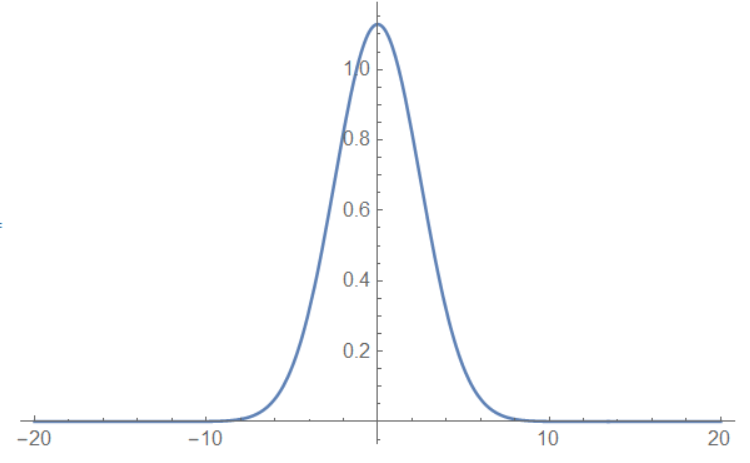
\includegraphics[width=0.6\linewidth]{../images/gausspdf}
	\caption{Funzione di distribuzione di probabilità (p.d.f.) della velocità lungo l'asse x (gaussiana).}
	\label{fig:gausspdf}
\end{figure}
\FloatBarrier

Osservando questa p.d.f. gaussiana possiamo trarne alcune caratteristiche fondamentali: 
\begin{align*} 
	\mu = 0 \quad \sigma = \sqrt{\frac{k_b \theta}{m}}
\end{align*} 
Il fatto che la curva abbia media in zero non ci stupisce poiché, essendo in ipotesi di caos molecolare le velocità di segno diverso si cancellano statisticamente. Inoltre notiamo che la varianza, ovvero la larghezza della curva, è direttamente proporzionale alla temperatura, ciò avviene perché l'aumento di temperatura equivale ad un aumento delle velocità, che continueranno ad annullarsi reciprocamente ma che non saranno singolarmente nulle.\\
Essendo le p.d.f. indipendenti, per ottenere la p.d.f. congiunta basta moltiplicarle
\begin{align*} 
	f(v_x, v_y,v_z) = \left(\frac{m}{2\pi k_b\theta}\right)^{\frac{3}{2}} e^{-\frac{m( v_x^2+v_y^2+v_z^2)}{2 k_b \theta}} = \left(\frac{m}{2\pi k_b\theta}\right)^{\frac{3}{2}} e^{-\frac{m v^2}{2 k_b \theta}}
\end{align*} 
A partire dalla congiunta possiamo ricavare la p.d.f. del modulo del vettore velocità. Se la $f(v_x, v_y,v_z)$ era rappresentabile geometricamente come un cubo all'interno del quale si trovava la probabilità di trovare una molecola nell'intorno di un'esatta terna di valori (ad esempio $(v_x \in I_{dx}(a), v_y \in I_{dy}(b), v_z = \in I_{dz}(c)))$ . Noi vogliamo invece trovare una p.d.f. che ci dica la probabilità che il modulo del vettore velocità si trovi in un certo intorno cioè $ \sqrt{v_x+v_y+v_z} \in I_{dv}(v)$. Risulta chiaro che esistono diverse terne di intorni che soddisfano quest'ultima relazione. In particolare l'insieme di queste terne è il luogo geometrico dei punti a distanza dal centro compresa fra v e dv. Chiaramente otterremo un guscio sferico di spessore dv. Per calcolare la p.d.f. ($\rho(v)$) moltiplichiamo il volume del guscio per la probabilità associata all'unità di volume (ovvero quella del cubetto $f(v_x,v_y, v_z)$)
\begin{figure}[h!]
	\centering
	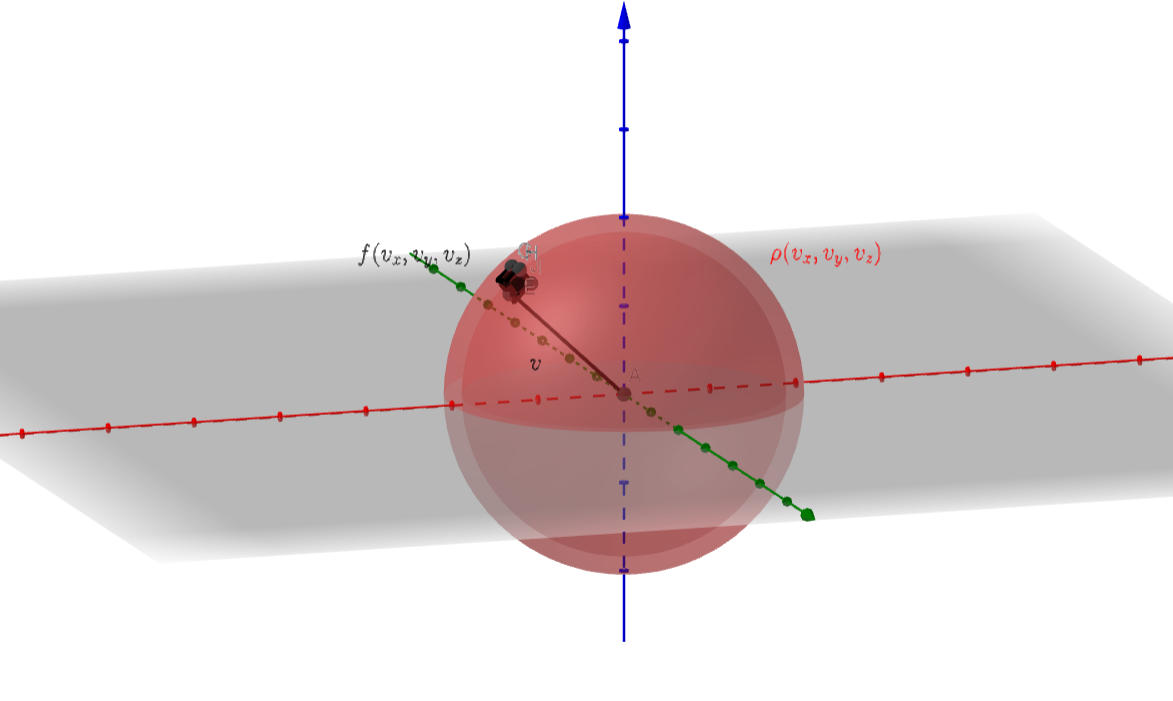
\includegraphics[width=0.7\linewidth]{../images/guscio}
	\caption{Grafico qualitativo della p.d.f. $\rho(v_x,v_y,v_z)$ a confronto con quella di $f(v_x, v_y, v_z)$}
	\label{fig:guscio}
\end{figure}
\FloatBarrier
\begin{align}\label{eq:pdfMaxwellvelocità}
	&\rho(v) dv = f(v_x, v_y, v_z) 4\pi v^2 dv \nonumber \\
	&\rho(v)=\frac{4}{\sqrt{\pi}}\left(\frac{m}{2k_b\theta}\right)^{\frac{3}{2}} v^2 e^{-\frac{mv^2}{2 k_b \theta}}
\end{align} 
Questa è detta di \textbf{p.d.f. di Maxwell-Boltzmann}. Offre una quantità di informazioni molto interessanti: possiamo calcolare il modulo velocità media ad ogni temperatura, conoscere il numero di molecole atteso che abbia una velocità compresa in un certo intervallo... \'{E} interessante che con questo grafico possiamo spiegare un semplice evento della vita quotidiana: perché i panni si asciugano una volta stesi? In teoria per far evaporare l'acqua bisognerebbe riscaldare l'acqua ad un punto tale che l'energia cinetica delle singole molecole è tale da rompere i legami intermolecolari e "scappare", se però non facciamo riscaldare i panni fino a 100 \textdegree C (temperatura di ebollizione dell'acqua) come fanno a scappare queste molecole? la risposta è che non tutte le molecole hanno la stessa velocità e che questa è distribuita in base ad una p.d.f.: esiste una soglia dopo la quale la velocità delle molecole è tale da poter rompere il legame, ed esiste una probabilità che si trovino molecole a questa velocità anche se in media le molecole hanno una velocità minore. Chiaramente, maggiore la temperatura maggiore sarà la probabilità di trovare molecole oltre questa soglia. Ecco perché al caldo i panni si asciugano più velocemente!
\begin{figure}[h!]
	\centering
	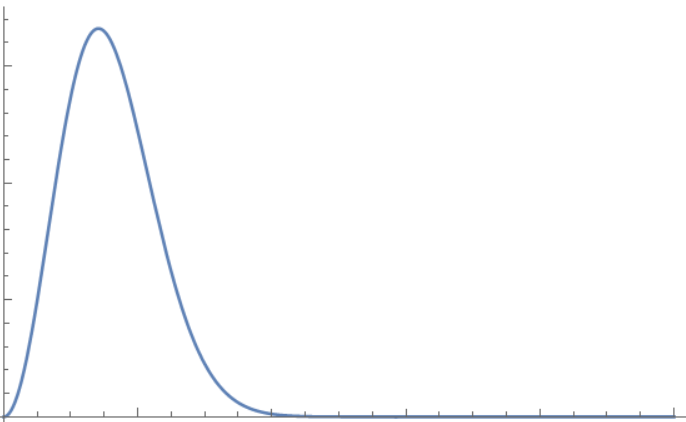
\includegraphics[width=0.6\linewidth]{../images/speedpdf}
	\caption{Funzione di distribudione delle probabilità (p.d.f.) del modulo della velocità detta di Maxwell-Boltzmann}
	\label{fig:speedpdf}
\end{figure}
 \FloatBarrier
A partire da questa distribuzione possiamo ricavare alcuni parametri interessanti:
\begin{itemize}
	\item Valore più probabile o moda
	\begin{align*} 
		&\rho'(v)  =  0\\
		&v_p = \sqrt{\frac{2R\theta}{M}}
	\end{align*} 
	\item Valore atteso o di aspettazione (applicando la definizione per distribuzioni continue)
	\begin{align*} 
		\overline{v} = \int_{-\infty}^{\infty}v \rho(v)dv = \sqrt{\frac{8R\theta}{\pi M}}
	\end{align*} 
	\item valore quadratico medio (applicando la definizione per distribuzioni continue)
	\begin{align*} 
			\sqrt{\overline{v^2}} = \left(\int_{-\infty}^{\infty}v^2 \rho(v)dv\right)^{\frac{1}{2}} = \sqrt{\frac{3k\theta}{m}}= \sqrt{\frac{3R\theta}{M}}
	\end{align*} 
\end{itemize}
Si noti che questi valori, nonostante simili, non sono uguali, ciò è dovuto all'asimmetria della distribuzione. 
\begin{align*} 
	v_p<\overline{v}<\sqrt{\overline{v^2}}
\end{align*} 
\begin{exercise}
	Calcolare i valori tipici delle velocità molecolari di $H_2$ e $N_2$ a temperatura ambiente (300 K).
	\begin{align*} 
		\sqrt{\overline{v^2}}_{H_2}=\sqrt{\frac{3\cdot 8.3145\cdot 300}{2\cdot 10^{-3}}}=1934\ \frac{m}{s}\\
			\sqrt{\overline{v^2}}_{N_2}=\sqrt{\frac{3\cdot 8.3145\cdot 300}{28\cdot 10^{-3}}}=493\ \frac{m}{s}\\
	\end{align*} 
\end{exercise}
Vogliamo ora verificare empiricamente che la distribuzione trovata rispecchi la realtà. esistono varie apparecchiature sperimentali, in questa sede ne descriveremo una delle più semplici e rudimentali: \textbf{il selettore di velocità}. Questo è formato da un contenitore cubico pieno di gas (il tutto a temperatura e pressione costanti) al quale su una faccia è applicato un foro da cui escono alcune molecole di gas con diverse velocità. Di fronte alla faccia forata è posizionato un selettore, ovvero uno schermo a cui è applicato un ulteriore foro, allineato con il primo, che permette il passaggio solamente delle molecole in direzione ortogonale alla faccia del contenitore. Le molecole selezionate viaggeranno su una retta ed avranno diverse velocità. Una volta superato il selettore le molecole incontrano un cilindro di raggio R con una fenditura verticale che ruota sul suo asse a velocità angolare $\omega$ fissata; nella superficie interna del cilindro è posizionata una pellicola che riesce a rilevare l'impatto (cambiando colorazione) di una molecola. Ora, a seconda della velocità delle molecole il tempo impiegato nel percorrere il diametro del cilindro (da quando entrano la fenditura a quando collidono con il cilindro) è inversamente proporzionale alla velocità, dunque se la teoria è corretta dovremmo vedere una regione con molte collisioni in corrispondenza della velocità più probabile e poi sempre minori collisioni allontanandosi, con una diminuzione proporzionale a quanto previsto dalla distribuzione.\\
La dipendenza della distanza dalla velocità è
\begin{align*} 
	&v = \frac{2R}{\Delta t} \Rightarrow \Delta t = \frac{2R}{v}\\
	&\Delta l = l-l_0 = \alpha R = \omega \Delta t=\omega \frac{2R}{v}R = \frac{2 \omega R^2}{v} 
\end{align*} 

Se immaginiamo, una volta finito l'esperimento, di srotolare il cilindro in un rettangolo, avremo che $l_0$ è il segmento passante per i punti medi delle basi del rettangolo ed $l$ la posizione di una generica rilevazione di impatto di una molecola (dunque $\Delta l$ sarà la distanza della rilevazione dal centro).  Questa distanza è uguale all'angolo in radianti spazzato nel tempo $\Delta t$ per il raggio (dalla definizione di radiante).
\begin{figure}[h!]
	\centering
	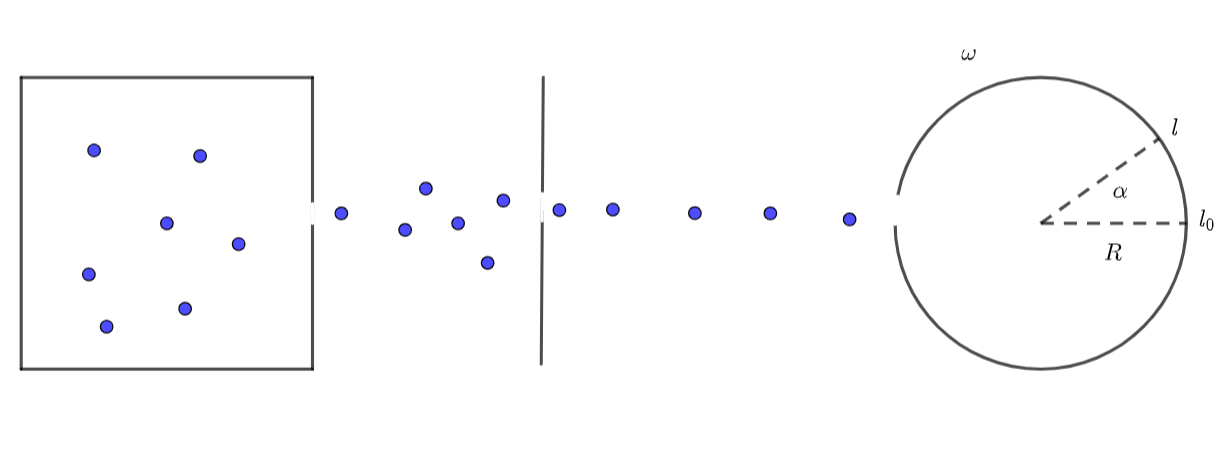
\includegraphics[width=0.9\linewidth]{../images/Esperimento_Maxwell}
	\caption{Diagramma dell'apparato sperimentale per la conferma empirica della distribuzione di Maxwell}
	\label{fig:esperimentomaxwell}
\end{figure}
\FloatBarrier
Per trovare le velocità delle singole molecole basterà misurare la distanza $\Delta l$ e inserirla nella formula
\begin{align*} 
	&v =\frac{2 R}{\Delta\tau}\\
	&\Delta l = \alpha R = \omega \Delta\tau R = \frac{\omega 2 R^2}{v}\\
	&\Rightarrow v = \frac{2\omega R^2}{\Delta l}
\end{align*} 
Dalla distribuzione delle molecole nel cilindro è possibile ricavare la distribuzione delle velocità che è compatibile con una distribuzione Maxwelliana entro gli errori.
\subsection{Ricavare la distribuzione delle energie da quella delle velocità}
Per passare dalla p.d.f. delle velocità a quella delle energie, ci avvaliamo dell'uguaglianza
\begin{align*} 
	\rho(\varepsilon)d\varepsilon = \rho(v)dv \Rightarrow \rho(\varepsilon) = \rho(v)\frac{dv}{d\varepsilon}
\end{align*} 
dove le $\rho(x)$ indicano le rispettive p.d.f.\\
Conoscendo la relazione
\begin{align*} 
	\varepsilon = \frac{1}{2}m v ^2 \Rightarrow v = \sqrt{\frac{2 \varepsilon}{m}}
\end{align*} 
Possiamo ricavare 
\begin{align*} 
	\frac{dv}{d\varepsilon} = \sqrt{\frac{1}{2 m \varepsilon}}
\end{align*} 
Da sostituire nell'espressione di $\rho(\varepsilon)$ insieme al noto $\rho(v)$ ricavato nella (\ref{eq:pdfMaxwellvelocità}).
\begin{align*} 
	\rho(\varepsilon)&= \left(\sqrt{\frac{1}{2 m \varepsilon}}\right) \frac{4}{\sqrt{\pi}}\left(\frac{m}{2k_b\theta}\right)^{\frac{3}{2}} v^2 e^{-\frac{mv^2}{2 k_b \theta}}= 2 \sqrt{\frac{\varepsilon}{\pi}} \left(\frac{1}{k_b \theta}\right)^{\frac{3}{2}}
\end{align*}  
\subsection{Evaporazione ed atmosfera dei pianeti}
Alcuni pianeti posseggono un'atmosfera più o meno grande, che riesce a trattenere diversi tipi di gas a seconda delle caratteristiche del pianeta. Una modello estremamente semplificato che descrive l'atmosfera di un pianeta è basato sulla distribuzione delle velocità delle molecole di un gas. L'atmosfera infatti trattiene il gas grazie alla forza di gravità del pianeta, essa però deve trattenere molecole che hanno una certa velocità, in particolare riuscirà a trattenere molecole che hanno velocità minore della velocità di fuga del pianeta. La velocità delle molecole dipende dalla temperatura dell'atmosfera mentre quella di fuga dalla massa e dal raggio del pianeta. Ne segue che la probabilità e il numero atteso di molecole che escano dall'atmosfera è
\begin{align*} 
	&v_f = \sqrt{\frac{2 G m}{R}}\\
	&P(v > v_f) = \int_{v_f}^{+\infty}\rho(v)dv\\
	&N_{att} = N_{tot} \cdot P(v > v_f)\\
\end{align*} 
Dove $N_{att}$ è il numero atteso di molecole che usciranno dall'atmosfera e $N_{tot}$ quello totale. Si noti che questa probabilità è sempre maggiore di zero dunque, anche se molto lentamente, l'atmosfera dei pianeti evapora. Svolgiamo qualche esercizio per chiarire queste applicazioni della teoria:
\begin{exercise}
	Calcolare il numero di molecole di $N_2$ atteso in un $cm^3$ d'aria a velocità compresa tra a e b $\frac{m}{s}$. (Il numero di moelcole di $N_2$ in un $cm^3$ è già stato calcolato precedentemente )
	\begin{align*} 
		&N_{molecole} = 10^{13}\\
		&P(a<v<b) = \int_{a}^{b}\rho(v)dv\\
		&N_{att}=P(a<v<b)\cdot P(a<v<b) 
	\end{align*} 
\end{exercise}
\begin{exercise}
 Un pianeta ha densità media $\rho = 5500\ \frac{kg}{m^3}$ e una temperatura atmosferica $\theta = 400 °C = 673,15 K$, la sua atmosfera trattiene l'ossigeno molecolare ($O_2$). Calcolare il raggio minimo del pianeta.\\
 Consideriamo le componenti verticali delle velocità delle molecole di $O_2$, se esso è trattenuto vuol dire che la sua velocità media è minore o uguale della velocità di fuga, per ottenere il raggio minore imponiamo 
 \begin{align*} 
	&v_f = \sqrt{\overline{v^2}}\\
	&\sqrt{\frac{3 R \theta}{M}} = \sqrt{\frac{2 G m}{R}}
 \end{align*} 
Dove M è la massa molare dell'ossigeno, m è la massa del pianeta ed $R_p$ il suo raggio. Avendo la densità data sostituiamo al posto di m 
\begin{align*} 
	&\rho = \frac{m}{\frac{4}{3}\pi R_p^3}=5500 \frac{kg}{m^3} \Rightarrow m = \frac{4 \pi R_p^3 \rho}{3}\\
	&\sqrt{\frac{3 R\theta}{M}} = \sqrt{\frac{8 G \pi R_p^2 \rho}{3}}\\
	& R_p = \left(\frac{9 R \theta}{8G\pi \rho M}\right)^{\frac{1}{2}}\simeq 10 km
\end{align*} 
\end{exercise}
Abbiamo dunque visto cos'è l'evaporazione, ovvero la fuga di alcune molecole a causa della loro velocità, maggiore di una certa soglia, che può essere data da diverse cause. Si noti che l'evaporazione è sempre presente nei liquidi a causa della casualità della variabile velocità per come descritta nella distribuzione di Maxwell.
\begin{definition}
Si dice evaporazione il fenomeno fisico per cui, a causa delle fluttuazioni casuali di velocità, vi è un cambiamento di stato di alcune molecole sulla superficie da liquido a gassoso quando la velocità della molecola supera la velocità di soglia. 
\end{definition}
\subsection{Ebollizione}
Se si aumenta la temperatura l'evaporazione avverrà più velocemente perché la curva della Maxwelliana sarà più spostata verso destra. Consideriamo per fissare le idee un recipiente pieno d'acqua, arrivati ad una certa temperatura, per fluttuazioni casuali, si formano micro bolle di vapor d'acqua, isolate dal liquido circostante, in corrispondenza delle asperità (microscopiche) del contenitore. La pressione del vapore all'interno delle bolle è chiaramente quella del vapore saturo $p_{vap}$, la bolla implode se la pressione esterna è maggiore di $p_{vap}$ mentre si dilata e viene a galla se la pressione esterna è minore. La pressione esterna è data dalla pressione atmosferica $p_{atm}$ più la pressione esercitata dalla colonna d'acqua per la legge di Stevino ($\rho g h$) dove h è l'altezza dell'acqua nel contenitore. Nel caso di una comune pentola da cucina la pressione data dalla colonna d'acqua è trascurabile (h è piccolo) dunque la bolla si espanderà quando $p_{vap} \geq p_{atm}$. Nel caso dell'acqua sappiamo che $p_{atm} = p_{vap}$ per $\theta = 100 °C$, dunque dovremo aspettare questa temperatura perché l'ebollizione avvenga. Se vogliamo far bollire l'acqua in montagna, in cui la pressione esterna è minore, la temperatura di ebollizione diminuirà. Contrariamente, a profondità sottomarine la colonna d'acqua non sarà più trascurabile e l'acqua bolle a temperature molto più elevate. A profondità superiori a 2 km la pressione supera la soglia critica al di là della quale entra in uno stato supercritico in cui l'ebollizione non è più possibile. Questa è semplicemente una reinterpretazione a livello microscopico e alla luce della teoria cinetica dei gas, della figura (\ref{fig:diagrammadifasept}). 
\begin{definition}[Ebollizione]
	Il passaggio di una sostanza dallo stato liquido allo stato aeriforme, che avviene attraverso la formazione di bolle gassose le quali, dilatandosi per effetto termico, salgono alla superficie e liberano il vapore in esse contenuto; il fenomeno, contrariamente all'evaporazione, avviene a una determinata temperatura per ogni sostanza (temperatura d'ebollizione).
\end{definition}
\subsection{Libero cammino medio (Mean Free Path)}
\begin{definition}
Si dice libero cammino medio (o mean free path) la distanza media percorsa da una molecola prima di urtarne un’altra. 
\end{definition}
Questa è da non confondere con la distanza media intermolecolare, già calcolata, che è molto minore come vedremo poiché ora si tiene conto del movimento delle molecole.\\
In questa sede ci limiteremo a calcolare il numero di urti che una molecola, a velocità $\overline{v}$ in un intervallo $dt$, compie con le altre molecole considerate ferme. In questo contesto è chiaro che non si sta approssimando la molecola a puntiforme ma si sta considerando il volume che occupa. Consideriamo un contenitore di volume $V_{tot}$ con all'interno N molecole di gas, concentriamoci ora su una singola molecola: il cilindro che descrive in un intervallo di tempo dt muovendosi di moto rettilineo uniforme (ogni moto in un intervallo di tempo infinitesimo è approssimabile a rettilineo uniforme) ha raggio di base pari al diametro della molecola e altezza uguale allo spazio percorso nel tempo dt: $\overline{v}dt$. Ipotizzando per semplicità che tutte le molecole nel gas abbiano lo stesso diametro, avremo che la collisione avviene solamente se il centro dell'altra molecola si trova all'interno del cilindro con diametro di base 2d e altezza uguale a quella del cilindro precedente.  
\begin{figure}[h!]
	\centering
	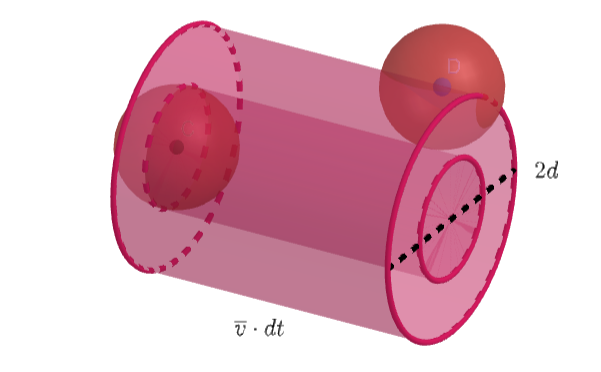
\includegraphics[width=0.7\linewidth]{../images/libero_cammino_medio}
	\caption{Schema del modello adottato per valutare il numero di collisioni medio di una molecola in un intervallo di tempo dt, ipotizzando le altre molecole ferme e di diametro uguale alla prima}
	\label{fig:liberocamminomedio}
\end{figure}
\FloatBarrier
Calcoliamo il volume del cilindro $V_c$ e la frequenza di collisioni, considerando che il numero di molecole con centro all'interno del volume del cilindro è calcolabile moltiplicando questo volume per la densità di molecole nel contenitore del gas, ottenuto con il rapporto $\frac{N}{V_{tot}}$. 
\begin{align*} 
	&V_c = \pi d^2 \overline{v} dt = \sigma \overline{v} dt\\
	&f = \frac{\left(\sigma \overline{v} dt\right)}{dt} \frac{N}{V_{tot}} = \frac{\sigma \overline{v} N}{V_{tot}}\\
\end{align*} 
Dove $\sigma$ è una costante definita come $\sigma \equiv \pi d^2$.\\
Si ottiene che, eliminando le ipotesi semplificative, si ottiene un fattore $\sqrt{2}$ in più, dunque la frequenza diventa
\begin{align*} 
f = \frac{\sigma \overline{v} N}{V_{tot}}\sqrt{2}\\
\end{align*} 
Dall'espressione della frequenza è immediato calcolare il libero cammino medio $\lambda$
\begin{align*} 
	\lambda = \frac{\overline{v}}{f} = \frac{\overline{v} V_{tot}}{\sigma \overline{v} N\sqrt{2}} = \frac{n R \frac{\theta}{p} }{\sigma n N_a \sqrt{2}} = \frac{k_b\theta}{\sqrt{2}\sigma p}
\end{align*} 
Dove $V_{tot}$ è stato sostituito avvalendosi dell'equazione di stato dei gas perfetti, il numero di molecole è stato sostituito con il numero di moli per il numero di Avogadro, infine è stata sostituita la costante di Boltzmann.\\
A titolo d'esempio, il mfp dell'$O_2$ a $300\ K$ e $1\ atm$ è di $\lambda = 300\ \mu m$ mentre la distanza intermolecolare media calcolata in precedenza era 100 volte più piccola. 
\section{Generalizzazione della teoria}
Come visto, il lavoro in meccanica è definito come l'integrale su un percorso del lavoro infinitesimo, il lavoro infinitesimo è invece definito come il prodotto fra la forza e lo spostamento infinitesimo. \'{E} possibile fornire una generalizzazione di questa definizione introducendo innanzitutto i concetti di \textbf{forza generalizzata} e \textbf{spostamento generalizzato}
\begin{definition}[coordinate generalizzate]
	Le coppie forza generalizzata-spostamento generalizzato sono dette coordinate generalizzate (di un sistema fisico) e costituiscono una coppia di generatori dello spazio delle configurazioni (ovvero dei possibili stati che un sistema può assumere). La prima è sempre una grandezza intensiva mentre la seconda estensiva.
\end{definition}
Abbiamo accennato alle coordinate generalizzate o termodinamiche nella prima sezione. A partire da questa definizione possiamo generalizzare anche il concetto di lavoro
\begin{definition}[lavoro generalizzato]
	Il lavoro termodinamico generalizzato infinitesimo è definito come il prodotto fra una forza generalizzata (grandezza intensiva) esercitata dall'ambiente esterno ed uno spostamento generalizzato (grandezza estensiva) infinitesimo.\\
	Il lavoro generalizzato è definito come l'integrale del lavoro infinitesimo. 
	Per convenzione, è positivo se il lavoro è fatto dal sistema e negativo quando è subito (cioè fatto dall'ambiente esterno sul sistema). 
\end{definition}
In un grafico che rappresenti le coordinate generalizzate avremmo che il lavoro è l'area sotto la curva della trasformazione (che congiunge due stati di equilibrio). la forma della curva dipende dal tipo di trasformazione.  
Alcuni esempi di coordinate generalizzate con i rispettivi lavori generalizzati infinitesimi sono sono:
\begin{align*} 
	\text{meccanica: }(F, s)\rightarrow\delta L = F ds\\ 
	\text{pV: }(p, V)\rightarrow\delta L=p dV\\
	\text{torcente: }(\tau, \theta)\rightarrow\delta L=\tau d\theta\\
	\text{elettrico: }(\varepsilon_e, q)\rightarrow\delta L=\varepsilon_edq\\
	\text{magnetico: }(\mu, u)\rightarrow\delta L=\mu du\\
\end{align*} 
Vediamo dunque che esistono diverse categorie di lavoro generalizzato di cui il lavoro meccanico è solo una tipologia. Possiamo distinguere due tipologie di lavoro dal punto di vista macroscopico: quello meccanico, che genera uno spostamento e quello termodinamico che non lo genera, a livello microscopico tuttavia ogni tipo di lavoro è riducibile ad uno spostamento di particelle. Esempi di questa differenza sono:

\begin{table}[h!]
	\begin{center}
		\begin{tabular}{ || c| c ||}
			\hline
			Meccanico & Non meccanico\\
			\hline
			 & Elettrico\\
			Torcente & Magnetico\\
			 pV& Chimico\\
			 & Gravitazionale\\
			\hline
		\end{tabular}
	\end{center}
\end{table}

Concentriamoci ora sul lavoro pV, quello che useremo di più, ricordando che ciò che svolgeremo è generalizzabile a tutti i tipi di lavoro cambiando le coordinate generalizzate.
\subsection{Lavoro pV}
Consideriamo un cilindro adiabatico (isolante termicamente) di volume V pieno di gas a temperatura $\theta$ su cui preme un pistone con pressione p. In questo caso il lavoro generalizzato infinitesimo è definito come la forza generalizzata esercitata dall'ambiente sul sistema cilindro-pistone per lo spostamento infinitesimo da essa provocato. Immaginiamo che il sistema sia immerso nell'aria a pressione di 1 atm e che sul pistone siano poste due masse $m_1$ ed $m_2$. Immaginiamo poi di togliere la massa $m_2$: avremo una pressione esterna iniziale ed una finale
\begin{align*} 
&p_e=p_a+\frac{(m_1+m_2)\cdot g}{S}\\
&p_e'=p_a+\frac{m_1\cdot g}{S}\\
\end{align*} 
La pressione diminuisce dunque il gas si espande e nel farlo muove il pistone verso l'alto contro una forza esterna. Siamo dunque in presenza di lavoro generalizzato, ricaviamo la sua espressione per le coordinate pV a partire dalla definizione meccanica di lavoro (integrale della forza per uno spostamento infinitesimo). 
\begin{align*} 
	&F_e = p_e' S = p_a S + m_1 g\\
	&\delta L = F_e dh\\
	&L= \int_{i}^{f}F_e dh = \int_{i}^{f} p_e' S dh = \int_{i}^{f} p_e' dV = p_e' \Delta V
\end{align*} 
In questo caso la pressione esterna è costante dunque è stato semplice risolvere l'integrale, bisogna tuttavia precisare che in generale l'espressione funzionale di p dipende dal volume e dalla temperatura, dunque se non conosciamo come la temperatura dipenda dal volume e come la pressione dipenda dal volume non sappiamo calcolare l'integrale. Esistono casi particolarmente semplici, come le trasformazioni a temperatura costante, ed è nota la funzione $p(V)$ in cui è immediato calcolare questo integrale.
\begin{align*} 
	&L= \int_{i}^{f} p_e(V,\theta) dV
\end{align*} 
Questa è la forma generale che descrive il lavoro di un sistema idrostatico. Possiamo svincolarci dall'esempio del pistone immaginando un qualsiasi sistema che espandendosi riesca a contrastare la pressione esterna (o contraendosi venga contrastato da essa). In generale è importante sottolineare che \textbf{il lavoro generalizzato è definito in base alla forza esterna}. \\
Se lo spostamento generalizzato avviene gradualmente, per step infinitesimi, la trasformazione sarà quasistatica cioè transita fra stati infinitamente vicini fra loro e quindi approssimabili come di equilibrio. In virtù di ciò, in ognuno di questi stati la pressione esterna e quella interna saranno uguali quindi solo in questo caso potremo sostituire la pressione esterna con quella interna 
\begin{align*} 
	\delta L = p_e dV = (p_e+dp)dv =p_edV + dpdV = p_e dV\simeq p_i dV
\end{align*} 
\textit{Potremo dunque calcolare il lavoro generalizzato come l'integrale della forza generalizzata interna per lo spostamento generalizzato solo se la trasformazione è quasistatica}
\begin{align*} 
	L = \int_{i}^{f}p_i dV
\end{align*} 
\subsection{Calcolo del lavoro in casi semplici}
Vediamo ora alcuni casi semplici in cui è possibile calcolare l'integrale
\begin{enumerate}
	\item Isocòra: V costante, il sistema non effettua alcuno spostamento generalizzato (dV = 0), l'integrale è nullo. 
	\begin{figure}[h!]
		\centering
		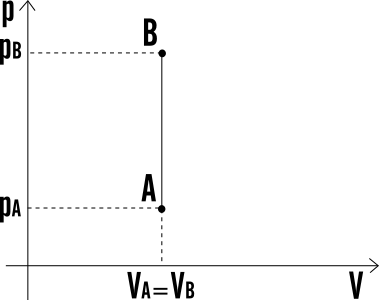
\includegraphics[width=0.4\linewidth]{../images/trasformazione-isocora}
		\caption{Grafico sul piano di Clapeyron di una trasformazione isocora}
		\label{fig:figname}
	\end{figure}
	\FloatBarrier
	\item Isobara: P costante, la trasformazione deve essere quasistatica altrimenti la variazione di volume sarebbe diversa per motivi che vedremo in seguito. Il grafico è semplicemente un segmento dunue calcolare l'aria sottesa è molto semplice. 
	\begin{align}\label{eq:lavoro_pcost}
		L = \int_{v_i}^{v_f}p dV = p\int_{v_i}^{v_f} dV = p\Delta V = p(V_f-V_i) 
	\end{align} 
\begin{figure}[h!]
	\centering
	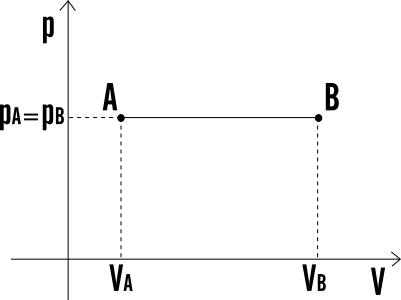
\includegraphics[width=0.4\linewidth]{../images/trasformazione-isobara}
	\caption{Grafico sul piano di Clapeyron di una trasformazione isobara}
	\label{fig:trasformazione_isobara}
\end{figure}
\FloatBarrier
	\item Isoterma con gas perfetto: $\theta$ costante e $p(V) = \frac{nR\theta}{V}$, quasistatica
	\begin{align*} 
		L = \int_{V_i}^{V_f} p(V)dV = \int_{V_i}^{V_f} \frac{nR\theta}{V} dV = n r \theta \int_{V_i}^{V_f} \frac{dV}{V} = n R \theta \ln\left(\frac{V_f}{V_i}\right)
	\end{align*} 
\begin{figure}[h!]
	\centering
	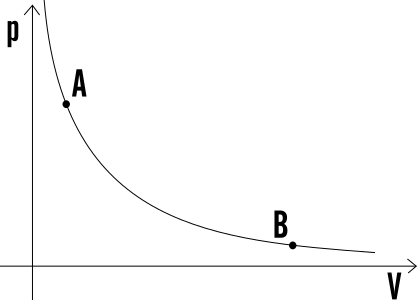
\includegraphics[width=0.5\linewidth]{../images/trasformazione-isoterma}
	\caption{Grafico sul piano di Clapeyron di una trasformazione isoterma}
	\label{fig:trasformazione-isoterma}
\end{figure}
\FloatBarrier
	\item Isoterma con gas reale: $\theta$ costante e $p(v) =\frac{R\theta}{v-b}-\frac{a}{v^2}$, quasistatica
	\begin{align*} 
	&L = \int_{v_i}^{v_f} p(v)dv =\int_{v_i}^{v_f} \left(\frac{R\theta}{v-b}-\frac{a}{v^2}\right) dv = R\theta\int_{v_i}^{v_f} \frac{dv}{v-b}  - a\int_{v_i}^{v_f}\frac{dv}{v^2} =\\
	&R\theta \ln\left(\frac{v_f-b}{v_i-b}\right) + a\left(\frac{1}{v_f}-\frac{1}{v_i}\right)
	\end{align*} 
	Si noti che questa espressione differisce da quella dei gas perfetti per il secondo termine, e per la sottrazione del covolume al primo termine. Il secondo termine riduce sempre il lavoro e rispecchia l'azione delle forze intermolecolari che, essendo attrattive, rallentano le collisioni diminuendo la pressione interna. Per questo il lavoro diminuirà. Si osservi che il lavoro diminuisce sia in compressione che in espansione perchè cambia il segno del secondo termine (in una compressione il secondo termine è positivo mentre il lavoro è negativo, se la pressione diminuisce l'ambiente dovrà fare meno lavoro a parità di compressione).  
	Anche la sottrazione del covolume riduce il lavoro; del punto di vista fisico ce lo spieghiamo perché, essendo il lavoro direttamente proporzionale allo spostamento generalizzato (in questo caso il volume), se la molecola occupa uno spazio finito il volume restante dove espandersi è tanto minore quanto più volume occupano le molecole (la somma dei volumi occupati da tutte le molecole contenute in una mole è proprio il covolume b).
\begin{figure}[h!]
	\centering
	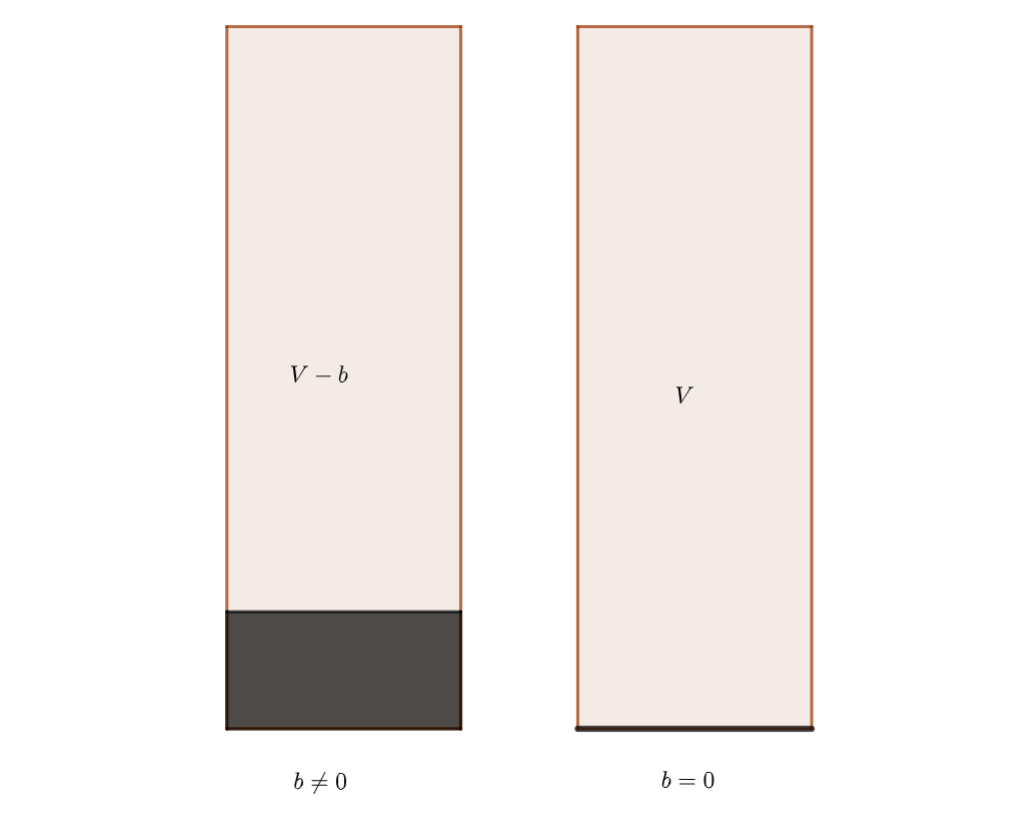
\includegraphics[width=0.6\linewidth]{../images/lavorocovolume}
	\caption{Considerando la regione in nero come la somma dei volumi occupati dalle singole molecole (a sinisttra il caso reale, a destra quello perfetto), risulta chiaro che il volume libero in cui può avvenire lo spostamento è tanto minore quanto è grande il covolume b.}
	\label{fig:lavorocovolume}
\end{figure}
\FloatBarrier
Ne segue che il lavoro di espansione di un gas reale è sempre minore di quello di un gas perfetto.
\item Espansione libera: espansione non-quasistatica in cui il gas si espande liberamente contro una pressione esterna nulla (nel vuoto). Ricordando che il lavoro generalizzato è definito in base alla forza generalizzata esterna (in questo caso la pressione), questo sarà nullo poiché la pressione esterna è pari a zero. 
	\begin{figure}[h!]
		\centering
		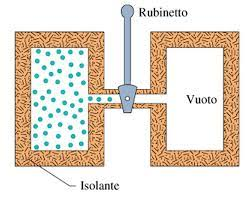
\includegraphics[width=0.5\linewidth]{../images/espansione_libera}
		\caption{Schema dell'espansione libera, inizialmente il rubinetto è chiuso, una volta aperto comincia l'espansione non quasistatica del gas nel vuoto}
		\label{fig:espansione_libera}
	\end{figure}
	\FloatBarrier
	\item Stati condensati: ovvero liquidi e solidi, in cui in generale non si conosce la p(V) ma è possibile comunque calcolare il lavoro con alcune approssimazioni. Cominciamo con l'esplicitare la dipendenza del volume dalla temperatura e dalla pressione per poi scrivere la variazione infinitesima in funzione di essi (scritta come lineare perché qualunque variazione infinitesima è approssimabile a lineare). Sostituiamo poi i valori $\alpha$ e $k$ ottenuti precedentemente e approssimiamo la variazione di temperatura nulla ($d\theta = 0$).  
	\begin{align*} 
		&V = V(\theta, p)\\
		&dV = \left(\frac{\partial V}{\partial \theta}\right)_p d\theta + \left(\frac{\partial V}{\partial p}\right)_{\theta} dp = V(\alpha d\theta-\frac{1}{k} dp)\simeq-\frac{V}{k}dp\\
	\end{align*}  
Sostituiamo quindi il differenziale del volume e consideriamo il volume costante durante la trasformazione poiché negli stati condensati una variazione di volume molto piccola provoca una grande variazione di pressione (volume approssimabile a costante). Infine possiamo calcolare l'integrale definito e ottenere il valore finale della pressione. 
\begin{align*} 
	&L=\int_{i}^{f}pdV = -\int_{p_i}^{p_f}p\frac{V}{k}dp \simeq -\frac{V}{k}\int_{p_i}^{p_f}pdp = -\frac{V}{2k}\left(p_f^2-p_i^2\right)
\end{align*} 
Si noti che se $p_f > p_i$ si ha un lavoro negativo, cioè operato dall'ambiente sul sistema. 
\end{enumerate}
\begin{exercise}
	Un blocco d'acciaio di volume $V = 1\ dm^3$ inizialmente a pressione atmosferica viene compresso con una pressione di $200\ atm$, il modulo di comprimibilità isoterma dell'acciaio è $k = 160\ GPa$. Calcolare il lavoro termodinamico considerando i casi in cui la trasformazione sia quasistatica o brusca.\\
	Cominciamo con il verificare che l'approssimazione a volume costante sia accettabile sfruttando la definizione di k:
	\begin{align*} 
		|\frac{dV}{V}|=|\frac{p}{k}|=\frac{200\ atm}{160\ Gpa}=\frac{200\cdot 1.013\cdot 10^5}{160\cdot 10^9} \simeq 10^{-4} = 0.01 \%
	\end{align*} 
	Cioè in percentuale il volume varia di una percentuale trascurabile. Studiamo ora il caso quasistatico, ovvero quello ricavato nel punto 6 precedente:
	\begin{align*} 
		&L_{qs} = -\frac{V}{2k}\left(p_f^2-p_i^2\right) = -1.28\ J\\	
	\end{align*} 
	Il segno è negativo perché si ha una compressione. Nel caso brusco consideriamo la pressione costante durante la trasformazione, visto che cambia istantaneamente.
	\begin{align*} 
	L_b = p_f\Delta V = p_f\Delta V = p_f\left(-\frac{V}{k}\Delta p \right)=-\frac{V}{k} p_f(p_f - p_i) = -2.55\ J
	\end{align*} 
	Ipotizzando il solido perfettamente elastico, ripetere il calcolo inverso, ovvero se il passaggio avviene da $200\ atm$ a $1\ atm$ ($p_i$ e $p_f$ inversi rispetto a prima).
	\begin{align*} 
		&L'_{qs} = -\frac{V}{2k}\left(p_f^2-p_i^2\right) = +1.28\ J\\
		&L'_b = -\frac{V}{k} p_f(p_f - p_i) = +1.28 \cdot 10^{-2}\ J
	\end{align*} 
	Si noti che, tenendo conto del segno, il lavoro quasistatico è sempre maggiore di quello adiabatico, questo è un risultato completamente generale che vale per ogni tipo di lavoro (non solo quello pV) e che sarà più chiaro grazie al secondo principio della termodinamica.
\end{exercise}
\subsection{Attrito e lavoro}
Spesso nel lavoro pV non è possibile trascurare l'attrito. Se dovessimo tenerne conto avremmo intuitivamente che in un espansione, a parità di spostamento generalizzato il lavoro compiuto sarà maggiore (è come se l'attrito fosse una forza esterna che si oppone nell'espansione). D'altra parte, in una compressione, l'attrito contrasta la forza esterna, è come se fosse una forza interna che si oppone alla compressione dunque avrà segno opposto a quello del lavoro della forza esterna. Riassumendo
\begin{align*} 
	&\text{Espansione: } L = |L_e| + L_a\\
	&\text{Compressione: } L = -|L_e| +L_a
\end{align*} 
\subsection{Circuitazione del lavoro generlizzato}
Dal punto di vista geometrico, rappresentando l' espansione e la compressione sul piano di Clapeyron (per un lavoro pV, ma più in generale su qualsiasi piano che riporti le coordinate generalizzate) il lavoro sarà l'integrale sotto la curva della trasformazione, per convenzione in un espansione l'integrale è positivo e in na compressione negativo. Se avviene una espansione ed una compressione in modo che il punto di arrivo della prima coincida con il punto di partenza della seconda (e vice versa) avremo un ciclo il cui lavoro è definito dall'area all'interno della figura chiusa, se il ciclo è in senso orario per definizione è positivo, se antiorario negativo. 
\begin{definition}[Ciclo termodinamico]
	Si dice ciclo termodinamico o semplicemente ciclo una trasformazione o composizione di trasformazioni che, partendo da uno stato iniziale, alla fine della trasformazione troni a quello stato. Graficamente è rappresentato da una linea chiusa. 
\end{definition}
\begin{figure}[h!]
	\centering
	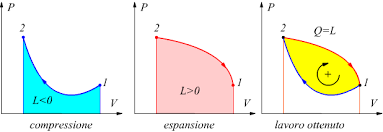
\includegraphics[width=0.5 \linewidth]{../images/ciclo}
	\caption{Grafico di un lavoro generalizzato positivo, uno negativo e la combinazione dei due (un ciclo) in cui il lavoro è dato dall'area della figura chiusa}
	\label{fig:ciclo}
\end{figure}
\FloatBarrier
Il lavoro di un ciclo non è altro che la circuitazione che in generale abbiamo visto essere diversa da zero. Ne segue quindi che in generale un lavoro generalizzato non è conservativo e che un lavoro conservativo è un caso particolare.
%Tensione superficiale e bolla di sapone
\section{Calore e primo principio}
Cominciamo introducendo il lavoro adiabatico, ovvero il lavoro condotto tenendo un sistema all'interno di pareti adiabatiche (ovvero che non permette scambi di energia e materia fra il sistema e l'ambiente esterno). Procediamo illustrando un esperimento: effettueremo trasformazioni adiabatiche concatenate che porteranno da uno stato i ad uno stato f passando per percorsi diversi. Il sistema adottato è un fluido in un cilindro con un pistone.\\
Nel primo caso faremo una compressione adiabatica (da i a 1) e un'espansione isoterma (da 1 a f). 
\begin{align*} 
	L = L_{i1}+L_{1f}= \int_{1}^{i}pdV +[\int_{f}^{1}pdV+mgh]
\end{align*} 
La prima trasformazione è ottenuta semplicemente comprimendo il gas con il pistone mentre la seconda facendolo espandere e riscaldandolo contemporaneamente mediante un apposito apparecchio (ad esempio un mulinello che girando dissipa energia meccanica facendo aumentare la temperatura).\\
nel secondo caso faremo prima un'espansione isoterma (da i a 2) come visto prima e poi aumenteremo la temperatura mantenendo il volume costante. 
\begin{align*} 
	L' = \int_{i}^{2}pdV+mgh'+mgh''
\end{align*} 
Si nota sperimentalmente che $L = L'$, da cui segue che, essendo il lavoro in un percorso chiuso, una trasformazione adiabatica è conservativa! Ne segue che il lavoro in questo caso è una funzione che dipende unicamente dallo stato iniziale e finale del sistema. 
\begin{align*} 
	&\delta L = -dU\\
	&\exists U : L^{(ad)} = -\Delta U = U_i-U_f
\end{align*} 
Possiamo definire una nuova funzione di stato, che chiameremo \textbf{energia interna} U (misurata in Joule). La convenzione di porre il segno negativo serve per far risultare il lavoro positivo se $U_i>U_f$ in modo da poter interpretare il lavoro come una "spesa" di energia interna.\\
Cosa succede se invece il lavoro non è adiabatico (uso pareti che non isolano il sistema)? Confrontiamo quindi una compressione adiabatica (da i ad f) con una compressione isoterma (da i a 1) concatenata ad un aumento di temperatura a volume costante (da 1 a f). Si noti che in quest'ultima trasformazione, visto che il volume non cambia, non abbiamo nessuno spostamento generalizzato dunque il lavoro sarà nullo. 
\begin{align*} 
&L^{(ad)} = \int_{i}^{f} p dV = -dU\\
&L^{(na)} = \int_{i}^{1}pdV+0
\end{align*} 
risulta chiaro che l'integrale da i ad 1 è minore di quello da i ad f dunque si ha
\begin{align*} 
	L^{(na)}<L^{(ad)}
\end{align*} 
Possiamo quindi definire una nuova grandezza fondamentale in termodinamica: il \textbf{calore}.
\begin{definition}[Calore]
	Definiamo calore la differenza tra il Lavoro compiuto in un percorso e il lavoro adiabatico che sarebbe compiuto nel percorso corrispondente. Essendo il lavoro adiabatico conservativo possiamo dare una definizione equivalente scrivendo
	\begin{align*} 
		Q = \Delta U + L
	\end{align*} 
\end{definition}
Quest'ultima formula è la formalizzazione del primo principio della termodinamica
\begin{definition}[Primo principio della termodinamica]
	Durante una qualsiasi trasformazione termodinamica la variazione di energia interna $\Delta U$ è uguale alla differenza tra il calore Q e il lavoro L scambiati con l'ambiente. 
\end{definition}
Svolgiamo alcune considerazioni su quanto visto.
\begin{itemize}
\item Fisicamente il calore può essere visto come l'energia scambiata fra due sistemi in forma diversa dal lavoro. Cioè, la variazione di energia interna di un sistema è data dallo scambio di energia per lavoro (il pistone che si muove ad esempio)  e per scambio di calore.
\item Possiamo ora meglio comprendere il ruolo delle pareti adiabatiche nelle trasformazioni: esse semplicemente non permettono che avvengano scambi di calore con l'ambiente.
\item Introdurre il concetto di calore non fa altro che dare un nome a tutte le energie che in meccanica erano "dissipate", ora sappiamo che queste non vengono perse ma trasformate in calore, che per ora è semplicemente un nome sotto cui cadono tutte le energie dissipate nelle trasformazioni. Ad esempio, l'energia meccanica "dissipata" da una forza d'attrito in realtà viene trasformata in calore. Ciò offre una estensione del principio di conservazione dell'energia meccanica ad un principio che ora diventa una legge di natura: il principio di conservazione dell'energia (L'energia non si crea e non si distrugge ma si trasforma). Per questo motivo la relazione espressa dal primo principio è universale, valida per qualsiasi tipo di trasformazione. 
\item I differenziali $\delta Q$ e $\delta L$ non sono esatti ma $\delta(Q-L)$ lo è perché uguale a $dU$.
\item In realtà la forma più generale del primo principio dovrebbe tener conto di tutte le energie agenti sul sistema che potrebbe ad esempio essere soggetto a campo gravitazionale. La forma più generale è dunque
\begin{align*} 
	Q-L = \delta U + \sum_i \Delta E_i
\end{align*} 
In seguito considereremo sempre sistemi in cui è presente solamente l'energia interna dove quindi il centro di massa è in quiete e quindi l'energia interna coincide con quella interna. 
\item Nonostante il calore nel sistema internazionale si misuri in Joule (essendo omogeneo all'energia e al lavoro) per motivi storici è tutt'oggi in uso un'altra unità di misura, la caloria definita come la quantità di calore necessaria ad aumentare di un grado la temperatura di un grammo d'acqua da 14.5 C a 15.5 C a pressione atmosferica. 
\begin{align*} 
	1\ cal = 4.186\ J
\end{align*} 
\item Il primo principio sancisce l'impossibilità di realizzare il moto perpetuo di prima specie ovvero quello in cui mediante un moto periodico si produce lavoro utile all'infinito senza immettere energia nel sistema. Una macchina periodica (come il motore di una macchina) deve necessariamente compiere un ciclo termodinamico in cui $\Delta U = 0$ poiché U è una funzione di stato che (dipende solo da stato iniziale e finale che sono gli stessi in questo caso). Ne segue per il primo principio che $L = Q$ ovvero che il lavoro prodotto è uguale all'energia immessa nella macchina sotto forma di calore. Il lavoro non può venire dal nulla proprio per il principio di conservazione dell'energia, strettamente legato al primo principio. Con il secondo principio scopriremo che non è neanche possibile trasformare tutto il calore immesso in lavoro utile. 
\end{itemize} 
\subsection{Esempio di applicazione del primo principio}
Riprendiamo l'esempio del blocco e della rampa già visto precedentemente e reinterpretiamolo applicando il primo principio della termodinamica. Sappiamo che la scelta del sistema è arbitraria dunque confrontiamo le varie possibilità. Chiamiamo il sistema della rampa R e quello del blocco B.
\begin{enumerate}
\item $S \equiv B + R$\\
In questo caso stiamo considerando la totalità del sistema, che è per ipotesi isolato dall'ambiente esterno, non ci sarà dunque scambio di calore (Q = 0). L'attrito è considerato interno al sistema, per questo il lavoro sarà fatto solo dal campo gravitazionale ($L = L_g$)
\begin{equation}
	L_g = -\Delta U_{tot} = U_i-U_f < 0
\end{equation} 
Il lavoro è negativo perchè è fatto dall'ambiente sul sistema (si veda la definizione di lavoro termodinamico)
\item $S\equiv B$\\
In questo caso l'attrito sarà esterno al sistema dunque il lavoro ha una componente dovuta alla gravità e una all'attrito. 
\begin{align*} 
	L = L_g + L_a = - \Delta U_b + Q_b
\end{align*} 
\item $S\equiv R$\\
Essendo la rampa ferma rispetto al campo gravitazionale, il suo lavoro sarà nullo (L = 0).
\begin{align*} 
	Q_r = \Delta U_r
\end{align*}  
\end{enumerate}
Vogliamo trovare un'espressione della lavoro d'attrito, basterà sottrarre la somma di quanto ottenuto nel secondo e nel terzo caso con quanto ottenuto nel primo. Abbiamo ottenuto tre proprietà diverse relative allo stesso evento fisico e quindi valide contemporaneamente: mettiamo a sistema e risolviamo per $L_a$.
\begin{align*} 
\begin{cases}
		L_g =  -\delta U_{tot} \\
		L_g + L_a = - \Delta U_b + Q_b\\
		Q_r = \Delta U_r
\end{cases}
\end{align*} 
sappiamo inoltre che $\Delta U_{tot} = \Delta U_b + \Delta U_r$ dunque possiamo scrivere
\begin{align*} 
	&-\Delta U_{tot} + L_a = - \Delta U_b + Q_b\\
	&-\Delta U_b - \Delta U_r+L_a =  - \Delta U_b + Q_b\\
	&- \Delta U_r+L_a =  Q_b\\
	&\Rightarrow L_a =  Q_b + Q_r
\end{align*} 
Quest'ultima relazione è di particolare interesse perché ci fornisce informazioni interessanti sul calore (che va a risolvere la "perdita" d'energia che operava l'attrito nell'ambito della meccanica). Il lavoro d'attrito totale è pari alla totalità del calore scambiato tra gli oggetti.\\
Dal punto di vista microscopico possiamo immaginare un modello molto approssimativo ma efficace: immaginiamo la superficie di contatto scabra fra blocco e rampa con formata da lamelle che vanno a toccarsi quando c'è moto relativo fra i due. L'energia cinetica del corpo che si muove viene trasferita alle lamelle che si mettono ad oscillare, aumentando l'energia cinetica interna del corpo. come abbiamo già visto l'energia cinetica interna non è altro che la temperatura del corpo stesso, che quindi aumenterà. Il lavoro d'attrito non fa altro che trasformare energia cinetica in energia interna (aumenta la temperatura). 
\section{Capacità termica, calore specifico e calore latente}
Come visto, il principio zero ci ha portato ad introdurre la temperatura mentre il primo principio il calore (si noti come queste due grandezze scaturiscono formalmente da questi due principi), volgiamo ora studiare il legame fra queste. Possiamo vedere questa proprietà come \textbf{inerzia termica} (corrispettivo della massa o del momento d'inerzia in meccanica) cioè quella grandezza che si oppone alla variazione di temperatura (come la massa si oppone alla variazione di velocità).  \\
In particolare, vogliamo una quantità che ci dica, a parità di Joule di calore immessi, quanto varia la temperatura. In prima approssimazione potremmo formulare un indice, del tipo
\begin{align*} 
	\overline{C} \equiv \frac{Q}{\theta_f - \theta_i}
\end{align*} 
Tuttavia risulta sperimentalmente che questo $\overline{C}$ dipende dalla temperatura: se la differenza di temperatura è fra 0 e 10 o fra 50 e 60 la quantità di calore per farla avvenire è diversa. Quella che abbiamo definito sarà dunque una proprietà media nell'intervallo ($\theta_f\ , \theta_i$) che chiameremo \textbf{capacità termica media}. \'{E} utile introdurre una grandezza analoga ma puntuale, che chiameremo \textbf{capacità termica}
\begin{align*} 
	C(\theta) \equiv \lim_{\theta_f \to \theta_i} \frac{Q}{\theta_f - \theta_i} = \frac{\delta Q}{d \theta}
\end{align*} 
Il calore non è un differenziale esatto perché definito come somma di lavoro e variazione di energia interna e il lavoro non è un differenziale esatto. Si noti che la dimensione della capacità termica è $\frac{J}{K}$.\\
Tuttavia ciò non basta per avere un indice affidabile, è intuitivamente chiaro che più materiale si ha da riscaldare, più energia sarà necessaria. Vogliamo allora un indice che dipenda o dalla massa o dal numero di moli, definiamo così \textbf{calore specifico} ($c_m$) e \textbf{calore molare} ($c$)
\begin{align*} 
&c_m \equiv \frac{1}{m} \frac{\delta Q}{d\theta}\\
&c \equiv \frac{1}{n} \frac{\delta Q}{d\theta}
\end{align*} 
dove m è la massa del corpo in esame ed n il numero di moli contenute.\\
Infine, risulta che a seconda della modalità con cui è riscaldato il copro avremo che la temperatura varierà in modo diverso a parità di massa (o moli) e di $\Delta \theta$. Introduciamo quindi il calore molare a pressione costante e a volume costante (analogamente potremmo definirle a partire dal calore specifico)
\begin{align*} 
	&c_p \equiv \frac{1}{n} \left(\frac{\delta Q}{d\theta}\right)_p \\
	&c_v \equiv \frac{1}{n} \left(\frac{\delta Q}{d\theta}\right)_V
\end{align*} 
Si noti che, nonostante siano cotanti, le funzioni $c_p$ e $c_v$ dipendono non solo da $\theta$ ma anche rispettivamente dai p e V scelti. 
\begin{align*} 
	&c_p = f(\theta\ , p)\\
	&c_v = f(\theta\ , V)
\end{align*} 
Se il volume rimane costante, il calore non viene trasformato in energia meccanica utile a far muovere il pistone (L = 0) dunque verrà trasformato principalmente in energia interna: farà aumentare la temperatura. Se invece la pressione è costante, ma il pistone è libero di muoversi, una parte di calore sarà trasformata in energia meccanica dunque l'aumento di temperatura sarà minore. Ne deriviamo che vale sempre
\begin{align*} 
	c_p > c_v
\end{align*}  
\begin{exercise}[$c_p$ e $c_v$ di $H_2 O$]
Rappresentando in un grafico $c_m$ su $\theta$ la variazione del calore specifico rispetto alla temperatura, possiamo individuare tre regioni distinte, una in cui si ha lo stato solido una liquido e una gassoso. Risulta che il calore specifico allo stato solido è simile a quello allo stato gassoso ed è circa la metà di quello allo stato gassoso. Se però ci focalizziamo sulla regione allo stato liquido, notiamo che non è costante ma è del tipo
\begin{figure}[h!]
	\centering
	\includegraphics[width=0.7\linewidth]{"../images/calore specifico acqua"}
	\caption{Grafico $c_m$ su $\theta$ per $H_2O$ allo stato liquido. Presenta un minimo a 35 \textdegree C.}
	\label{fig:calore-specifico-acqua}
\end{figure}
\FloatBarrier
\end{exercise}
\subsection{Calore latente}
Spesso accade che un trasferimento di calore risulti in un aumento di temperatura, si potrebbe inferire che il calore genera sempre aumenti di temperatura. Questo è falso e ne vediamo un esempio di seguito.\\
\begin{figure}[h!]
	\centering
	\includegraphics[width=0.6\linewidth]{"../images/calore specifico acqua(1)"}
	\caption{Grafico temperatura su tempo per l'$H_2 O$. Le regioni a temperatura costante sono quelle in cui avviene il cambio di fase.}
	\label{fig:calore-specifico-acqua1}
\end{figure}
\FloatBarrier
Questo grafico smentisce l'ipotesi iniziale: ci sono regioni in cui la temperatura non cambia, cosa succede? Durante un cambiamento di stato, ad esempio da solido a liquido, l'energia del calore non viene trasformata in energia interna ma viene usata per rompere i legami che legano le molecole di $H_2O$ nella struttura cristallina del ghiaccio per farla cambiare di stato. Ne risulta che in una regione, fino a quando il ghiaccio non si scioglie, la temperatura rimane costante (analogamente per l'evaporazione). Il calore necessario per far avvenire il passaggio di stato, a parità di massa, chiaramente dipende dal tipo di materiale preso in considerazione (perché dipende dal tipo di legami da spezzare);  Il calore necessario per effettuare il passaggio di stato di un grammo di una sostanza è detto \textbf{calore latente}.
\begin{align*} 
	&Q_{latente} = m \lambda
\end{align*} 
 Esisteranno un calore latente di fusione ($\lambda_f$) per il passaggio solido-liquido e uno di vaporizzazione ($\lambda_v$) per il passaggio liquido-vapore. In particolare per l'acqua
\begin{align*} 
	&\lambda_f(H_2O) = 333 \frac{J}{g} \\
	&\lambda_f(H_2O) = 2260 \frac{J}{g} 
\end{align*} 
Durante il passaggio di fase la pressione rimane costante (come visto nella correzione di Maxwell dei grafici di Van der Waals, figura (\ref{fig:calcolo-di-maxwell})) dunque varierà solo il volume. Ricordando la (\ref{eq:lavoro_pcost}), il lavoro a pressione costante del passaggio di fase sarà
\begin{align*} 
	&L_{l-v} = p(v_v-v_l)\\
	&L_{s-l} = p(v_l-v_s)
\end{align*} 
dove la prima è il lavoro nel passaggio liquido-vapore e la seconda solido liquido. Tutte le v sono volumi molari e i vari pedici indicano il volume caratteristico prima e dopo della transizione di fase. Ad esempio, i valori del volume prima e dopo del segmento ottenuto con il metodo di Maxwell (Figura (\ref{fig:vanderwaals})) nel grafico di Van der Waals sono $v_v$ e $v_l$.
\begin{exercise}
Una persona prepara del té freddo mescolando $m_t = m_g =520$ g di té caldo (sostanzialmente acqua) con un’uguale quantità di ghiaccio a 0 \textdegree C. Calcolare la temperatura finale di equilibrio $\theta_e$ e l’eventuale massa di ghiaccio restante $m_g'$, se la temperatura iniziale è pari a a)$\theta_i = 90.0$ \textdegree C oppure b) $\theta_i = 70.0$ \textdegree C.\\
Bisogna tenere conto di due possibilità: se $\theta_i$ è abbastanza grande da sciogliere tutto il ghiaccio o se $\theta_i$ non è sufficiente e rimane del ghiaccio non sciolto. Abbiamo infatti due tendenze contrapposte: quella dell'acqua che vuol squagliare il ghiaccio  e quella del ghiaccio che vuole portare l'acqua alla sua temperatura, ovvero 0 \textdegree C. Dobbiamo dunque calcolare il calore necessario perché il ghiaccio si sciolga completamente ($Q_g$) e quello necessario per far arrivare a 0 \textdegree C tutta l'acqua ($Q_t$). Chiaramente $Q_t$ è minore di zero perché per passare da una temperatura maggiore di zero a zero bisognerà "togliere" calore all'acqua. Se, in valore assoluto, serve più calore per portare l'acqua a 0 \textdegree C rispetto a squagliare il ghiaccio, allora questo si scioglierà del tutto. 
\begin{align*} 
	&|Q_t| > |Q_g|\\
	&Q_t = m_t c_m \Delta\theta = m_t c_m (\theta_0-\theta_i)\\
	&|Q_t| =  m_t c_m (\theta_i-\theta_0) = m_t c_m \theta_i\\
	&Q_g = |Q_g| = m_g \lambda_f\\
	&m_t c_m \theta_i >m_g \lambda_f\\
	&\Rightarrow \Delta\theta > \frac{\lambda_f}{c_m} = \frac{333 \cdot 10^3}{4.186 \cdot 10^3} = 79.5 °C
\end{align*} 
Dunque se si verifica $\Delta\theta = \theta_i >79.5$ \textdegree C allora il ghiaccio si scioglie totalmente.
\begin{itemize}
\item[a.] Poiché $\theta_i>79.5$ \textdegree C il ghiaccio si scioglie completamente. Possiamo scrivere la somma di tutti i calori scambiati, che dovrà essere pari a zero visto che il sistema del bicchiere pieno di té è isolato dall'ambiente. 
\begin{align*} 
	&m_t c_m (\theta_e-\theta_i) + m_g \lambda_f + m_g c_m (\theta_e-\theta_0)= 0\\
	&\Rightarrow \theta_e = \frac{1}{2}\left(\theta_i-\frac{\lambda_f}{c_m}\right) = \frac{90-\frac{333}{4.187}}{2} = 5.2 °C\\
\end{align*} 
dove i termini sono rispettivamente: il calore necessario per raffreddare l'acqua da $\theta_i$ a $\theta_e$ (< 0 perché si raffredda), il calore necessario per far squagliare il ghiaccio e il calore necessario per portare a $\theta_e$ il ghiaccio sciolto (inizialmente a temperatura $\theta_0$).
\item[b.] Poiché $\theta_i<79.5$ \textdegree C il ghiaccio non si scioglie completamente, la temperatura d'equilibrio sarà a 0 \textdegree C. Procedendo analogamente a come fatto otteniamo
\begin{align*} 
	&(m_g-m_g') \lambda_f +m_t c_m (\theta_0-\theta_i) = 0\\
	&mg' = \frac{m_t c_m 8\theta_0-\theta_i+mg\lambda_f}{\lambda_f} = \frac{520\cdot 4.187 \cdot(-70)+520\cdot 333}{333} = 62.3 g
\end{align*} 
\end{itemize}
\begin{figure}[h!]
	\centering
	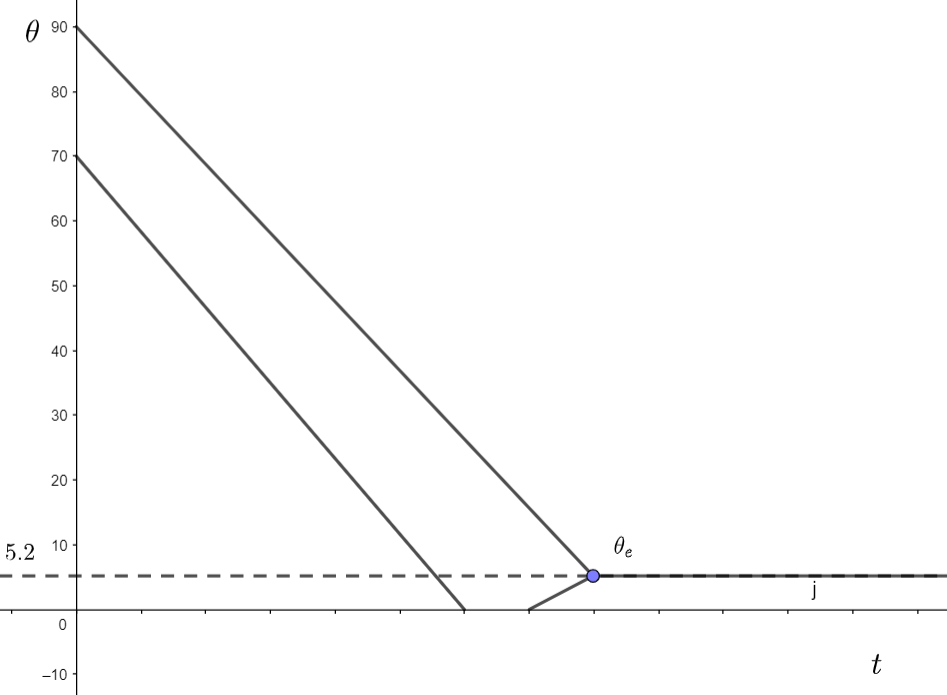
\includegraphics[width=0.6\linewidth]{../images/te_ghiaccio}
	\caption{Grafico comparativo della temperatura in funzione del tempo nei due casi a e b.}
	\label{fig:teghiaccio}
\end{figure}
\FloatBarrier
\end{exercise}
\subsection{Calcolo della temperatura d'equilibrio di sistemi a contatto}
Si considerino due sistemi $S_1$ ed $S_2$ a contatto diatermico rispettivamente di temperatura e capacità $\theta_1\ , C_1$ e  $\theta_2\ , C_2$. Dando per scontato che esista l'equilibrio termico, vogliamo trovare un'espressione della temperatura all'equilibrio $\theta_e$ in funzione delle capacità e temperature iniziali. Cominciamo con il considerare come sistema l'unione dei due sistemi, lo scambio di calore ed il lavoro saranno nulli perchè questi sono isolati dall'esterno e non avviene nessuno spostamento. 
\begin{align*} 
&S \equiv S_1 + S_2\\
&Q = 0\;\quad L=0\ ; \quad \Rightarrow \Delta U_{tot} = 0\\
\end{align*} 
Se consideriamo ora i sistemi singolarmente abbiamo sempre che il lavoro è nullo perché non avvengono spostamenti ma il calore verrà scambiato dunque
\begin{align*} 
&S \equiv S_1 \Rightarrow \Delta U_1 = Q_1\\
&S\equiv S_2 \Rightarrow  \Delta U_2 = Q_2
&\Rightarrow 
\end{align*} 
Visto che la variazione di energia totale deve essere uguale alla somma delle singole variazioni interne abbiamo
\begin{align*} 
&\Delta U_{tot} = \Delta U_1 + \Delta U_2 = Q_1+Q_2 = 0\\
&\Rightarrow Q_1 = -Q_2 
\end{align*}  
Questo è ciò che davvero ci dice il primo principio della termodinamica: il calore assorbito da un sistema deve essere lo stesso ceduto dall'altro. Si noti che fin ora non abbiamo nessuna indicazione sulla direzione del trasferimento di calore, teoricamente il calore potrebbe fluire sia dal sistema caldo a quello freddo sia in verso contrario (questo problema verrà risolto dall'introduzione del secondo principio). Possiamo dunque esprimere il calore in funzione di C e $\theta$ per poi applicare quanto trovato
\begin{align*} 
&\begin{cases}
	Q_1 = C_1 (\theta_e-\theta_1)\\
	Q_2 = C_2 (\theta_e-\theta_2)
\end{cases}\\
&\Rightarrow C_1 (\theta_e-\theta_1) + C_2 (\theta_e-\theta_2) = 0\\
&\Rightarrow \theta_e = \frac{C_1\theta_1+C_2\theta_2}{C_1+C_2} =  \frac{n_1 c_1\theta_1+n_2 c_2\theta_2}{c_1 + c_2}
\end{align*} 
La temperatura di equilibrio si ottiene dalla media pesata delle capacità termica con peso la temperatura iniziale.\\
Se $c_1>>c_2$, risolvendo il sistema otteniamo
\begin{align*} 
	\theta_e = \left(\frac{1+\frac{c_2\theta_2}{c_1\theta_1}}{1+\frac{c_2}{c_1}}\right)\theta_1 \to \theta_1
\end{align*} 
In questo caso il sistema con $c_1$ porta alla sua temperatura il sistema $S_2$ a contatto con esso: abbiamo ottenuto un \textbf{calorimetro}.\\
Si noti l'analogia con gli urti fra punti materiali visti in meccanica: il caso del calorimetro è analogo all'urto di un punto materiale con la parete: come il sistema $S_1$ ha una capacità termica infinita così la parete ha una massa infinita (chiaramente in prima approssimazione e relativamente al sistema con cui interagisce).
\subsection{Calorimetria: misura di $c_m$}
\subsubsection*{Calorimetro di Bunsen (a ghiaccio)}
Il calorimetro di Bunsen è costituito da un tubo di vetro A, a pareti sottilissime, saldato ad un tubo di vetro di diametro maggiore B, il quale termina inferiormente con un tubo pure di vetro di piccolo diametro C piegato due volte ad angolo retto. Nella parte superiore del tubo C si può innestare, a perfetta tenuta, un tubo sottile R graduato. Si riempie apparecchio in parte con acqua distillata, e in parte con mercurio. Il mercurio deve anche occupare parte della vaschetta superiore, il tuo graduato R indica il volume del mercurio.
\begin{figure}[h!]
	\centering
	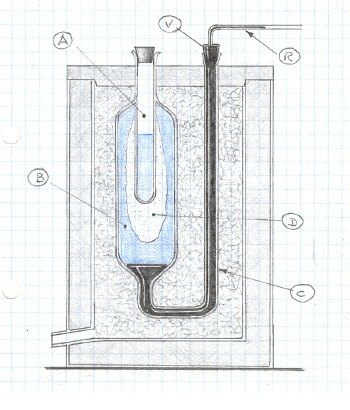
\includegraphics[width=0.5\linewidth]{../images/calorimetro_bunsen}
	\caption{Schema del calorimetro di Bunsen}
	\label{fig:calorimetrobunsen}
\end{figure}
\FloatBarrier
Dopo aver collocato l’apparecchio così preparato in un recipiente contenete del ghiaccio a 0 \textdegree C, in modo che l’acqua ed il mercurio siano portati alla temperatura di 0°C, è necessario procedere alla solidificazione dell’acqua contenuta nel calorimetro. Per questo si versa nel tubo interno A dell’etere, in questo modo l’acqua solidifica (D) e nell’atto della solidificazione il mercurio viene spinto dal tubo B nella vaschetta V per l’aumento di volume del ghiaccio rispetto all'acqua. Quando quasi tutta l’acqua presente nel calorimetro si è solidificata, si toglie l’etere, si versa nel tubo A una piccola quantità di acqua a 0 °C e si tappa il tubo. Si lascia stabilizzare il calorimetro affinché tutto l’apparecchio raggiunga l’equilibrio termico a 0°C. Raggiunta questa condizione, si registra il volume del mercurio ($V_0$).\\
Preparato così l’apparecchio si riscalda il corpo di cui si cerca il calore specifico alla temperatura $\theta$ e lo si inserisce nell’acqua contenuta nel tubo A del calorimetro. Il calore ceduto dal corpo nel passare da $\theta$ a 0°C provoca la fusione di una certa quantità di ghiaccio e, poiché nella fusione del ghiaccio diminuisce il volume, il mercurio diminuirà di volume passando da $V_0$ a $V_1$ che raggiungerà quando tutto l’apparecchio sarà tornato in equilibrio termico a 0 °C.\\
\'{E} chiaro che il volume di cui si è contratto il ghiaccio per quella porzione che si è fusa è uguale a $\delta V = V_1-V_0$, e questa contrazione sarà proporzionale al ghiaccio fuso e quindi anche alla quantità di calore ceduta dal corpo. Si vuole conoscere dalla contrazione il la massa $m_g$ del ghiaccio fuso. Noto il peso specifico del ghiaccio a 0°C = 0,91674 ed il peso specifico dell’acqua a 0°C = 0,99987 si ha:
\begin{align*} 
	\Delta V = \frac{m_g}{0.91674}-\frac{m_g}{0.99987}
\end{align*} 
Da cui è possibile ricavare $m_g$, essendo stato misurato $\Delta V$. Infine, sapendo che il calore necessario per fondere la massa $m_g$ di ghiaccio è uguale al calore trasferito dall'oggetto di cui si vuole misurare $c_m$ (contenuto nel bulbo A) al bulbo B.
\begin{align*} 
&m_g \lambda_f = c_m m \Delta\theta\\
&\Rightarrow c_m = \frac{m_g \lambda_f}{m \Delta \theta}
\end{align*} 
Dove m è la massa dell'oggetto di cui si vuole misurare $c_m$, $\Delta \theta$ è la differenza di temperatura fra l'oggetto in esame e l'acqua (a 0 \textdegree C). Si noti che la misura è tutta basata sul cambiamento di volume dell'acqua da solido a liquido, che deve essere conosciuto con precisione; La variazione di volume a 0 \textdegree C di 1 g di acqua a pressione atmosferica è  $\Delta V_{sl} = 0.0907\ cm^3$.
\subsection*{Calorimetro di Regnault (o delle mescolanze)}
Data una massa $m_a$ di acqua a temperatura $\theta_a$ e calore specifico $c_a$ noti all'interno di un recipiente adiabatico. Si inserisce un corpo, di massa m e temperatura $\theta$ note e calore specifico c da determinare. Dopo una quantità di tempo acqua e corpo arriveranno all'equilibrio termico $\theta_e$, che misuriamo.
\begin{figure}[h!]
	\centering
	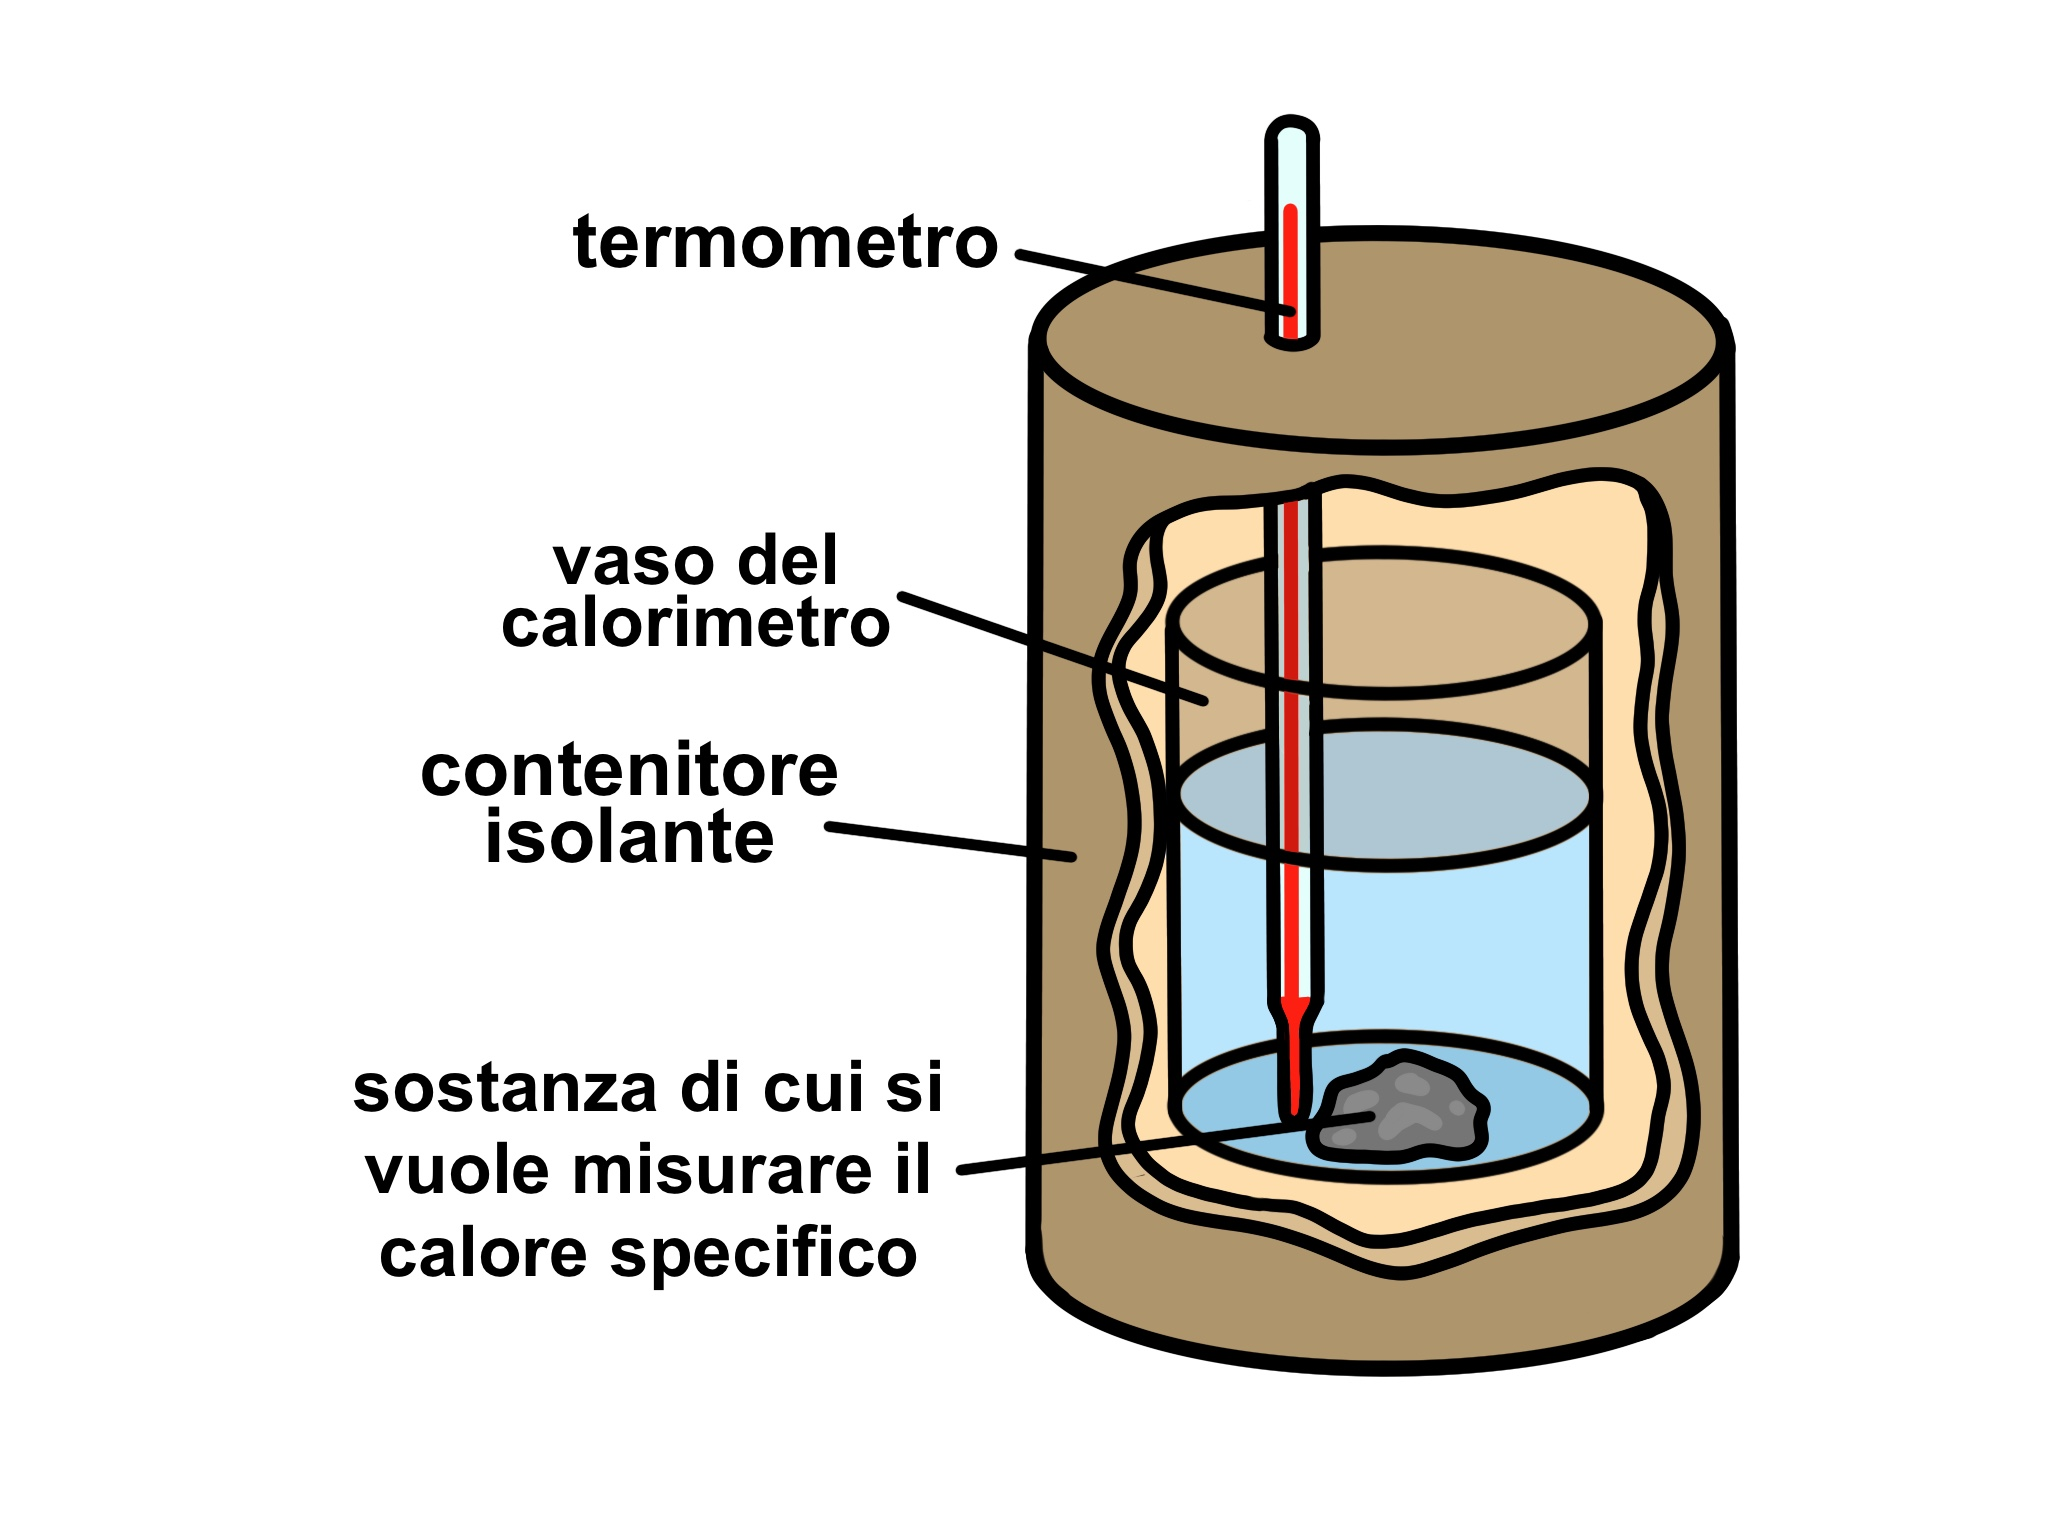
\includegraphics[width=0.5\linewidth]{../images/calorimetro_regnault}
	\caption{Schema esemplificativo del calorimetro di Regnault}
	\label{fig:calorimetroregnault}
\end{figure}
\FloatBarrier
Imponendo che la somma dei calori scambiati deve essere nulla (perchè il sistema è isolato) si ha
\begin{align*} 
&Q_1 + Q_2 = m c \left(\theta - \theta_e\right) + m_a c_a \left(\theta_a - \theta_e \right) \\
&\Rightarrow c = c_a \frac{m_a}{m}\left[\frac{\theta_e - \theta_a}{\theta - \theta_e}\right]
\end{align*} 
Questo esperimento è basato sull'assunto che il recipiente sia perfettamente adiabatico, visto che tali recipienti non esistono si avrà sempre una quantità di calore, per quanto piccola, assorbita da esso. Per migliorare la misura calcoliamo la \textbf{massa equivalente in acqua} da aggiungere per poter assumere il recipiente perfettamente adiabatico. Per calcolala facciamo una taratura prima di effettuare la misura. Consideriamo il recipiente con dell'aqua all'interno di massa \(m_a\), a temperatura \(\theta_a\) e di calore specifico \(c_a\), aggiungiamo un' ulteriore massa \(m_a'\) d'acqua a temperatura\(\theta_a'\) e di calore specifico uguale; dopo un certo intervallo di tempo il sistema raggiungerà la temperatura all'equilibrio \(\theta_e\) che misuriamo. Per tener conto della non perfetta adiabaticità del recipiente, aggiungiamo al computo della somma dei calori la presenza di un'ulteriore massa \(m^*\) d'acqua a temperatura \(\theta_a\) che ci dovrebbe essere se il recipiente fosse perfettamente adiabatico, per raggiungere la $\theta_e$ che effettivamente si misura. 
\begin{align*} 
	c_a m_a (\theta_a-\theta_e)+c_a m_a'(\theta_a'-\theta_e)+c_a m^*(\theta_a-\theta_e) = 0
\end{align*} 
da cui è possibile ricavare la \(m^*\) caratteristica del recipiente usato.\\
Rieffettuare la misura del calore specifico tenendo conto di \(m*\) offre un risultato più preciso. 
\section{Legame fra energia interna e calore molare}
Consideriamo l'energia interna di un sistema idrostatico, sappiamo per le considerazioni svolte nelle sezioni precedenti che la temperatura in realtà è energia interna, ne deduciamo che l'energia interna dipende dalla temperatura. Visto che in un siffatto sistema pV abbiamo solamente due variabili indipendenti dunque la seconda può essere o p o V. consideriamo i due casi in cui una delle due resta costante.
\begin{itemize}
	\item[a)] V = costante\\
	\begin{align*} 
	&\delta Q = dU + pdV\\
	&U = U(\theta\ ,\ V)\\
	&dU = \left(\frac{\partial U}{\partial \theta}\right)_V d\theta +\left(\frac{\partial U}{\partial V}\right)_{\theta} dV\\
	&\Rightarrow \delta Q = \left(\frac{\partial U}{\partial \theta}\right)_V d\theta +\left[\left(\frac{\partial U}{\partial V}\right)_{\theta}+p\right]dV
	\end{align*} 
	ma essendo il volume costante \(dV = 0\) dunque il secondo termine si elimina e rimane
	\begin{align*} 
	\delta Q = \left(\frac{\partial U}{\partial \theta}\right)_V d\theta \Rightarrow \left(\frac{\delta Q}{d \theta}\right)_V = \left(\frac{\partial U}{\partial \theta}\right)_V
	\end{align*} 
	Ricordando la definizione di \(c_v\) possiamo scrivere
	\begin{align*} 
		c_v = \frac{1}{n} \left( \frac{\delta Q}{\partial \theta}\right)_V = \frac{1}{n} \left(\frac{\partial U}{\partial \theta}\right)_V
	\end{align*} 
	\item[b)] p = costante\\
	\begin{align*} 
		&U = U(\theta\ ,\ p) \quad V = V(\theta\ ,\ p)\\
		&\delta Q = dU + pdV\\
	\end{align*} 
	In questo caso il volume non è costante e avremo del lavoro che è energia trasformata, ne dovremo tener conto nell'espressione dell'energia interna (nel caso a V era costante dunque L = 0). Dobbiamo dunque tener conto non solo di dU ma anche di dV.
	\begin{align*} 
		&V = V(\theta\ ,\ p) \quad dV = \left( \frac{\partial V}{\partial \theta}\right)_p d\theta + \left( \frac{\partial V}{\partial p}\right)_{\theta} dp\\
		&\delta Q = \left[\frac{\partial U}{\partial \theta} + p \frac{\partial V}{\partial \theta}\right]d\theta + \left[\frac{\partial U}{\partial p}+ p \frac{\partial V}{\partial p} \right]dp\\
		&\delta Q = \left[\frac{\partial U}{\partial \theta} + p \frac{\partial V}{\partial \theta}\right]d\theta\\
		&\Rightarrow \left(\frac{\delta Q}{d \theta}\right)_p = \left[\left(\frac{\partial U}{\partial \theta}\right)_p + p \left(\frac{\partial V}{\partial \theta}\right)_p\right]
	\end{align*}  
	Considerando la definizione di \(c_p\) possiamo scrivere
	\begin{align*} 
		&c_p = \frac{1}{n}\left(\frac{\delta Q}{d\theta}\right)_p = \frac{1}{n} \left[\left(\frac{\partial U}{d \theta}\right)_p + p \left(\frac{\partial V}{d \theta}\right)_p\right]
	\end{align*} 
\end{itemize} 
Possiamo ora introdurre una nuova variabile di stato in modo da avere espressioni simmetriche di \(c_p\) e \(c_v\) (la ricerca di simmetrie ripaga spesso in fisica e questa nuova grandezza risulterà utile in seguito)
\begin{align*} 
	H \equiv U + pdV
\end{align*} 
questa è chiaramente una variabile di stato perché somma di variabili di stato; notiamo inoltre che è estensiva poiché U lo è ed anche V e il prodotto di una variabile estensiva per una intensiva risulta ancora in una variabile estensiva. Chiamiamo la variabile H \textbf{entalpia}. Intuitivamente, quello che rappresenta U a volume costante lo rappresenta H a pressione costante (questa è la simmetria). Per la teoria dei differenziali, dH è
\begin{align*}  
	&dH = dU + pdV + Vdp \\
	&(dH)_p = dU + pdV = (\delta Q)_p
\end{align*}  
come ci aspettavamo, il differenziale dell'entalpia a pressione costante è uguale a quello del calore a pressione costante. Possiamo dunque riscrivere \(c_p\) come
\begin{align*}  
	c_p = \frac{1}{n} \left(\frac{\partial H}{\partial \theta}\right)_p
\end{align*}  
Questi risultati torneranno utili in seguito per trovare l'espressione funzionale dell'energia interna. 
\subsection{Esperimento di Joule}
Sappiamo che l'energia interna U dipende da temperatura e volume (o pressione e volume, la scelta è arbitraria), vogliamo trovare l'espressione di questa funzione nel caso semplice di un gas perfetto per poi passare a quello reale. Si consideri un recipiente adiabatico all'interno del quale è presente un sistema di due bulbi collegati da un tubo e divisi da un setto inizialmente chiuso, dentro un bulbo è presente un gas molto rarefatto (in condizioni di gas perfetto); il tutto circondato da acqua. Inizialmente il sistema è in equilibrio termico a temperatura $\theta_i$.
Ancor prima di effettuare l'esperimento, per il primo principio sappiamo che, essendo il recipiente adiabatico, non vi sono scambi di calore con l'esterno ed essendo l'espansione libera (nell'altro bulbo c'è il vuoto) il lavoro è nullo. 
\[Q = 0\ ; \quad L = 0\ \Rightarrow U_f = U_i\]
Se ora apriamo il setto avremo un'espansione libera del gas, ci chiediamo se vi sia una variazione di temperatura a seguito dell'espansione. Si nota sperimentalmente che la temperatura non cambia
\[\theta_f )= \theta_i\]
\begin{figure}[h!]
	\centering
	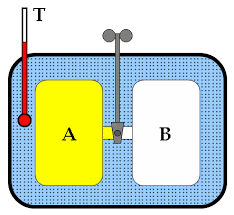
\includegraphics[width=0.5\linewidth]{../images/esperimento_Joule}
	\caption{Schema dell'esperimento di Joule. La temperatura resta invariata a seguito dell'espansione.}
	\label{fig:esperimentojoule}
\end{figure}
\FloatBarrier
Combinando quanto ottenuto possiamo scrivere
\[U_f(\theta\ ,\ V_f) = U_i(\theta_i\ ,\ V_i)\]
Nonostante il volume sia cambiato l'energia interna è rimasta la stessa, ne deduciamo che U, nel caso di un gas perfetto non dipende da V. Se avessimo considerato la dipendenza dalla pressione invece che dal volume avremmo ottenuto che, nonostante la variazione di pressione prima e dopo l'espansione, U non cambia dunque non dipende neanche da p. Se ne deduce che U dipende solo dalla temperatura.\\
Possiamo rivedere la formula appena ottenuta di \(c_v\) in quanto ora sappiamo che la derivata di U rispetto a $\theta$ non è più parziale ma totale
\[c_v =\frac{1}{n}\left(\frac{\partial U}{\partial\theta}\right)=\frac{1}{n}\left(\frac{dU}{d\theta}\right)\]
Possiamo esplicitare il differenziale dell'energia interna da quest'ultima espressione ed integrare ambo i membri per trovare l'espressione funzionale dell'energia in terna rispetto alla temperatura per un gas perfetto.
\begin{align}\label{eq:U_gas_perfetti}
	&\int dU = \int n c_v d\theta\nonumber\\
	&U(\theta) = n c_v \theta + cost.
\end{align} 
A breve discuteremo la costante additiva appena ottenuta.
\subsection{Correzione per i gas reali}
Se il gas non fosse perfetto non dipenderebbe solo da $\theta$ ma anche da V perché non avremmo più solo energia cinetica ma anche energia potenziale, dovuta alle interazioni intermolecolari. Consideriamo nuovamente l'esperimento di Joule, anche se all'interno del bulbo ci fosse un gas reale, il primo principio continuerebbe ad essere valido e avremmo sempre\(\Delta U = 0\). Se a seguito dell'apertura del setto il volume in cui è contenuto il gas aumenta, la distanza media fra le molecole (r) aumenterà. Considerando il grafico di Lennard-Jones notiamo che all'aumentare di r aumenta anche l'energia potenziale (considerando anche il segno, diventa meno negativa) ma visto che l'energia interna deve rimanere costante ciò significa che l'energia cinetica dovrà diminuire. Se però la temperatura e l'energia cinetica sono essenzialmente la stessa cosa, allora anche la temperatura dovrà diminuire. Ne segue che in un gas reale l'energia interna dipende sia dalla temperatura che dal volume (\(U = U(\theta\ ,\ V)\)). 

\begin{align*} 
	dU = \left(\frac{\partial U}{\partial \theta}\right)_V d\theta + \left(\frac{\partial U}{\partial V}\right)_p dV = n c_v d\theta +\left(\frac{\partial U}{\partial V}\right)_{\theta dV}
\end{align*} 

Dove il primo membro è stato sostituito con quanto ottenuto precedentemente per i gas perfetti.\\
\'{E} necessario anticipare una relazione che dimostreremo in seguito che esprime la \textbf{seconda equazione dell'enrgia}
\[ \left(\frac{\partial U}{\partial V}\right)_{\theta} = \theta \left(\frac{\partial p}{\partial \theta}\right)_v - p \]
Questa è valida per una singola mole dunque restringiamo la trattazione ad una mole per poi tornare infine al caso generale.\\
Per l'equazione dei gas reali sappiamo l'espressione di p in funzione di V e \(\theta\), possiamo derivarla rispetto a $\theta$ per poi sostituirla nella seconda equazione dell'energia. 

\begin{align*} 
	&p = \frac{R\theta}{v-b}-\frac{a}{v^2}\\
	&\left(\frac{\partial p}{\partial \theta}\right)_v = \frac{R}{v-b}\\
	&\Rightarrow dU = c_v d\theta + \left[ \theta \left(\frac{R}{v-b}\right)-p \right]dV
\end{align*} 

Possiamo sostituire nuovamente l'espressione della pressione di un gas reale in quest'ultima equazione per ottenere

\begin{align*} 
	dU = c_v d\theta + \left[\frac{\theta R}{v-b}-\frac{\theta R}{v-b}+\frac{a}{v^2}\right] dV = c_v d\theta +\frac{a}{v^2}dV
\end{align*} 

Si noti che, nel caso dell'esperimento di Joule con il gas perfetto, essendo \(dU = 0\), visto che sia \(c_v\) che \(\frac{a}{v^2}\) sono maggiori di zero, se il volume cresce la temperatura deve diminuire (come ottenuto dalle considerazioni sul grafico di Lennard-Jones).\\
Integrando ambo i membri otteniamo l'espressione funzionale dell'energia interna rispetta a temperatura e volume per un gas perfetto. 
\[U(\theta\ ,\ v) = c_v\theta - \frac{a}{v^2}+ cost.\]
Possiamo riaggiungere la variabile del numero di moli (con considerazioni dimensionali otteniamo che al secondo termine deve essere \(n^2\))
\[U(\theta\ ,\ v) = n c_v\theta - \frac{a n^2}{v^2}+ cost.\]
Si noti che in questa espressione compare solo la costante, tipica di ogni gas perfetto, a e non b; ciò è dovuto al fatto che a è il termine correttivo per la presenza di interazioni intermolecolari (rilevanti nel computo dell'energia interna) mentre b è il covolume, che non influenza l'energia interna. Per a che tende a zero si ottiene\( U(\theta)\) per i gas perfetti. Le espressioni precedenti hanno una validità molto ridotta, infatti se la temperatura fosse lo zero assoluto avremmo che l'energia interna sarebbe \(-\frac{a}{v^2}+cost.\), che non ha senso dal punto di vista fisico (oltre che un gas non sarebbe più tale allo zero assoluto). 
\subsection{Energia interna per gas monoatomici, biatomici e poliatomici}\label{sec:energia_interna_mono_bi_poli}
Possiamo vedere l'energia interna dal punto di vista microscopico come la somma dell'energia cinetica delle singole molecole, se ci sono molte molecole questa sarà pari all'energia cinetica media, di cui abbiamo già ricavato un'espressione precedentemente. 

\begin{align*} 
	&U = \sum_i \varepsilon_i= N_a \overline{\varepsilon} = N_a \frac{3}{2} k \theta = \frac{3}{2}n R \theta\\
	&c_v = \frac{1}{n}\left(\frac{dU}{d\theta}\right)_v=\frac{3}{2}R\\
	&\Rightarrow U = n c_v\theta
\end{align*} 

Si noti che abbiamo ricavato una nuova forma macroscopica dell'energia interna, passando per l'approccio microscopico, in cui non è presente la costante additiva risultante dall'integrale nel primo metodo. Ne deduciamo che, per l teoria cinetica dei gas, l'energia di un gas a zero gradi è nulla (sostituendo $\theta=0$). Oggi sappiamo, a fronte dell'approccio quantistico, che in realtà è impossibile avere una energia interna (e dunque un movimento) totalmente assente perché al minimo ci saranno sempre energie dovute all'incertezza inevitabile dovuta al principio d'indeterminazione. Il $c_p$ risulta essere invece \(\frac{5}{2}R\), si definisce infine $\gamma=\frac{c_p}{c_v}=\frac{5}{3}$.\\
La trattazione svolta fin ora è valida solamente per gas perfetti monoatomici, se osserviamo molecole più complesse si nota che questi valori aumentano, in particolare per molecole biatomiche si ha
\[c_v=\frac{5}{2}R\;\quad c_p=\frac{7}{2}R\ ; \quad \gamma = \frac{7}{5}\]
Come ci spieghiamo questo fenomeno? Ricordando la funzione di energia cinetica interna (\ref{eq:energiacinetica_d.o.f.}) notiamo che, ripercorrendo i passaggi con cui abbiamo ottenuto $c_v$ e $c_p$, possiamo tener conto dei gradi di libertà.
\begin{align*} 
	&U = N_a \overline{\varepsilon} = N_a \frac{\nu}{2} k_b \theta = \frac{\nu}{2} R \theta\\
	&c_v = \frac{1}{n}\left(\frac{dU}{d\theta}\right)_v=\frac{\nu}{2}R
\end{align*} 

In una prima rozza approssimazione potremmo vedere le molecole più complesse (due o più atomi) come delle sfere (gli atomi) legati mediante aste (i legami) inestensibili, in questo caso gradi di libertà si calcolerebbero, come visto nel capitolo di meccanica, considerando 3 d.o.f. per ogni particella e sottraendo i legami linearmente indipendenti che si instaurano. Nel caso di una molecola biatomica abbiamo $\nu = 3+3-1 = 5$. Tuttavia una molecola presenta peculiarità che rendono questo modello inapplicabile, è necessario studiare più approfonditamente la questione. 
\subsection{Molecole biatomiche}
Se dovessimo vedere la molecola biatomica come un manubrio con i due atomi alle estremità (rotore rigido) avremmo solamente le componenti traslazionali e rotazionali dell'energia \(\varepsilon = \varepsilon{trasl}+\varepsilon_{rot}\). La componente traslazionale sarebbe del tutto simile a quella vista per il caso monoatomico (in cui tutta l'energia è di questo tipo) con l'unica differenza di considerare la traslazione del centro di massa del sistema. L'energia rotazionale è data, nella sua forma più generale, immaginando una rotazione complessa, dalla formula già vita in meccanica.
\begin{align*} 
 \varepsilon_{rot} = \sum\frac{1}{2} I_{\mu u}\omega_{\mu}\omega_u \quad \text{per } \mu, u = \{1,2,3\}
\end{align*} 
Dove \(I_{\mu u}\) è il tensore d'inerzia, ovvero una matrice 3 per 3 che descrive il momento d'inerzia del corpo rigido rispetto alle rotazioni sui tre assi. Per il teorema spettrale è sempre possibile diagonalizzare una matrice simmetrica (cosa che è il tensore d'inerzia)  effettuando un opportuno cambio di base (rotazione degli assi), in questo modo rimarranno solamente i tre termini sulla diagonale, ognuno associato alla rotazione rispetto ad un asse. 
\begin{align*} 
	\varepsilon_{rot} = \frac{1}{2 }I_a \omega_a^2 + \frac{1}{2 } I_b \omega_b^2 + \frac{1}{2 } I_c \omega_c^2
\end{align*}  
Tuttavia, se il sistema gode di simmetrie, gli assi della base rispetto a cui il tensore d'inerzia è diagonale saranno disposti lungo gli assi di simmetria, in questo caso uno degli assi giace sulla retta congiungente dei due nuclei. 
\begin{figure}[h!]
	\centering
	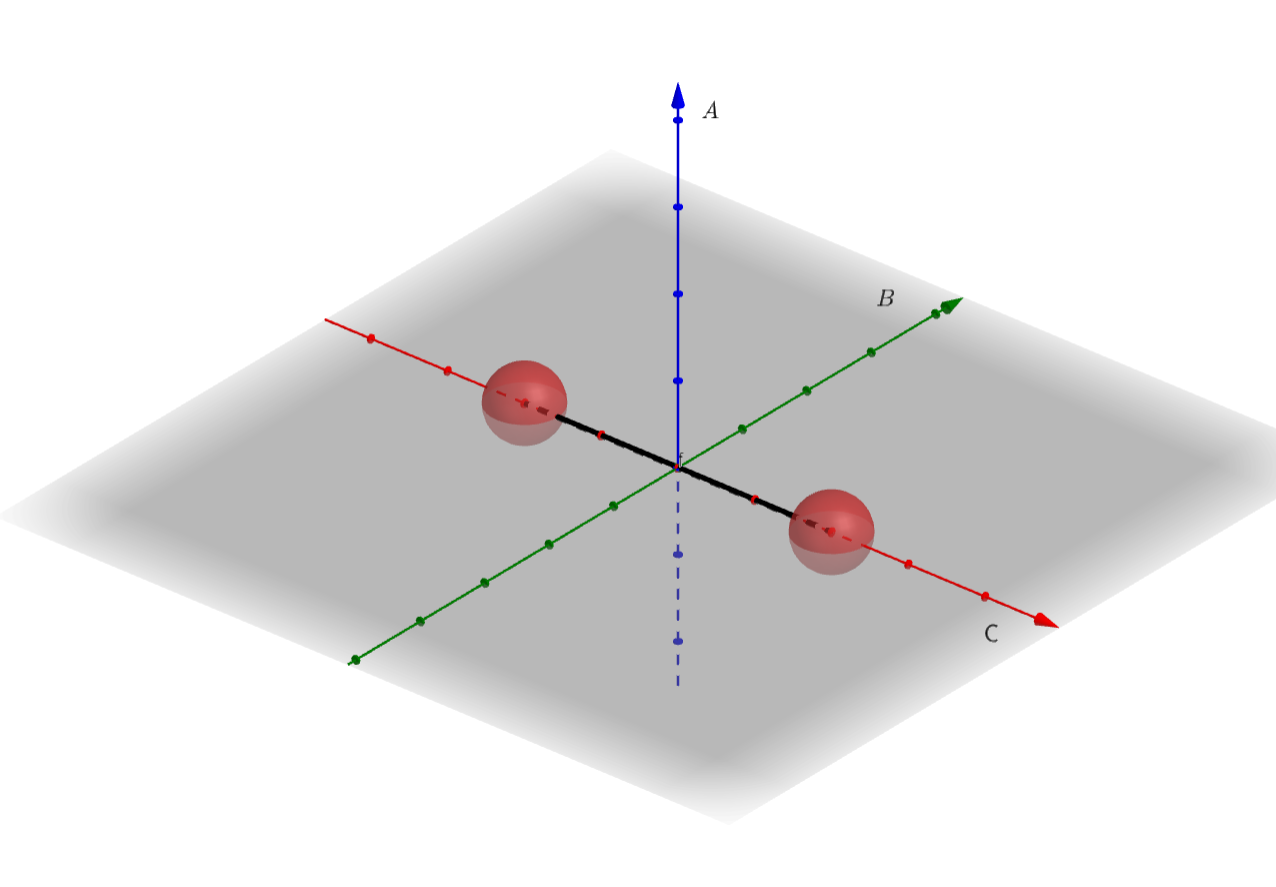
\includegraphics[width=0.6\linewidth]{../images/modello_biatomico1}
	\caption{Schema del modello biatomico con gli assi disposti in modo che il tensore d'inerzia sia diagonalizzato. Uno dei tre assi giace sulla retta congiungente dei due nuclei.}
	\label{fig:modellobiatomico1}
\end{figure}
\FloatBarrier
Notiamo che i due assi perpendicolari alla congiungente dei nuclei non differiscono in nulla dunque avranno la stessa espressione, ricavabile dalla definizione del momento d'inerzia
\begin{align*} 
I_a=I_b=\sum_{i=1}^{2}m_ir_i^2
\end{align*} 
dove \(m_i\) sono le masse degli atomi ed r la distanza tra l'asse e le masse, ovvero metà della distanza (\(d\)) fra i due nuclei. 
\[I_a=I_b=2 m \left(\frac{d}{2}\right)^2 = m\frac{d^2}{2}\]
L'inerzia sull'asse C è diversa perché le sfere ruoteranno ora attorno al loro asse
\begin{align*} 
	I_c = 2 \frac{2}{5}m R^2 
\end{align*} 
dove R è il raggio della sferetta che rappresenta l'atomo, ovvero il raggio atomico.
\begin{figure}[h!]
	\centering
	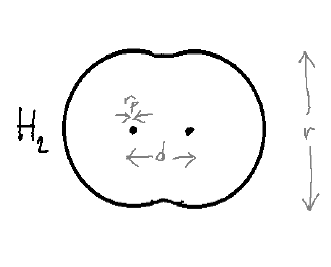
\includegraphics[width=0.4\linewidth]{../images/molecolaH2}
	\caption{Molecola di $H_2$, che esemplifica una semplice molecola biatomica, in cui sono rappresentati R, il raggio della molecola, ed $r_p$, il raggio del protone, che in questo caso coincide con il raggio del nucleo.}
	\label{fig:molecolah2}
\end{figure}
\FloatBarrier
Tuttavia sappiamo che la massa non è equidistribuita nella molecola ma è concentrata nel nucleo dell'atomo che ha raggio dell'ordine di grandezza del raggio del protone ( \(r_p\)), che ha dimensioni trascurabili rispetto a quelle della molecola (che invece compaiono in $I_a$ e $I_b$). La massa degli elettroni, essendo trascurabile rispetto a quella di protoni e neutroni può essere trascurata.
\begin{align*} 
	&d \simeq 0.75\AA = 0.75 \cdot 10^{-10}\ m\\
	&R \simeq 2d\\
	&r_p \simeq 1.7\ fm = 1.7\cdot 10^{-15}\ m\\
	&m_p\simeq_n \simeq 2000m_e
\end{align*} 
Ne deduciamo che l'energia rotazionale rispetto l'asse C è trascurabile dunque
\begin{align*} 
	\varepsilon_{rot} = \frac{1}{2 }I_a \omega_a^2 + \frac{1}{2 } I_b \omega_b^2
\end{align*} 
Ricordando il teorema d'equipartizione dell'energia ne deduciamo che dall'energia rotazionale emergono due gradi di libertà mentre da quella traslazionale 3, i gradi di libertà di un modello siffatto sono 5.\\
Tuttavia, l'approssimazione del legame come un asta rigida non è corretto, questo infatti può vibrare, aggiungendo gradi di libertà al computo totale. Per tenerne conto possiamo modellare il legame come una molla. Scegliamo il nostro sistema di riferimento solidale alla molecola in modo da tenere in considerazione solamente le vibrazioni (le altre energie, già ricavate, restano invariate), in particolare al centro fra le due posizioni di quiete delle molecole. In questa condizione stiamo tenendo conto del movimento elastico di entrambi gli atomi contemporaneamente, per semplificare i calcoli facciamo uso della massa ridotta ($\mu$) in modo da ridurre il modello ad una molla attaccata ad una parete con una massa, fissata ad una estremità della molla, che oscilla. Sia $\xi$ la distanza istantanea della massa dalla posizione d'equilibrio, l'espressione dell'energia sarà la somma di quella cinetica, dovuta alla velocità di vibrazione della massa rispetto al centro di massa, e di quella potenziale, dovuta al potenziale elastico. 
\begin{align*} 
	E = \frac{1}{2}\mu v_{\xi}^2+\frac{1}{2}k\xi^2
\end{align*} 
Per l'equipartizione delle energie abbiamo che un legame aggiunge due gradi di libertà (compaiono due gradi di libertà al quadrato nell'espressione dell'energia). In un sistema siffatto saranno presenti 5+2 = 7 gradi di libertà.\\
Bisogna ora chiedersi: sperimentalmente, quanto ricavato è osservabile? La risposta è negativa: un metodo di verifica è quello di misurare il $c_v$ che dipende direttamente dai d.o.f. Per una molecola monoatomica ci aspetteremmo $c_v = \frac{3}{2} R$ e questo è consistente con le osservazioni, tuttavia quando si osserva una molecola biatomica otteniamo un comportamento del tutto inaspettato: $c_v$ cambia a seconda della temperatura con dei salti che assumono valori, in ordine crescente di temperatura: $\{\frac{3}{2}R\ , \frac{5}{2}R\ ,\frac{7}{2}R\}$. 
\begin{figure}[h!]
	\centering
	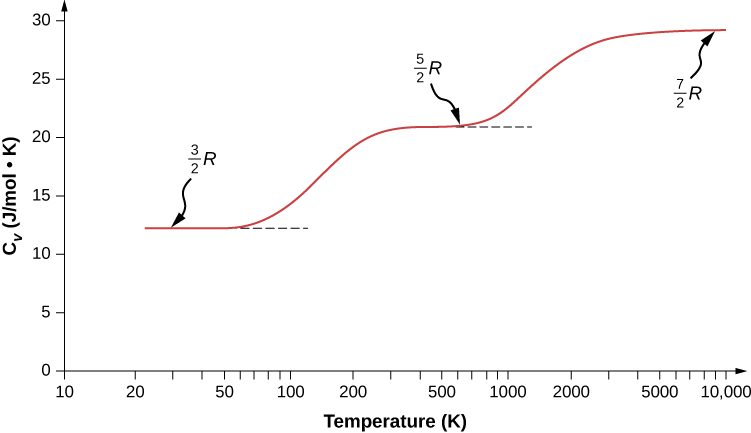
\includegraphics[width=0.6\linewidth]{../images/c_su_T_biatomiche}
	\caption{I vari "salti" di capacità termica in cui si "sbloccano" i d.o.f. di un gas biatomico all'aumentare della temperatura.}
	\label{fig:csutbiatomiche}
\end{figure}
\FloatBarrier
Questo è un limite per la fisica classica con la quale è impossibile spiegare questo comportamento. L'andamento "a gradini", discreto, è invece spiegabile dalla fisica quantistica: esistono delle energie di attivazione caratteristiche in cui si "sbloccano" i vari gradi di libertà. 
\subsection{Molecole poliatomiche}
Cominciamo con il caso con tre atomi, abbiamo due conformazioni possibili: una è quella lineare, come per la $CO_2$ in cui esiste una retta congiungente per i tre nuclei, l'altra è quella angolare, come nel caso dell'$H_2O$ in cui gli atomi si dispongono a triangolo. Come prima, cominciamo approssimando i legami come indeformabili per studiare traslazioni e rotazioni per poi aggiungere le vibrazioni con il modello delle molle.
\begin{figure}
	\centering
	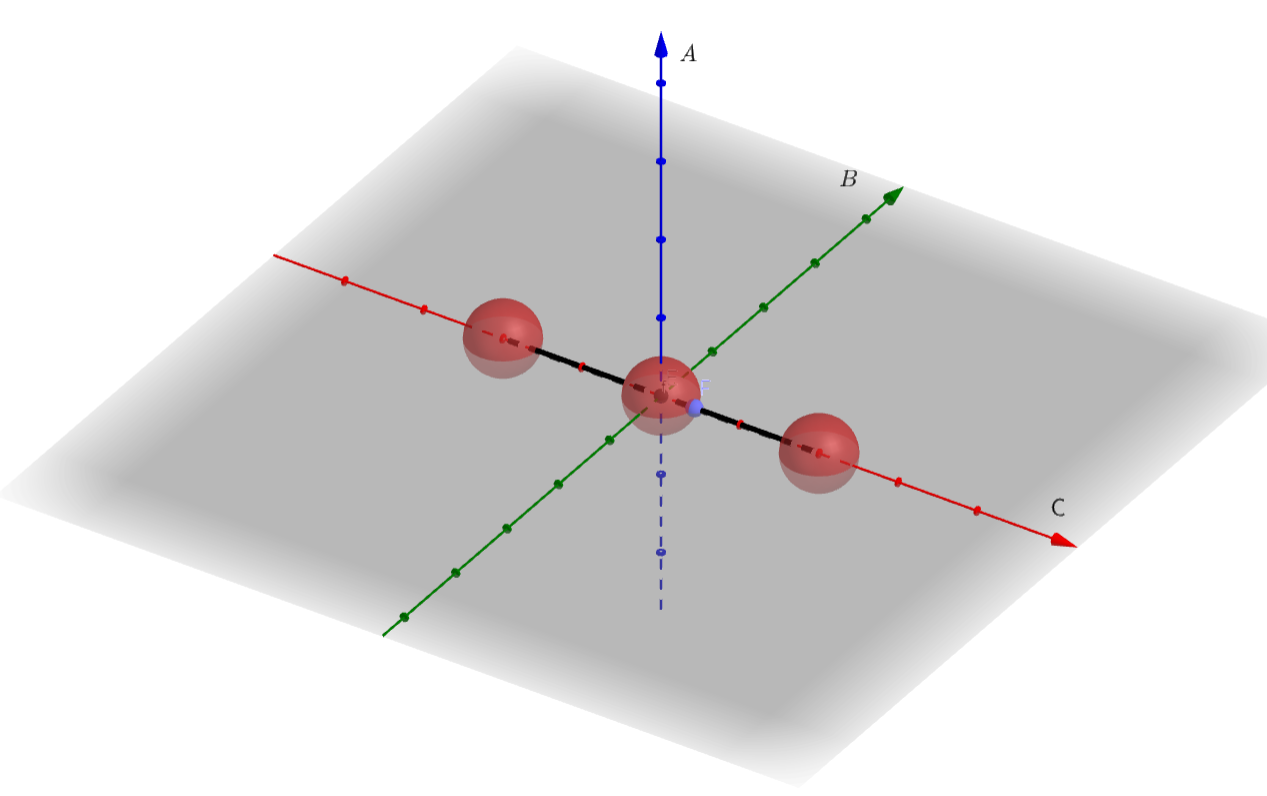
\includegraphics[width=0.4\linewidth]{../images/modello_triatomico1} \quad
	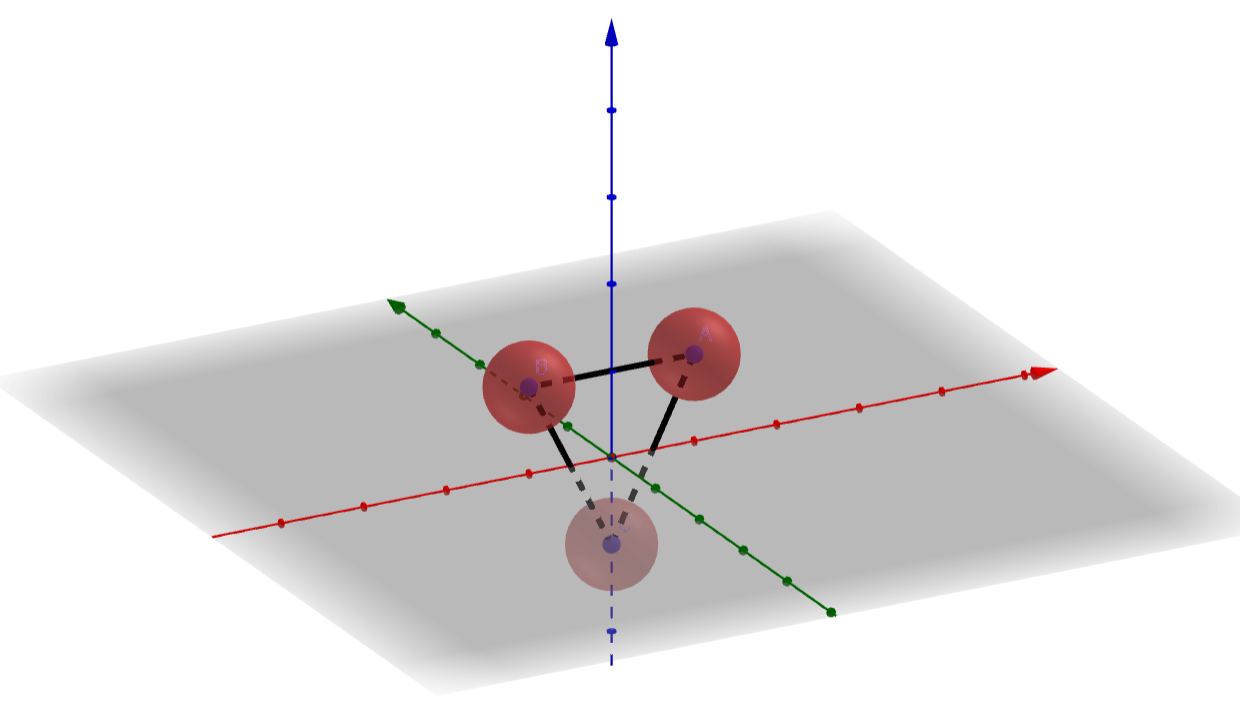
\includegraphics[width=0.4\linewidth]{../images/modello_triatomico2}
	\caption{A sinistra, modello triatomico con forma lineare, a destra con forma angolare. Nel primo caso uno degli assi giace sulla retta passante per i tre nuclei, nel secondo no.}
\end{figure}
\FloatBarrier
Per considerazioni analoghe a quelle per molecole biatomiche, nel caso lineare, a causa della disposizione di un asse in corrispondenza della congiungente, un d.o.f. si semplifica (2 d.o.f dovuti alle rotazioni) mentre nel caso angolare non avviene nessuna semplificazione e si hanno 3 d.o.f. dovuti alle rotazioni.\\
Se al posto dei legami mettiamo delle molle e, come prima scegliamo un S.R.I. solidale al centro della molecola, otteniamo che nel caso lineare esistono 4 modi indipendenti per deformare le molle che tengono unite le molecole mentre in quello angolare 5, ad ognuno di questi modi  si associa un d.o.f. dovuto all'energia cinetica ed uno all'energia potenziale elastica. Avremo così rispettivamente $3+3+5$ gradi di libertà per una molecola triatomica angolare mentre $3+2+4$ per una lineare. Possiamo generalizzare per molecole poliatomiche
\begin{align*}
	&\text{angolare: } \nu = 3+3+2(3N-6)\\
	&\text{lineare: } \nu = 3+2+2(3N-5)\\
	&\Rightarrow c_v^{(lin.)} = \frac{6N-5}{2}R\ ;\quad c_v^{(ang.)}=3(N-1)R	
\end{align*}
\subsection{\(c_p\) e \(c_v\) nei solidi}
\'{E} interessante notare che per un solido, in cui \(c_p\simeq c_v\simeq c\) sono praticamente identici, graficando la variazione di c in funzione della temperatura si ottiene che c cresce fino ad una certa temperatura \(\theta_d\) detta \textbf{temperatura di Debye}, caratteristica per ogni elemento, e poi si stabilizza sempre sul valore di \(3R\). 
\begin{figure}[h!]
	\centering
	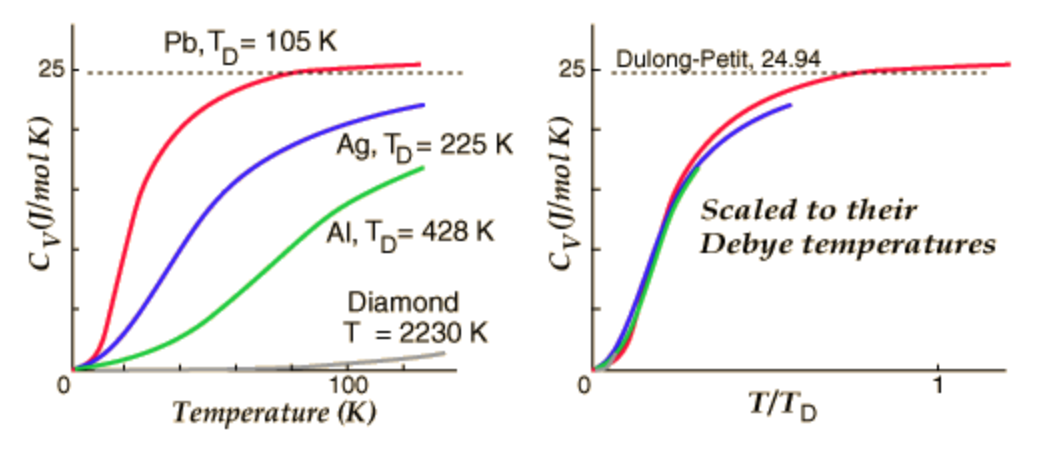
\includegraphics[width=0.7\linewidth]{../images/debye_temperature}
	\caption{A sinistra: grafico capacità su temperatura di diversi elementi. A destra: lo stesso grafico riscalato rispetto alle diverse temperature di Debye.}
	\label{fig:debyetemperature}
\end{figure}
\FloatBarrier
Si è notato sperimentalmente che in un intorno di zero si ha \[c \sim \left(\frac{\theta}{\theta_d}\right)^3\]
Nell'ambito della fisica classica non si riesce a spiegare perché c diminuisca dopo una temperatura di soglia e perché lo faccia quadraticamente; questo fu un grande limite della fisica classica che venne poi risolto dalla fisica quantistica. Tuttavia possiamo spiegarci la stabilizzazione $3R$. In un solido le molecole sono bloccati bloccate e l'unico grado di libertà è quello di vibrazione. Ci sono dunque due componenti indipendenti per ogni direzione (uno di energia cinetica e uno potenziale elastica), risultano così 6 gradi di libertà.
 \[\Rightarrow c = \frac{6}{2}R = 3R\] 
Che è proprio il valore a cui si stabilizza c sperimentale. 
\subsection{Legame tra $c_p$ e $c_v$ in un gas perfetto}
Cominciamo con il trovare \(dQ\) alla luce di quanto visto
\begin{align*}
	&pV = n R \theta \Rightarrow pdV = nRd\theta - Vdp \\
	&dQ = dU+pdV = dU + nRd\theta - Vdp \\
	&n c_vd\theta +nRd\theta - Vdp = n(c_v+R)d\theta-Vdp
\end{align*}
Dove il secondo passaggio è il primo principio della termodinamica a cui è stato sostituito il primo passaggio; nell'ultimo passaggio è stato sostituito quanto trovato nella (\ref{eq:U_gas_perfetti}). Se imponiamo la pressione costante (dp = 0) otteniamo
\begin{align*}
	&(dQ)_p=n(c_v+R)d\theta\\
	&\left(\frac{dQ}{d\theta}\right)_p = n(c_v+R)
\end{align*}
Ricordando la definizione di \(C_p,\ c_p\) e \(c_v\) troviamo un'interessante relazione tra $c_p$ e $c_v$
\begin{align}\label{eq:relazione_di_Mayer}
	&C_p \equiv \left(\frac{dQ}{d\theta}\right)_p = n(c_v+R)\nonumber\\
	&c_p = \frac{1}{n} C_p = (c_v + R)\nonumber\\
	& \Rightarrow c_p - c_v = R
\end{align}
Questa è detta \textbf{Relazione di Mayer}. Sfruttandola, e avendo ricavato i valori di $c_v$ per gas mono, bi e poliatomici possiamo ricavare anche \(c_p \) e\(\gamma\)
\begin{align*}
	&c_p^{(mono)} = \frac{3}{2}R + R = \frac{5}{2}R\\
	&c_p^{(bi)} = \frac{5}{2}R + R = \frac{7}{2} R\\
	&c_p^{(poli,\ ang)} = 3(N-1)R + R = (3N - 2) R\\
	&c_p^{(poli,\ lin)} =  \frac{6N-5}{2}R + R = \frac{6N-3}{2}R\\
	&\gamma^{(ang)} = 1 + \frac{2}{6 N - 6}\\
	&\gamma^{(lin)} = 1 + \frac{2}{6 N - 5}
\end{align*}
Questo modello è valido per N piccoli ma per N che tende a infinito da queste equazioni risulterebbe che gamma in entrambi i casi tende ad 1, sperimentalmente si rileva che gamma tende a $\frac{4}{3}$.
\section{Trasformazioni adiabatiche}
A partire da $\delta Q$ ricavato, consideriamo una trasformazione adiabatica in cui non vi sono scambi di calore. 
\begin{align*}
	&\delta Q = n c_v d\theta + pdV = n c_p d\theta - Vdp = 0\\
	&\begin{cases}
		n c_v d\theta = -pdV\\
		n c_p d\theta = V dp
	\end{cases} \Rightarrow \gamma = - \frac{V}{p}\frac{dp}{dV}\\
	& \frac{dp}{p} = -\gamma \frac{dV}{V} \\
	&\Rightarrow \int\frac{dp}{p} = -\int\gamma \frac{dV}{V}\\
	&\ln(p) = -\gamma \ln(V + cost. = -\ln(V^{\gamma}) + cost.\\
	&\ln(p)+\ln(V^{\gamma}) = cost.\\
	&\ln(pV^{\gamma}) = cost.\\
\end{align*}
\begin{align}\label{eq:adiabatica1}
	&\Rightarrow pV^{\gamma} = cost.
\end{align}
Quest'ultima è una relazione sempre valida per le trasformazioni adiabatiche, da ciò ricaviamo che in un piano di Clapeyron una curva adiabatica è più piccata di una isoterma avendo quest'ultima il volume elevato a potenza ( \(\gamma > 1\)).\\
A partire da questa relazione (in cui compaiono p e V) possiamo ricavarne altre in cui appaiono \(\theta\) e V o \(\theta\) e p. Nel primo caso sostituiamo p, mediante l'equazione di stato dei gas perfetti
\begin{align}\label{eq:adiabatica2}
	&\left(\frac{n R \theta}{V}\right)V^{\gamma} = cost.\nonumber\\
	&n R \theta V^{\gamma - 1} = cost \Rightarrow \theta V ^{\gamma-1}= cost.
\end{align}
Nel secondo caso, sostituiamo V con l'equazione di stato dei gas perfetti in quest'ultima relazione ricavata
\begin{align}\label{eq:adiabatica3}
	&\theta \left(\frac{n R \theta}{p} \right)^{\gamma-1}= \theta (n R \theta^{\gamma-1}) p^{1-\gamma}= cost.\nonumber\\
	&\theta^{\gamma} p^{1-\gamma}= cost.\nonumber\\
	&\theta p^{\frac{1-\gamma}{\gamma}} = cost.
\end{align}
\begin{figure}[h!]
	\centering
	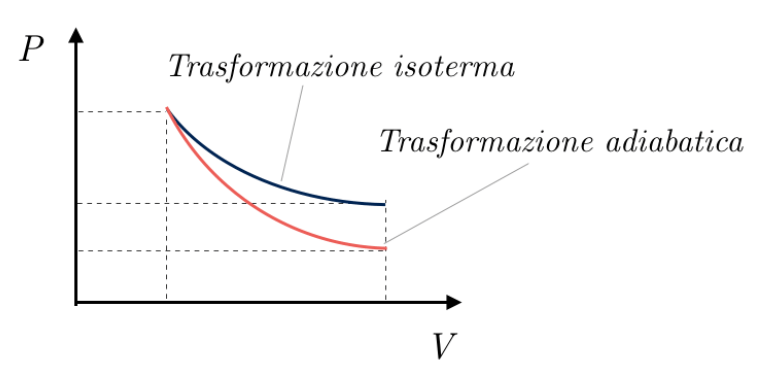
\includegraphics[width=0.6\linewidth]{../images/adiabatica_grafico}
	\caption{Grafico esemplificativo di un'adiabatica ed una isoterma, la prima decresce più rapidamente.}
	\label{fig:adiabaticagrafico}
\end{figure}
\FloatBarrier
\'{E} immediato giustificare la pendenza maggiore della curva adiabatica con la seguente osservazione:
\begin{align*}
	\left(\frac{\partial p}{\partial V}\right)_{isoterma} = -\frac{p}{V} > -\gamma \frac{p}{V} = \left(\frac{\partial p}{\partial V}\right)_{adiabatica}
\end{align*}
\subsection{Calcolo del lavoro di una trasformazione adiabatica}
Come visto per le isoterme, l'area sotto al grafico della trasformazione sul piano di Clapeyron è il lavoro. 
\begin{align*}
	L = \int_{i}^{f} p dV = cost. \int_{i}^{f} V^{-\gamma} dV = \frac{cost.}{1 - \gamma}[V_f^{1-\gamma}-V_i^{1-\gamma}]
\end{align*}
Dove è stata usata la relazione (\ref{eq:adiabatica1}) per sostituire p nell'integrale.\\
Possiamo riscrivere queste relazioni notando che, a partire dalla (\ref{eq:adiabatica1}) otteniamo
\begin{align*}
	&V^{1- \gamma} cost. = pV^{\gamma} V^{1- \gamma} = pV\\
	&\Rightarrow L =  \frac{cost.}{1 - \gamma}[p_f V_f-p_i V_i] = \frac{n R}{\gamma - 1}[\theta_i - \theta_f]
\end{align*}
In quest'ultimo passaggio abbiamo semplicemente usato l'equazione di stato dei gas perfetti e cambiato segno ($\gamma > 1$). Possiamo ora sostituire $\gamma \equiv \frac{c_p}{c_v}$ 
\begin{align*}
L = \frac{n R c_v}{c_p - c_v} [\theta_i - \theta_f] = \frac{n R c_v}{R} [\theta_i - \theta_f] = -n c_v \Delta \theta = -\Delta U
\end{align*}
in quest'ultimo passaggio si ricordi la (\ref{eq:U_gas_perfetti}).\\
Dall'espressione del lavoro possiamo trarre alcune conclusioni: se L > 0 si ha un'espansione adiabatica e il gas si raffredda: \(\Delta \theta< 0\), se L < 0 si ha una compressione adiabatica e il gas si riscalda : \(\Delta \theta > 0\), se L = 0 si ha un'espansione libera in cui, come visto nell'esperimento di Joule \(\theta_f = \theta_i\).
\begin{exercise}[Espansione adiabatica]
	Mostrare, usando il modello della T.C.G., che durante un’espansione adiabatica quasistatica
	un gas si raffredda.\\
	Consideriamo il gas nel cilindro+pistone, e concentriamoci su una singola molecola di cui andremo	a considerare la componente della velocità parallela al movimento del pistone (le altre componenti non cambiano modulo, essendo gli urti elastici). Sia v la velocità della molecola (verso l’alto) e V < v la velocità del pistone (sempre verso l’alto poiché è un'espansione). Mettiamo a sistema conservazione dell'energia e della quantità di moto
	\begin{align*}
		\begin{cases}
			\frac{1}{2} m v^2 + \frac{1}{2}M V^2 = \frac{1}{2}M V'^2+\frac{1}{2}m v'^2\\
			m v + M V = m v' + M V'
		\end{cases} \Rightarrow 
		\begin{cases}
			v' = \frac{(m - M) v + 2 M V}{m + M}\\
			V' = \frac{(M - m)V + 2m V}{m + M}
		\end{cases}
	\end{align*}
Se il rapporto \(r \equiv \frac{m}{M}\) tende a 0 (poiché la massa della molecola è molto inferiore di quella del pistone siamo nelle condizioni di una pallina che colpisce un muro elasticamente) avremmo
\begin{align*}
	\begin{cases}
		v' = -v + 2 V\\
		V' = V
	\end{cases}
\end{align*}
Possiamo quindi calcolare la variazione di energia cinetica della molecola, che corrisponde alla variazione di temperatura del gas dovuta all'urto di una singola molecola (ma le altre molecole si comporteranno analogamente dunque studiando l'energia cinetica di una molecola possiamo avere informazioni sulla temperatura). 
\begin{align*}
	\Delta\varepsilon = \varepsilon' - \varepsilon = \frac{1}{2} m (v'^2 - v^2) = \frac{1}{2} m [(-v+2v)^2 - v^2] = 2 m V (V - v)
\end{align*}
Ne deduciamo che 
\begin{itemize}
	\item se V > 0 (espansione) e V< v allora $\Delta\varepsilon < 0$ dunque si ha un raffreddamento
	\item se V < 0 (compressione) e V< v allora $\Delta\varepsilon > 0$ dunque si ha un riscaldamento
	\item se $V\to\infty$ la molecola non urta, saremmo dunque nel caso di un'espansione libera in cui  $\Delta\varepsilon = \Delta \theta = 0$
\end{itemize}
\end{exercise}
\subsection{Applicazioni delle espansioni adiabatiche}
\subsubsection{Espansione dell'universo}
A seguito di conferme sperimentali si è arrivati alla conclusione che l'universo è in espansione, è interessante studiarne gli effetti mediante le conoscenze di termodinamica classica acquisite. Gli assunti che stanno alla base di questa trattazione sono che l'universo sia omogeneo ed isotropo e che sia modellizzabile come un fluido composito (stelle, pianeti ecc.) ma principalmente formato da fotoni liberi (fotoni primordiali). Inoltre sembra ovvio assumere che l'espansione dell'universo è libera visto che si sta espandendo nel vuoto (cosa ci sarebbe al di là dell'universo se no?).\\
Isoliamo una regione sferica di volume V e con energia interna U di universo, definiamo il rapporto \(\rho = \frac{U}{V}\) e calcoliamone il differenziale. 
\begin{align*}
	d\rho = d\left(\frac{U}{V}\right) = \frac{d U}{V}- U \frac{dV}{V^2} = \frac{dU}{V}-\rho\frac{dV}{V}
\end{align*}
Essendo l'espansione adiabatica si ha \(dU = -pdV)\) e quindi, sostituendo
\begin{align*}
	d\rho = -\frac{pdV}{V}- U \frac{dV}{V^2} = \frac{dU}{V}-\rho\frac{dV}{V} = -(p + \rho)\frac{dV}{V}
\end{align*}
Dobbiamo però fare una breve digressione per chiarire come l'universo si espanda: in realtà, a differenza dell'espansione di un gas, in questo caso è lo spazio stesso ad espandersi, trascinando con sè tutto ciò che vi si trova dentro (per la relatività generale lo spazio è un mezzo elastico deformabile), l'espansione avviene indipendentemente da ciò che c'è dentro lo spazio. Per esprimere questa espansione si usa un fattore di scala $a(t)$ che stabilisce come cambia la distanza fra due punti nel tempo, se a $t_0$ questi avevano distanza $d_0$, dopo un intervallo di tempo si avrà \(d(t) = a(t)\cdot d_0\).\\
Da questa informazione possiamo sapere come si espande la regione sferica tenuta in considerazione in funzione del tempo: sia $r_0$ il raggio iniziale della sfera e $V_0 \equiv \frac{4}{3}\pi r_0^3$il volume iniziale
\begin{align*}
	&V(t) = \frac{4}{3}\pi[a(t) r_0]^3 = \frac{4}{3}\pi a(t)^3 r_0^3\\
	&dV = (3 a^2 da) V_0\\
	&\frac{dV}{V} = \frac{(3 a^2 da) V_0}{\frac{4}{3}\pi a(t)^3 r_0^3} = \frac{(3 a^2 da) V_0}{ a(t)^3 r_0^2} =\frac{3 da}{a}
\end{align*}
Ricordando il valore di $d\rho$ ottenuto precedentemente possiamo dividere ambo i membri per dt e trovare una relazione fra derivate
\begin{align*}
	&\frac{d\rho}{dt} = -3(p + \rho)\frac{1}{a}\frac{da}{dt}\\\
	&\dot{\rho} = -3(p + \rho)\frac{\dot{a}}{a}
\end{align*}
Notiamo che la variazione della densità di energia interna varia come la variazione del "rate" d'espansione fratto il rate d'espansione stesso, questo rapporto è stato dimostrato essere costante ed è detto \textbf{costante di Hubble} indicata come \(\frac{\dot{a}}{a}\equiv H\).  Possiamo così riscrivere l'equazione precedente
\[\dot{\rho} = -3(p+\rho) H\]
Quest'ultima è nota come una delle equazioni di Aleksandr Friedmann (1888 - 1925), ottenute da alcune delle soluzioni delle equazioni della relatività generale. Visto che abbiamo trovato questa equazione assumendo l'universo in espansione adiabatica, e dalla relatività generale si perviene allo stesso risultato, possiamo affermare che la R.G. prevede un universo in espansione adiabatica. 
\begin{figure}[h!]
	\centering
	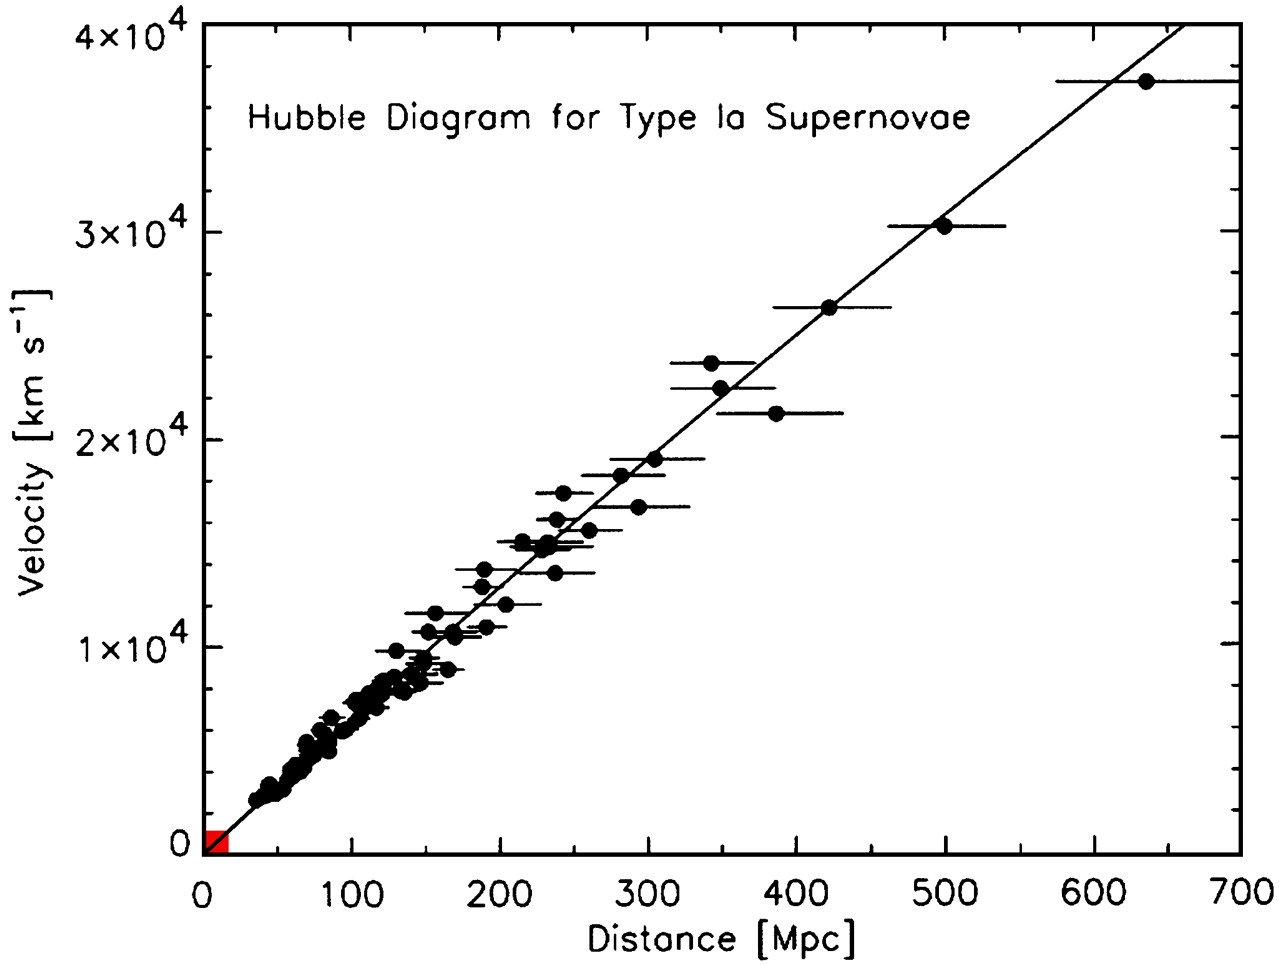
\includegraphics[width=0.6\linewidth]{../images/Hubble}
	\caption{Grafico velocità di espansione su espansione in cui ogni punto indica una galassia a diversa distanza; i dati sperimentali confermano la legge di Hubble.}
	\label{fig:hubble}
\end{figure}
\FloatBarrier
Volgiamo ora ricavare come varia la temperatura dell'universo in funzione del tempo, questo può fornirci un'enorme quantità di informazioni utili su di esso.\\
Per far ciò serve conoscere l'equazione di stato del fluido \(p(\rho)\), da cui sono ricavabili sia la funzione \(a(t)\) che $\gamma$. Si è arrivato a sapere che per un fluido di tipo "radiazione" come il gas di fotoni, si ha \[a(t)\propto t^{\frac{1}{2}}\ , \gamma = \frac{4}{3}\] mentre per uno di tipo "materia" come per i barioni, si ha \[a(t)\propto t^{\frac{2}{3}}\ , \frac{5}{3}\]. Data la relazione (\ref{eq:adiabatica2}) per le trasformazioni adiabatiche quasistatiche e con gas perfetti (cosa che sono gas di fotoni e barioni), e ricordando che \(V(t)\) varia come \(a(t)^3\), otteniamo
\begin{itemize}
	\item Radiazione: \(\theta V^{1-\gamma} = \theta V^{\frac{1}{3}} \Rightarrow \theta a = cost.\)
	\item Materia: \(\theta V^{1-\gamma} = \theta V^{\frac{2}{3}} \Rightarrow \theta a^2 = cost.\)
\end{itemize}
Avendo ipotizzato inizialmente  che la nostra porzione di universo è permeata da gas di fotoni, concentriamoci sulla relazione valida per le radiazioni, abbiamo una proporzionalità inversa dunque
\begin{align*}
	&a = \frac{cost.}{\theta} \Rightarrow  \theta t^{\frac{1}{2}} = cost.
\end{align*}
Portiamo ora questa relazione in scala logaritmica
\[\ln(\theta) = -\frac{1}{2}\ln(t) + cost.\]
Ecco ottenuta la relazione che cercavamo. Sapendo approssimativamente la vita dell'universo, e quindi i secondi che ci separano dal big bang ( circa $4\cdot 10^{17}\ s$), e conoscendo la temperatura dell'universo attuale (pari a circa 3\textdegree k) possiamo ricavare la temperatura dell'universo in qualunque tempo cosmologico. 
\begin{align*}
	&\ln(3) = -\frac{1}{2}\ln(4\cdot10^17) + cost.\\
	& cost. = \ln(3) + \frac{1}{2}\ln(4\cdot10^{17}) \simeq 21\\
	&\Rightarrow \ln(\theta) = -\frac{1}{2}\ln(t) + 21
\end{align*}
\'{E} interessante sapere che l'energia (e quindi temperatura) massima raggiunta in laboratorio sulla terra è quella del collisore LHC del CERN di Ginevra che corrisponde a $13 TeV = 1.3 \cdot 10^{13} eV = 1.3 \cdot 10^{13} \cdot 1.16 \cdot 10^4\ °K = 1.5\cdot 10^{17}\ °K $. Possiamo ricavare a quale tempo cosmico corrisponde questa temperatura
\begin{align*}
	& \ln(t) = 2(21 -\ln(\theta)) \simeq -36 \\
	& t \simeq e^{-36} \simeq 10^{16}
\end{align*}
\begin{figure}[h!]
	\centering
	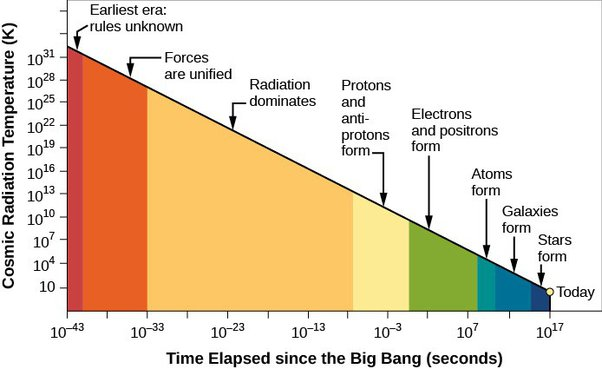
\includegraphics[width=0.6\linewidth]{../images/temperatura_universo}
	\caption{Grafico in scala doppio logaritmica della temperatura dell'universo in funzione del tempo cosmico. Si noti che c'è una soglia di tempo, detta \textbf{tempo di Planck} oltre il quale le leggi della fisica non valgono e le leggi della fisica quantistica e relativistica si contraddicono. Ciò, insieme ad altre considerazioni, ci suggerisce che le teorie odierne sono incomplete.}
	\label{fig:temperaturauniverso}
\end{figure}
\FloatBarrier
Infine, si può osservare come un universo in espansione conduce a un lento e progressivo
raffreddamento verso lo zero assoluto, scenario che in ambito cosmologico va sotto il nome
di\textbf{ morte fredda dell’Universo}.
\subsubsection{Dipendenza della temperatura dalla quota}
Nell'esercizio (\ref{ex:pressione_quota}) abbiamo ricavato una relazione che connette la pressione atmosferica con la quota, abbiamo tuttavia ipotizzato la temperatura costante al variare della quota, approssimazione che ci faceva sottostimare il valore misurato della pressione. Ci proponiamo ora di studiare la variazione di temperatura in funzione della quota per poi correggere la relazione trovata in precedenza. Partiamo da quanto già ricavato (\ref{eq:esercizio_pressione})
\[\frac{dp}{p} = \frac{M g(z)}{R\theta(z)} dz\]
Innanzitutto, bisogna svolgere una breve digressione su cosa accada quando l'aria viene riscaldata in atmosfera. I fotoni provenienti dal sole aumentano la temperatura dell'aria che, espandendosi, diminuisce la sua densità. Per la legge di Archimede, questa massa d'aria sale ma salendo di quota incontra strati d'atmosfera a pressione inferiore, avviene così un'altra espansione di tipo adiabatico (tutte le trasformazioni dell'aria sono considerate adiabatiche data la sua scarsissima capacità termica). Usiamo la (\ref{eq:adiabatica3}) facendone il logaritmo e calcolandone il differenziale. 
\begin{align*}
	&\theta p^{\frac{1-\gamma}{\gamma}} = cost\\
	&\ln(\theta p) + \frac{1-\gamma}{\gamma}\ln(p) = cost.\\
	&\frac{d\theta}{\theta}+\frac{1-\gamma}{\gamma}\frac{dp}{p} = 0\\
	&\frac{dp}{p} = -\frac{\gamma}{1-\gamma}\frac{d\theta}{\theta}
\end{align*}
Possiamo eguagliare quest'ultima con l'espressione di $\frac{dp}{p}$ ottenuta nell'esercizio già fatto
\begin{align*}
	&-\frac{\gamma}{1-\gamma}\frac{d\theta}{\theta} = \frac{M g}{R \theta}dz\\
	&\frac{d\theta}{dz} = -\frac{\gamma - 1}{\gamma} \frac{M g}{R}
\end{align*}
Definiamo ora il gradiente termico L come
\begin{align*}
	&L \equiv \frac{\gamma - 1}{\gamma} \frac{M g}{R}\\
	&\frac{d\theta}{dz} = -L 
\end{align*}
Il segno negativo indica che all'aumentare della quota la temperatura diminuisce.\\
Ad esempio, possiamo valutare L dell'aria considerandola un gas biatomico perfetto
\[\gamma = \frac{7}{5},\ M = 28.8\ g,\ \Rightarrow L \simeq 9.7\cdot 10^3\ \frac{K}{m} \simeq 10\ \frac{K}{km}\]
Tuttavia, questa previsione classica sovrastima ancora il valore misurato poiché non tiene conto della condensa dell'aria: il calore latente di condensa trattiene calore e diminuisce la temperatura. Il vero gradiente termico è $6.5\ \frac{K}{km}$. Possiamo dunque determinare la temperatura in funzione della quota, conoscendo la temperatura alò livello del mare $\theta_0$ integrando 
\begin{align*}
	&\int d\theta = -\int L dz\\
	&\theta (z) = \theta_0 - L z
\end{align*}
Questo approccio però ha validità solamente nei primi 10 km inferiori dell'atmosfera poiché a questa quota avvengono fenomeni che portano ad un'inversione di tendenza (come la formazione di ozono). 
\begin{figure}[h!]
	\centering
	\includegraphics[width=0.6\linewidth]{"../images/temperatura atmosferica"}
	\caption{Grafico della temperatura in funzione della quota. La nostra trattazione è valida solamente nella troposfera. Si notino le varie inversioni di tendenza.}
	\label{fig:temperatura-atmosferica}
\end{figure}
\FloatBarrier
\section{Metodi per il calcolo di $\gamma$}
\subsection{Esperimento di Ruchardt}
In questo esperimento la misura di \(\gamma\) avviene tramite la misura del periodo d'oscillazione di una pallina posto all'imboccatura di un recipiente di vetro di volume V.
\begin{figure}[h!]
	\centering
	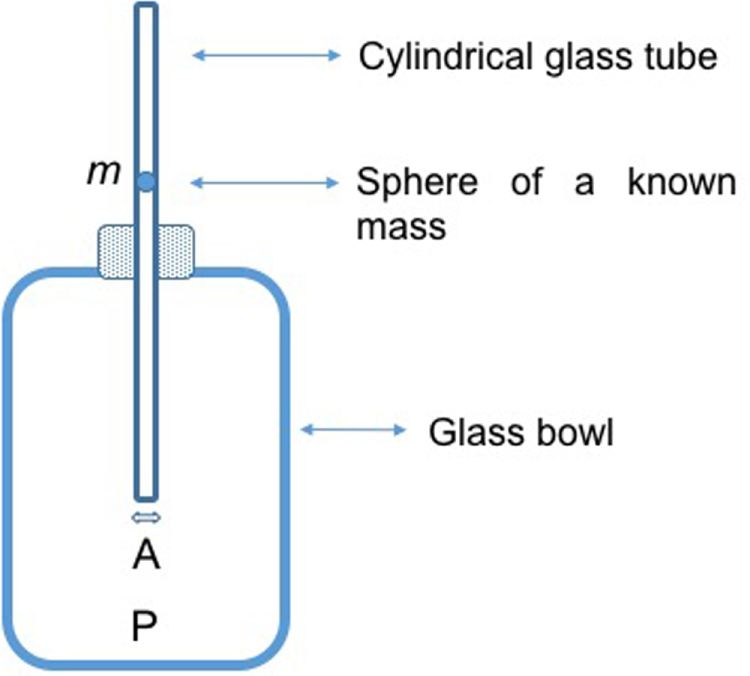
\includegraphics[width=0.4\linewidth]{../images/ruchardt}
	\caption{Schema dell'apparato sperimentale di Ruchardt.}
	\label{fig:ruchardt}
\end{figure}
\FloatBarrier
 All'equilibrio la pressione interna eguaglia quella atmosferica più quella esercitata dalla pallina. \[p = p_0 + \frac{m g}{A}\] Dove A è la superficie dell'imboccatura. Se si perturba l'equilibrio con una forza \(dF = A dp\) la pallina comincerà a muoversi modificando il volume e quindi la pressione e temperatura all'interno del recipiente. Vista la velocità delle trasformazioni possiamo considerarle le adiabatiche, vale dunque la relazione \(\frac{dp}{p}=-\gamma\frac{dV}{V}\), sostituendo
 \begin{align*}
 	&dp = -\gamma p \frac{dV}{V}\\
 	&dF = A dp = - A \gamma p \frac{dV}{V} = - \frac{A^2 \gamma p}{V}dz
 \end{align*} 
 Dove nell'ultimo passaggio si è sostituito $dV = A dz$. Notiamo che integrando la precedente, per il secondo principio della dinamica otteniamo l'equazione tipica dell'oscillatore armonico. 
 \begin{align*}
 	&\int dF = -\int  \frac{A^2 \gamma p}{V}dz\\
 	&F = m \ddot{z}= - \frac{A^2 \gamma p}{V} z\\
 	&\ddot{z} + \frac{A^2 \gamma p}{m V} z = 0 \Rightarrow \tau = 2\pi \sqrt{\frac{mV}{\gamma p A^2}}\\
 	&\gamma = \frac{4 \pi^2 m V}{A^2 p \tau^2}
 \end{align*}
Abbiamo così ottenuto una relazione in cui gamma è misurabile. La precisione della misura su $\tau$, essendo elevato al quadrato, ha molta influenza sull'incertezza di $\gamma$. 
\subsection{Velocità del suono}
Un metodo più preciso consiste nel misurare la velocità di propagazione delle onde sonore
in un gas per inferire il valore di $\gamma$. In generale la velocità di propagazione delle onde sonore è data dalla relazione
\begin{align*}
	v = \sqrt{\frac{k_s}{\rho}}
\end{align*}
Dove $\rho$ è la densità del mezzo e $k_s$ il \textbf{modulo di comprimibilità adiabatico} che è definito come \[\frac{1}{k_s}\equiv -\frac{1}{V}\left(\frac{\partial V}{\partial p}\right)_s\]
Dove la s sta ad indicare che non vi sono scambi di calore.\\ In un gas la propagazione di un'onda sonora può essere vista come una compressione o espansione del mezzo che avviene adiabaticamente essendo estremamente rapida. Possiamo dunque scrivere
\begin{align*}
	&\frac{dp}{p} = -\gamma \frac{dV}{V}\\
	&-\frac{1}{V}\frac{dV}{dp}=\frac{1}{\gamma p} = \frac{1}{k_s}\\
	&k_s = \gamma p \Rightarrow v = \sqrt{\frac{\gamma p}{\rho}}
\end{align*}
Da questa relazione possiamo ricavare l'espressione di $\gamma$ in cui compaiono solo grandezze misurabili \[\gamma =\frac{ \rho v^2}{p}\]
\begin{exercise}[Calcolo della capacità termica]
Sia la capacità termica di un gas perfetto monoatomico nella trasformazione $\tau$ \[C = \frac{1}{n}\left(\frac{\delta Q}{d\theta}\right)_{\tau}\] 
Dove $\tau$ è la trasformazione che porta dallo stato A: ($p_0$, $V_0$) a quello B:($p_0/2$, $2V_0$) come riportato in figura
\begin{figure}[h!]
	\centering
	\includegraphics[width=0.5\linewidth]{../images/esercizio_capacità}
	\caption{Grafico della trasformazione $\tau$}
	\label{fig:eserciziocapacita}
\end{figure}
\FloatBarrier
Si calcoli la funzione della capacità termica in funzione del volume \(C_{\tau}(V)\).\\\\

La strategia di risoluzione (valida in generale per questo tipo di problemi) è quella di trovare una espressione di $\delta Q$ in cui si possa mettere in evidenza \(d\theta\) per poi trovare il rapporto \(\left(\frac{\delta Q}{d\theta}\right)_{\tau}\). Cominciamo con lo scrivere il primo principio 
\begin{align*}
	\delta Q = dU + pdV = n c_v d\theta + pdV = \left(n \frac{3}{2} R\right) d\theta + pdV
\end{align*} 
dove è stato sostituito $c_v$ considerando l'ipotesi di gas monoatomico perfetto. Si noti che se il secondo termine della somma non ci fosse avremmo già risolto il problema perché avremmo trovato un'espressione di $\delta Q$ in funzione di $d\theta$; questo sarebbe il caso in cui la trasformazione fosse a volume costante. Volendo mantenere la generalità, cerchiamo di esprimere sia $p$ che $dV$ in funzione di $d\theta$. Ricavare \(p(V)\) è semplice considerando che la funzione che descrive la trasformazione è quella di una retta. Scriviamo la funzione di una retta passante per i due punti A e B di coordinate \((p_0, V_0)\) e \((\frac{p_0}{2}, 2 V_0)\)
\begin{align*}
	&p-p_0 = \frac{\frac{p_0}{2}-p_0}{2V_0 - V_0}(V-V_0) = -\frac{p_0}{2V_0}(V-V_0) \\
	&\Rightarrow p = p_0 \left(\frac{3}{2} - \frac{V}{2 V_0}\right)
\end{align*}  
Per ricavare dV in funzione di $d\theta$ usiamo l'ipotesi per cui il gas è perfetto. Dall'equazione di stato dei gas perfetti, sostituiamo p con la relazione appena ricavata
\[\left[p_0\left(\frac{3}{2} - \frac{V}{2 V_0} \right) \right] V = n R \theta \] 
Possiamo quindi differenziare quest'ultima equazione ed isolare $dV$
\begin{align*}
	&p_0\left(\frac{3}{2}dV - \frac{V}{V_0}dV\right) = n r d\theta\\
	&\Rightarrow dV = \left[\frac{n R}{p_0 \left(\frac{3}{2}-\frac{V}{V_0}\right)}\right]d\theta
\end{align*}
Possiamo infine sostituire quanto trovato nell'espressione di $\delta Q$ per poi sostituire \(x \equiv \frac{V}{V_0}\) e svolgere semplificazioni
\begin{align*}
	\delta Q &= \left(n \frac{3}{2} R\right) d\theta + p_0 \left(\frac{3}{2} - \frac{V}{2 V_0}\right) \cdot \left[\frac{n R}{p_0 \left(\frac{3}{2}-\frac{V}{V_0}\right)}\right]d\theta =\\
	&\left(n \frac{3}{2} R\right) d\theta + p_0 \left(\frac{3}{2} - \frac{x}{2}\right) \cdot \left[\frac{n R}{p_0 \left(\frac{3}{2}- x \right)}\right]d\theta= n R \frac{15-8x}{6-4x}d\theta\\
	&\Rightarrow \frac{\delta Q}{d\theta}_{\tau} = n R \frac{15-8x}{6-4x}\\
	&C_{\tau}(x) = \frac{1}{n}\frac{\delta Q}{d\theta}_{\tau} = R \frac{15-8x}{6-4x}
\end{align*}
Il problema è risolto. Risulta però molto interessante svolgere lo studio di funzione di quanto ottenuto il relazione al grafico della trasformazione. \\
Preliminarmente, notiamo che per \(x = 1\) abbiamo \(C_{\tau}(1) = \frac{7}{2}R\). Possiamo studiare il grafico della funzione ponendo sull'asse y \(\frac{C_{tau}}{\frac{7}{2}R}\). Inoltre, visto che il denominatore si annulla per \(x = \frac{3}{2}\), abbiamo che la funzione tende a \(+\infty \) da sinistra e a  \(-\infty\) da destra per il limite di $x \to \frac{3}{2}$; avremo un asintoto verticale. La funzione si annulla per $x = \frac{15}{8}$.

\begin{figure}[h!]
	\centering
	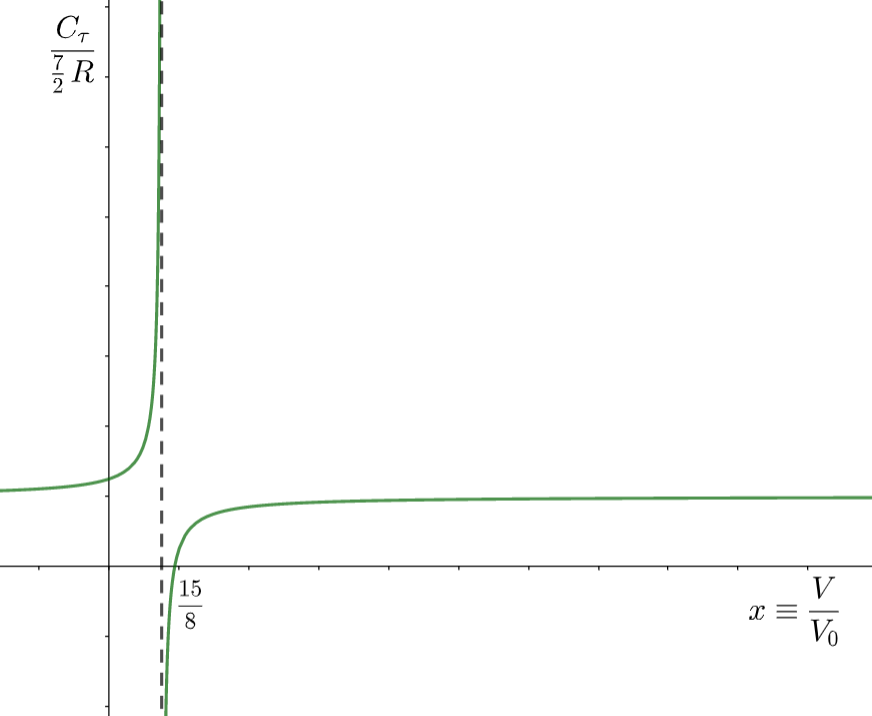
\includegraphics[width=0.45\linewidth]{../images/studio_di_funz}\quad
	\includegraphics[width=0.45\linewidth]{../images/esercizio_capacità2}
	\caption{Grafico della funzione $C_{\tau}(x)$ affiancato da quello della trasformazione sul piano di Clapeyron.}
	\label{fig:studiodifunz}
\end{figure}
\FloatBarrier

Interpretiamo ora il grafico della funzione $C_{\tau}(x)$ in relazione a quello della trasformazione sul piano di Clapeyron.\\

Richiamando il primo principio \[\delta Q = dU + \delta L\] si ha che $\delta L > 0$ sempre, poiché la trasformazione è un'espansione, mentre dU varia allo stesso modo di $\delta\theta$, visto che stiamo considerando un gas perfetto in cui la temperatura coincide con l'energia interna a meno di una costante.
Si consideri inoltre che quando x è nel punto medio fra A e B, ovvero ad \(M=\frac{3}{2}\) si ha l'asintoto; ne segue che in un intorno sinistro di $\frac{3}{2}$, $C_{\tau}$ è positivo mentre in quello destro negativo (in M avviene un cambio di segno). Ora, ricordando che \[C_{\tau}(x) = \frac{1}{n}\left(\frac{\delta Q}{d\theta}\right)_{\tau}\] se questo è maggiore di zero da 1 a $\frac{3}{2}$ si ha che il rapporto è crescente dunque può accadere o \(d\theta > 0\) e \(\delta Q > 0\) oppure \(d\theta < 0\) e \(\delta Q < 0\). Tuttavia, considerando le curve isoterme che intersecano la trasformazione $\tau$ si deduce che il segno di $d\theta$ è positivo fino ad M e negativo da M a B dunque bisognerà accettare l'ipotesi che \(d\theta > 0\) e \(\delta Q > 0\). \\
Per \(x = \frac{3}{2}\), ovvero in M, \(d\theta = 0\) e \(dU = 0\),siamo nelle condizioni di una trasformazione isoterma. Interpretiamo la capacità termica infinita, in un intorno infinitesimo di M, come: "indipendentemente da quanto calore fornisco, la temperatura non cambia".
Per x compreso fra $\frac{3}{2}$ e 2 \(d\theta < 0\) e \(dU < 0\) ma visto che \(\delta Q = dU + \delta L\) nonostante dU sia negativo, a causa della presenza di $\delta L > 0$, esiste una regione in cui $\delta Q$ continua ad essere positivo e dunque la capacità risulta negativa (numeratore positivo e denominatore negativo). Interpretiamo la capacità negativa come: "fornendo energia la temperatura diminuisce". Questa regione va da M ad $N = \frac{15}{8}$ (in cui la capacità termica è nulla).
Nel punto N in cui $C_{\tau}=0$ siamo in condizioni di adiabaticità locale: in un intorno infinitesimo di questo punto non si scambia calore con l'esterno. In corrispondenza di questo punto la curva della trasformazione adiabatica corrispondente è tangente al grafico della trasformazione $\tau$.
Quando la componente in dU (negativa) sovrasta $\delta L$ anche $\delta Q < 0$ dunque la capacità tornerà positiva (sia numeratore che denominatore negativi), ciò corrisponde alla regione da N a B. 
\end{exercise}
\section{Trasmissione del calore}
Come visto, il calore è stato introdotto formalmente a seguito dell'enunciazione del primo principio della termodinamica. La sua funzione è essenzialmente quella di ristabilire la conservazione di energia in presenza di lavoro non-adiabatico (non conservativo). Trasferire calore, in assenza di lavoro termodinamico, ha l'effetto macroscopico di aumentare la temperatura, se ne deduce che il trasferimento di calore è un trasferimento di energia cinetica da un punto ad un altro dello spazio. Studiare il trasferimento di calore vuol dire studiare il passaggio da uno stato di equilibrio ad un altro, siamo interessati quindi ad una trasformazione: compare per questo la variabile tempo, fin ora mai usata (poiché abbiamo studiato solo stati di equilibrio). Esistono 3 distinte modalità di trasferimento di calore, vediamole.
\subsection{Conduzione}\label{sec:conduzione}
Si ha conduzione termica quando il trasferimento di calore avviene senza spostamento macroscopico di materia. Ad esempio, nei solidi lo scambio avviene a causa dell'oscillazione elastica del reticolo o dall'oscillazione degli elettroni nella banda di conduzione. \\
La \textbf{Legge di Fourier} è una legge empirica che descrive il passaggio di calore per conduzione: presa una porzione infinitesima di sostanza di superficie dA e spessore dx, posta fra due temperature $\theta$ e $\theta+d\theta$, la quantità di calore trasferita da una faccia all'altra della sostanza è pari a 
\[\frac{\delta Q}{dt}= - k dA \frac{d\theta}{dx}\]
La variazione del tempo del calore ha come unità il Watt ed è una potenza. Questa legge ci dice che il trasferimento di calore avviene dalla superficie a temperatura maggiore a quella minore (a causa del segno meno) proporzionalmente al gradiente di temperatura (la differenza di temperatura rispetto allo spessore), alla superficie di contatto e di una costante k (di dimensione \(W m^{-1} K^{-1}\)) detta \textbf{conducibilità termica}. Fisicamente, rappresenta un indice di "quanto bene la sostanza conduce il calore";  in generale la conducibilità termica può dipendere dalla temperatura (ad esempio nei gas $k = f(\sqrt{\theta}$)). Ecco alcuni esempi
\begin{itemize}
	\item $k_{Ag} = 400 W m^{-1} K^{-1}$
	\item $k_{ghiaccio} = 2 W m^{-1} K^{-1}$
	\item $k_{vetro} = 1 W m^{-1} K^{-1}$
	\item $k_{aria} = 0.02 W m^{-1} K^{-1}$
\end{itemize} 
Notiamo che i metalli sono ottimi conduttori e che a loro confronto l'aria ha conducibilità termica minore di 4 ordini di grandezza, per questo motivo, molte delle trasformazioni dell'aria possono essere approssimate come adiabatiche (scarso scambio di calore per conduzione). \'{E} possibile applicare la legge di Fourier, con opportuni integrali, a forme diverse di conduttori, di seguito sono riportati alcuni semplici esempi
\begin{exercise}[Conduttore con geometria planare omogeneo posto fra due termostati]
	Si consideri un parallelepipedo di spessore d e con una facce di area A che deve isolare la temperatura interna $\theta_1$ da quella ambientale $\theta_2$. Il flusso di calore è costante dunque lo è anche il gradiente termico. Integrando l'equazione di Fourier per tutto lo spessore d si ottiene 
	\begin{align*}
		&P = \frac{\delta Q}{dt} = \frac{k A (\theta_1 - \theta_2)}{d}= H A (\theta_1 - \theta_2)
	\end{align*}
	dove \(H\equiv \frac{k}{d}\) è detta \textbf{conduttanza termica}. \'{E} semplice dimostrare che mettendo in serie n conduttori, ciascuno di conduttanza $H_i$, la conduttanza totale vale
	\begin{align*}
		\frac{1}{H_{tot}} = \sum_i \frac{1}{H_i}
	\end{align*}
Per semplicità ricaviamo il caso semplice di due conduttori piani in serie, chiamiamo $\theta_1$ la temperatura esterna, $\overline{\theta}$ la temperatura presente fra i due conduttori e $\theta_2$ la temperatura interna, tali che \(\theta_1>\overline{\theta}>\theta_2\). Imponiamo che la potenza del primo conduttore è uguale a quella del secondo che è uguale a quella totale
	\begin{align*}
		&P_{tot} = P_1 = P_2\\
		&H_1 A (\theta_1 - \overline{\theta}) = H_2 A (\overline{\theta}-\theta_2)\\
		&\Rightarrow \overline{\theta} = \frac{H_2\theta_2 + H_1\theta_1}{H_2 + H_1}\\
		&H_{tot} A (\theta_1 - \theta_2) = H_1 A \left(\theta_1 - \left(\frac{H_2\theta_2 + H_1\theta_1}{H_2 + H_1}\right)\right)\\
		&\Rightarrow H_{tot} = \frac{H_1 H_2}{H_2 + H_1} \Leftrightarrow \frac{1}{H_{tot}} = \frac{1}{H_1}+\frac{1}{H_2}
	\end{align*}
	Si noti che in questo caso particolare, nonostante il conduttore non sia in uno stato di equilibrio (infatti la temperatura non è la stessa in tutto il corpo), il suo sia uno stato stazionario cioè che la sua condizione non cambia nel tempo. La temperatura decresce linearmente rispetto allo spessore ma per ogni valore di spessore si ha una temperatura definita e costante, per questo si ha $\theta = f(x)$ e non $\theta= f(x, t)$. Questo caso semplice si ha perché le temperature a contatto con le due facce del conduttore sono costanti, se così non fosse si avrebbe un'espressione molto più complessa che non tratteremo. 
\end{exercise}
\begin{exercise}[Conduttore con geometria cilindrica omogeneo posto fra due termostati]
	Un conduttore cilindrico cavo ha un termostato all'interno della cavità a temperatura $\theta_1$ e l'ambiente è a temperatura $\theta_2$ ($\theta_1 > \theta_2$), il cilindro è spesso \(d = r_2-r_1\) ed è lungo L. Calcolare la potenza termica. 
	\begin{align*}
		&A = 2\pi r L\\
		&\frac{\delta Q}{dt} = -k 2 \pi r L \frac{d\theta}{d r}\\
		&d\theta = -\frac{\delta Q}{d t}\frac{1}{2\pi L k}\frac{dr}{r}\\
		&\int_{\theta_1}^{\theta_2} d\theta = - \int_{r_1}^{r_2}  \frac{\delta Q}{d t}\frac{1}{2\pi L k}\frac{dr}{r}\\
		&\theta_2 - \theta_1 = -\frac{\delta Q}{d t}\frac{1}{2\pi L k}\ln\left(\frac{r_2}{r_1}\right)
	\end{align*}
\end{exercise}
\begin{exercise}[Conduttore guscio sferico tra due termostati]
	Un termostato interno al guscio ha temperatura $\theta_1$ mentre la temperatura esterna è di $\theta_2$ (\(\theta_1 > \theta_2\)), i raggi interno ed esterno sono $r_1$ ed $r_2$ e lo spessore \(r_2-r_1 = dr\).
	\begin{align*}
		&A = 4 \pi r^2\\
		&\frac{\delta Q }{dt} = -k 4\pi r^2 \frac{d\theta}{dr}\\
		&d \theta = -\frac{\delta Q }{dt} \frac{1}{k 4 \pi}\frac{dr}{r^2}\\
		&\int_{\theta_1}^{\theta_2}d\theta = -\frac{\delta Q }{dt} \frac{1}{k 4 \pi} \left(\int_{r_1}^{r_2}\frac{dr}{r^2}\right)\\
		&(\theta_1 - \theta_2) = \frac{\delta Q }{dt} \frac{1}{k 4 \pi}\left(\frac{1}{r_2}-\frac{1}{r_1}\right)\\
		&\frac{\delta Q }{dt} = \frac{4\pi k (\theta_1-\theta_2)r_1 r_2}{(r_2 - r_1)}
	\end{align*}
\end{exercise}
\subsection{Convezione}
La convezione è un trasferimento di calore che avviene nei fluidi e che implica uno spostamento di materia. Il fenomeno è complesso dal punto di vista teorico ma è descritto approssimativamente dalla legge empirica, detta \textbf{legge di Newton}
\begin{align*}
	\frac{\delta Q}{dt} = h dA (\theta_0-\theta_{\infty})
\end{align*}
Dove $\theta_0$ è la temperatura iniziale del corpo di cui si vuole studiare l'evoluzione della temperatura nel tempo mentre $\theta_{\infty}$ è la temperatura dell'ambiente. A partire dalla legge di Newton è possibile ricavare la legge oraria della variazione di temperatura del corpo in funzione del tempo. Bisogna trovare una grandezza che faccia da "ponte" fra la variazione di calore nel tempo e la variazione di temperatura nel tempo, questa è la capacità termica. Assumiamo che il corpo immerso nell'ambiente abbia temperatura maggiore della temperatura ambiente \(\Delta\theta < 0\)
\begin{align*}
	&C = \frac{\delta Q}{d\theta} \Rightarrow \delta Q = C d\theta\\
	&\frac{\delta Q }{dt} =C \frac{d\theta}{dt}=C \frac{d}{dt}(\theta(t)-\theta_{\infty}) = C \frac{d}{dt} (\Delta\theta)\\
	&\frac{d}{dt} (\Delta\theta) = -\frac{h A}{C}\Delta\theta\\
	&\Rightarrow\Delta\theta(t) =  \Delta\theta(0) e^{-\frac{h dA }{C}t}\\
	&\theta(t) = \theta_{\infty} + (\theta(0)-\theta_{\infty}) e^{-\frac{h dA }{C}t}
\end{align*} 
Il raffreddamento del corpo avverrà esponenzialmente fino a stabilizzarsi alla temperatura ambiente dopo un certo intervallo di tempo. 
\subsection{Irraggiamento}
L'irraggiamento è una forma di scambio di calore che usa come mezzo le onde elettromagnetiche, per questo motivo può avvenire anche nel vuoto (a differenza dei precedenti due), per questo è la forma di scambio più diffusa nell'universo. Sperimentalmente, la \textbf{Legge di Stefan-Boltzmann} descrive la potenza irraggiata da un corpo
\begin{align*}
	\frac{\delta Q }{dt} = \varepsilon \sigma A \theta^4
\end{align*}
dove A è la superficie del copro, \(\sigma = 5.67 \cdot 10^{-8}\ W m^{-2}K^{-4}\) una costante di proporzionalità e $\varepsilon$ l'\textbf{emittanza spettrale}, un parametro che varia da 0 ad 1 e che indica quanto bene un corpo approssimi un \textbf{corpo nero}. Bisogna capire cosa sia un corpo nero. 
\subsubsection{Il corpo nero} 
Ogni corpo fisico investito da radiazione elettromagnetica può riflettere (non entra ma sbatte), trasmettere (entra ed esce modificata) o assorbire (entra e non esce) tale radiazione. Definiamo le frazioni di radiazione riflessa, trasmessa e assorbita (rispetto alla radiazione totale) come riflettanza r, trasmittanza t e assorbanza (o albedrio) a. Queste dipendono dalla lunghezza d'onda della radiazione (vale la relazione \(\nu \lambda = c\) dove $\nu$ è la frequenza, $\lambda$ la lunghezza d'onda e c la velocità della luce nel vuoto) e dall'angolo di incidenza $\alpha$. Chiaramente la somma di queste frazioni deve sempre essere pari all'unità. 
\begin{definition}[Corpo nero]
	Definiamo \textbf{corpo nero} un corpo tale che
	\[\forall \alpha, \lambda a(\lambda, \alpha) = 1\]
	cioè un corpo che assorbe tutte le radiazioni su di esso incidenti. 
\end{definition}
Per la \textbf{legge di Kirchoff}, valida per qualunque corpo, la radiazione assorbita deve essere totalmente riemessa dopo un certo intervallo di tempo. Per un corpo nero è nota la funzione con cui è emessa la radiazione in funzione della lunghezza d'onda, detta funzione di Planck
\[f_{cn}(\lambda) = \frac{c_1}{\lambda^5 (e^{\frac{c_2}{\lambda\theta}}-1)}\]
dove $c_1$ e $c_2$ sono costanti.
\begin{figure}[h!]
	\centering
	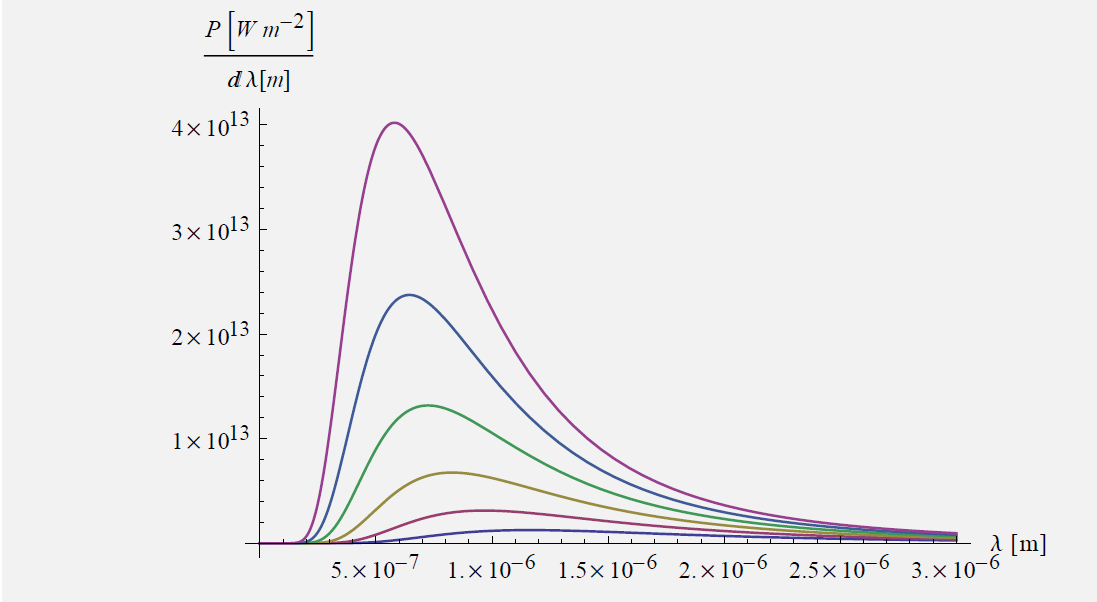
\includegraphics[width=0.7\linewidth]{../images/corpo_nero}
	\caption{Curve di emissione di corpo nero in funzione della lunghezza d’onda a
		diverse temperature (2500K; 3000K; 3500K; 4000K; 4500K; 5000K).}
	\label{fig:corpo_nero}
\end{figure}
\FloatBarrier
Possiamo ora fornire una spiegazione più esaustiva del significato dell'emittanza $\varepsilon$, che è definita come
\[\varepsilon= \frac{f(\lambda)}{f_{cn}(\lambda)}\]
Integrando la funzione di Planck su tutto lo spettro si ottiene la legge di Stefan-Boltzmann per un corpo nero ($\varepsilon = 1$)
\[\int f_{cn}(\lambda)d\lambda = \sigma \theta^4\]
che per un corpo generico va corretta con l'aggiunta di $\varepsilon$. Derivando la funzione di Planck e ponendola uguale a zero si ottiene la lunghezza d'onda in cui l'emissione è massima (a parità di temperatura del corpo che emette), questa soddisfa la relazione
\[\lambda_{max} \theta= 2.9 \cdot 10^{-3}\ m K =cost.\] 
Questa è detta \textbf{legge di Wien}.\\
\'{E} possibile realizzare un corpo nero in laboratorio con un contenitore cubico le cui pareti interne sono rivestite di un materiale nero e su cui viene applicato un piccolo foro su una delle pareti. Si riscalda per irraggiamento il cubo (mettendolo in un forno molto più grande dentro il quale è stato realizzato il vuoto e senza far toccare il cubo con le pareti del forno), la radiazione che penetra nel cubo viene certamente assorbita e la radiazione riemessa dal forellino rispetta la legge di Planck. 
\begin{exercise}[Sistema Terra-Sole]
I dati noti sono:
\begin{itemize}
	\item $k_s = 1350\ W m^{-2}$  (energia che arriva per irraggiamento dal sole sulla cima dell'atmosfera per unità di superficie e di tempo)
	\item $\lambda_{max} = $      (massimo dello spettro solare, corrispondente alla riga giallo-verde)
	\item $R = 7\cdot 10^8\ m$ (raggio del sole)
	\item $r = 6.7\cdot 10^6\ m$ (raggio della terra)
	\item $d = 1.5 \cdot 10^{11}$ (distanza terra-sole)
	\item $a = 0.35 $ (albedo medio della terra, ovvero la riflettanza della terra)
\end{itemize}
e si vuole calcolare (1) se il sole può essere approssimato ad un corpo nero e (2) la temperatura media sulla terra (considerando solo l'irraggiamento del sole).\\
\begin{enumerate}
	\item  Se il sole fosse un corpo nero avremmo $\varepsilon = 1$ e dovrebbero valere contemporaneamente la legge di Wien e quella di Stefan-Boltzmann, le possiamo mettere a sistema
	\begin{align*}
		&\begin{cases}
			\theta = \frac{2.9 \cdot 10^{-3}}{\lambda_{max}} = 5686\ K\\
			\frac{\delta Q}{dt} = 1 \cdot 4\pi R^2\cdot \sigma \theta^4 = 4\pi d^2 k_s
		\end{cases}\\
	&\begin{cases}
		\theta = \frac{2.9 \cdot 10^{-3}}{\lambda_{max}} = 5686\ K\\
		\theta = \sqrt[4]{\frac{d^2 k_s}{R^2 \sigma}} = 5770\ K
	\end{cases}
	\end{align*}
	Come vediamo, i due valori di $\theta$ sono molto simili, ne deduciamo che il sole approssima molto bene un corpo nero (il dato sperimentale è stato inserito nel sistema con \(k_s\), abbiamo poi confrontato la misura sperimentale con quella teorica ottenuta a partire dall'ipotesi di corpo nero ). 
	\item Per conoscere la temperatura della terra imponiamo che l'energia emessa dalla terra è uguale a quella che assorbe dal sole
	\begin{align*}
		&(1-a)\pi r^2 k_s = 1\cdot 4 \pi r^2 \sigma \theta_e^4\\
		&\theta_e = \left[\frac{(1-a)k_s}{4\sigma}\right]^{\frac{1}{4}}\simeq 255\ K \simeq -18\ C
	\end{align*}
dove la radiazione assorbita è uguale a quella che arriva dal sole meno quella riflessa secondo quanto indicato dall'albedo (da qui il coefficiente moltiplicativo \((1-a)\)).\\
Il valore ottenuto è inferiore a quello reale, di circa 288 \textdegree K, poiché non abbiamo tenuto conto dell'effetto serra che, trattenendo all'interno dell'atmosfera le radiazioni infrarosse per riflessione, fa aumentare la temperatura. 
\end{enumerate}
\end{exercise}

\begin{exercise}[Bilancio termico del corpo umano]
	Il corpo umano emette calore con una potenza di circa 110 W a causa del metabolismo basale dell'organismo. Il calore che scambia è dovuto sia all'irraggiamento che alla convezione (visto che l'aria è uno scarso conduttore la conduzione è trascurabile). \'{E} dimostrabile che se un corpo è immerso in un altro (come il corpo umano nell'aria) e la differenza fra le temperature è molto minore della media fra esse (cosa che si avvera per la temperatura ambiente e corporea), la legge che esprime la potenza con cui viene scambiato il calore è (dove $\theta$ è la temperatura corporea e $\theta_{infty}$ quella ambientale)
	\[P  = \frac{\delta Q}{dt} = h A (\theta - \theta_{\infty})\]
	Questo è della stessa forma della legge della convezione, basterà quindi sommarle
	\begin{align*}
		&P  = \frac{\delta Q}{dt} = h_t A (\theta - \theta_{\infty}) + h_c A (\theta - \theta_{\infty}) = H A (\theta - \theta_{\infty})\\
	\end{align*}
	dove $H \equiv h_t + h_c$, $h_c$ è in generale più piccolo di $h_t$.\\
	Ora, conoscendo la temperatura corporea $\theta$, H e A e la potenza con cui emette calore il corpo (che si possono misurare) è possibile ricavare dalla formula precedente la temperatura che dovrebbe avere l'ambiente per essere in equilibrio termico con il corpo umano. ne risulta che la temperatura di equilibrio è di 26 \textdegree C (considerando un corpo nudo), se $\theta_{infty} < 26 C $ bisognerà vestirsi per isolare il copro e diminuire H, se $\theta_{infty} > 26 C $ sia attiveranno i meccanismi di termoregolazione corporei che con la sudorazione raffreddano il corpo poiché l'acqua sulla superficie della pelle evaporando assorbe calore latente di fusione. 
\end{exercise}
\begin{exercise}[Scambio combinato per conduzione ed irraggiamento]
In un sistema come quello in figura, dove un'estremità è stata annerita (ovvero è stata resa un corpo nero) una sbarra di rame isolata sui lati lunghi è a contatto diretto con un termostato a 20 gradi Kelvin ad una estremità ed è riscaldato per irraggiamento da una sorgente a 300 Kelvin dall'estremità in cui è stata annerita. Vogliamo calcolare la differenza di temperatura fra le due estremità.
\begin{figure}[h!]
	\centering
	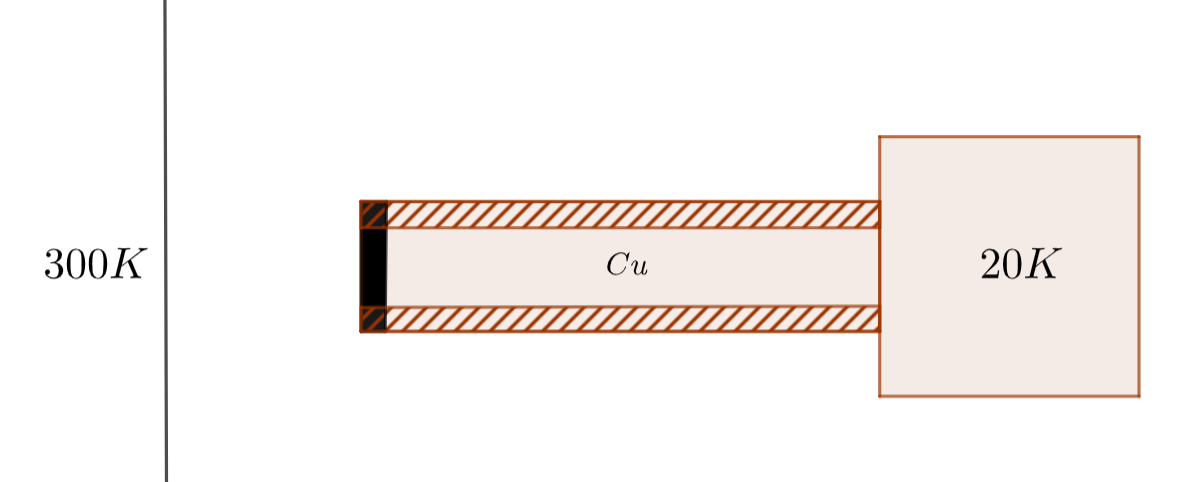
\includegraphics[width=0.6\linewidth]{../images/esercizio_scambio_calore}
	\caption{Schema dell'apparato}
	\label{fig:esercizioscambiocalore}
\end{figure}
\FloatBarrier
La potenza con cui emette in corpo nero all'interno della sbarra di rame è regolato dalla legge di Stefan-Boltzmann, questa deve essere uguale alla potenza con cui assorbe calore, regolata dalla legge di Fourier 
\begin{align*}
	\frac{\delta Q}{dt} = \varepsilon \sigma A \theta^4 = k A \frac{d\theta}{dx}
\end{align*}
Si noti che $\varepsilon = 1$ perché è un corpo nero, dx = L e $d\theta = \Delta\theta$.
\begin{align*}
	&\Delta\theta = \frac{\sigma L \theta^4}{K} \simeq 4.6\cdot 10^{-3}\ K\\
	&\theta_1 = \theta_2 + \Delta\theta \simeq 20.0046\ K
\end{align*}

\end{exercise}

\section{Secondo principio della termodinamica}
\subsection{Paradosso di Loschmidt}
Consideriamo tre esempi di applicazione del primo principio della termodinamica già visti: il blocchetto che scivola su una rampa con attrito, due corpi in contatto che scambiano calore e l'espansione adiabatica di un gas nel vuoto (analogamente all'esperimento di Joule). Il primo principio fornisce informazioni sull'"economia" dell'energia scambiata nelle trasformazioni ma non fornisce alcuna restrizione sulla direzione in cui devono avvenire queste trasformazioni. In altre parole, attenendosi solo al primo principio basterebbe cambiare il segno alle trasformazioni per ottenere, ad esempio, un blocchetto che sale spontaneamente sulla rampa restituendo il calore dissipato per attrito, o il calore che passa da un corpo più freddo ad uno più caldo spontaneamente. \'{E} chiaro che questi fenomeni non si riscontrano nell'esperienza, ciò ci suggerisce la necessità di introdurre un nuovo principio che stabilisca una \textbf{linea del tempo}, infatti la possibilità di invertire le trasformazioni termodinamiche equivarrebbe a "mandare a ritroso" il tempo.\\
Tuttavia, prendendo in esame le leggi fondamentali della fisica, ad esempio la legge di Newton \(F = m \ddot{x}\), risulta che queste sono \textbf{invarianti rispetto al tempo} (o t-invarianti), cioè sono valide sia per t che per -t. Anche se considerassimo le leggi della fisica quantistica, anche queste godono di t-invarianza. Sorge quindi un problema profondo: se a livello microscopico la natura "non distingue tra presente e futuro" perché a livello macroscopico sembra evidente dall'esperienza che vi sia una direzione privilegiata della freccia del tempo (dal passato verso il futuro), testimoniata dall'impossibilità di invertire le trasformazioni termodinamiche. Questo problema è detto \textbf{paradosso di Loschmidt}, alla fine di questa sezione arriveremo a fornire una spiegazione plausibile a questo problema ma è bene tenere a mente che ancora oggi non esiste un consenso generale su questo problema.\\
Si consideri ad esempio un uovo posto sulla superficie di un tavolo, che costituisce lo stato termodinamico A, e lo stesso uovo che, una volta caduto a terra dal tavolo si è frantumato, che costituisce lo stato B. Lo spazio delle fasi di tutti gli atomi che compongono la trasformazione sarà costituito da una curva che congiunge gli stati A e B mediante un percorso $\Gamma$ (ad ogni punto su questo grafico è associato un vettore quantità di moto e uno posizione con 6N componenti ciascuno). Ci chiediamo se, in linea teorica, sia possibile prendere ogni singolo atomo dell'uovo e dell'ambiente circostante, invertire il verso del vettore quantità di moto, e quindi ripercorrere a ritroso la curva $\Gamma$, in questo modo potremmo "mandare a ritroso" la caduta dell'uovo. In teoria la meccanica classica non proibisce tale meccanismo ma ciò è in netta contraddizione con quanto si osserva: in termini della filosofia della scienza, infatti, vi è una propensione del sistema a passare da A a B e non viceversa. In realtà, a livello teorico sarebbe anche possibile riportare gli atomi dell'uovo allo stato iniziale in modo forzato, cioè bisogna che qualcosa nell'ambiente esterno (ad esempio lo sperimentatore) produca questa inversione. L'ambiente esterno deve dunque modificarsi per poter mandare gli atomi del sistema a ritroso: sarebbe dunque impossibile portare sia l'uovo che l'ambiente allo stato iniziale! A causa dell'impossibilità di portare a ritroso una trasformazione termodinamica si postula che non esistano trasformazioni \textbf{reversibili} (ovvero che si possono portare all'indietro) e cioè che tutte le trasformazioni reali sono \textbf{irreversibili}. Questi due concetti sono di fondamentale importanza.\\
Esistono tre coppie di eventi sperimentali discordanti fra mondo microscopico e macrosocopico del tutto equivalenti:
\begin{itemize}
	\item t-invarianza delle leggi fondamentali $\nLeftrightarrow$ freccia del tempo macroscopica
	\item reversibilità microscopica $\nLeftrightarrow$ irreversibilità macroscopica
	\item forze fondamentali tutte conservative $\nLeftrightarrow$ esistenza di forze macroscopiche non conservative
\end{itemize}
L'ultimo punto è esattamente analogo ai primi due infatti possiamo vedere il problema in termini di calore e lavoro: ci chiediamo se sia sempre possibile trasformare tutto il lavoro in calore e tutto il calore in lavoro. Sicuramente trasformare tutto il lavoro in calore è possibile, ad esempio quando si sfregano due pietre sott'acqua; il problema sta nell'inverso. Dal punto di vista teorico, basandosi sul primo principio sarebbe possibile, ad esempio in una trasformazione quasistatica a temperatura costante di un gas perfetto all'interno di un pistone, si ha $\Delta U = 0$ perché la temperatura è costante dunque \(L = Q\).
Si noti che una macchina come un pistone del tipo appena considerato non ha una vera utilità pratica perché non è una trasformazione ciclica: una volta finita l'espansione (facendo un lavoro $L>0$), per tornare allo stato iniziale bisognerà passare inevitabilmente dallo stesso percorso e dunque compiere lo stesso lavoro con segno opposto, il ciclo in totale avrebbe un lavoro pari a zero e dunque sarebbe inutile. Tuttavia, queste sono tutte idealizzazioni che non tengono conto delle forze d'attrito, che per quanto riducibili con varie tecniche non sono mai annullabili. A causa di ciò la trasformazione precedente dissiperebbe sempre una certa quantità di calore e il lavoro totale di un ciclo sarebbe negativo
\begin{align*}
	&L_{andata} = Q-Q_{att}\\
	&L_{ritorno} = -Q-Q_{att}\\
	&L_{tot} = -2Q_{att}
\end{align*}
Dunque in generale in un ciclo di una macchina isoterma si ha \(Q = L \leq 0\) dove è \(Q=L=0\) solo nel caso ideale in cui non vi siano forze non conservative. Il dato sperimentale dell'impossibilità di eliminare le forze non conservative (e dunque l'impossibilità di non dissipare calore in una trasformazione) è stato elevato a principio nella seconda metà del 1800
\subsection{Enunciato di Kelvin-Planck}
\begin{definition}[Definizione di Kelvin-Planck del secondo principio]
	È impossibile realizzare una trasformazione il cui unico risultato sia quello di convertire interamente in lavoro il calore assorbito da un unico serbatoio. In linguaggio matematico: in una trasformazione in cui $\Delta U =$ costante allora \(L = Q_1+Q_2 = |Q_1| - |Q_2|> 0\) dove $Q_1$ è il calore assorbito dalla macchina (> 0)e $Q_2$ il calore dissipato (< 0).
\end{definition}
\begin{figure}[h!]
	\centering
	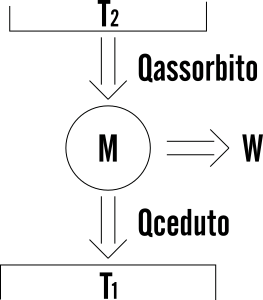
\includegraphics[width=0.3\linewidth]{../images/macchina-termica}
	\caption{Schema della macchina termica minimale.}
	\label{fig:macchina-termica}
\end{figure}
\FloatBarrier
Si noti che per effettuare una trasformazione ciclica servono sempre almeno due serbatoi perché, come visto, se ci fosse solo un serbatoio (temperatura costante) l'area del ciclo sarebbe nulla. Dunque questo principio stabilisce l'impossibilità el moto perpetuo di seconda specie ovvero di sfruttare unicamente una fonte di calore, potenzialmente di capacità termica infinita (come il mare o l'aria) per creare lavoro. Parte del calore non viene convertito ma sprecato, dissipandosi in un serbatoio più freddo. \\
Visto che non tutto il calore può essere trasformato in lavoro, possiamo definire l'efficienza come la frazione di calore assorbita convertita in lavoro utile
\begin{align*}
	\eta = \frac{L}{Q_1} = \frac{Q_1 + Q_2}{Q_1} = 1 + \frac{Q_2}{Q_1} = 1- \frac{|Q_2|}{|Q_1|}< 1
\end{align*}
Quest'ultima disuguaglianza è un'altra forma della definizione del secondo principio della termodinamica secondo Kelvin-Planck. Nel caso di macchine politermiche, cioè che lavorano in presenza di più di due termostati, l'efficienza è 
\[\eta = \frac{L}{\sum_i Q_{abs}}\]
\subsubsection{Macchina di Stirling}
A parità di sorgenti è possibile costruire infinite macchine termiche con cicli termodinamici e rendimenti diversi. Consideriamo la macchina di Stirling, un ciclo reversibile composto da due isoterme e due isocore. 
\begin{figure}[h!]
	\centering
	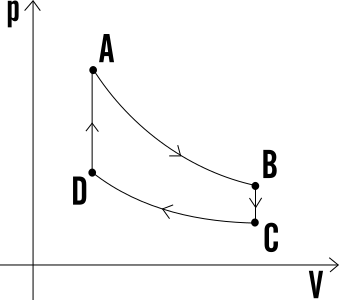
\includegraphics[width=0.4\linewidth]{../images/ciclo_di_stirling}
	\caption{Grafico sul piano di Clapeyron di un ciclo di Stirling}
	\label{fig:ciclodistirling}
\end{figure}
\FloatBarrier
Questo tipo di macchina è detta a "combustione esterna", cioè funziona con una sorgente di calore esterna al sistema. Si fa inoltre uso di un sistema esterno rigeneratore R, ovvero un sistema ausiliario che nella fase di andata accumula calore che viene restituito nella fase di ritorno. Questo rigeneratore R aiutò Stirling ad aumentare l'efficienza della sua macchina rispetto a quelle del tempo. Vogliamo calcolare il rendimento di questa macchina, cominciamo con il rilevare che nella trasformazione AB assorbe calore, BC lo emette, CD lo emette e DA lo assorbe. 
\begin{align*}
&\eta = \frac{L}{Q_{abs}} = \frac{L}{Q_1 + Q_R}\\
&L_{AB}= n R \theta_1 \ln\left(\frac{V_b}{V_a}\right)\\
&L_{CD}= n r \theta_2 \ln\left(\frac{V_d}{V_c}\right) = n r \theta_2 \ln\left(\frac{V_b}{V_a}\right)\\
&L = L_{AB} + L_{CD} = n R \ln\left(\frac{V_b}{V_a}\right)(\theta_1 - \theta_2)\\
&Q_1 = n R \ln\left(\frac{V_b}{V_a}\right)(\theta_1 - \theta_2)\\
&Q_R = n c_v (\theta_1 - \theta_R)\\
&\eta = \frac{L}{Q_{abs}} = \frac{L}{Q_1 + Q_R} = \frac{R \ln\left(\frac{V_b}{V_a}\right)(\theta_1 - \theta_2)}{R\theta_1\ln(\frac{V_b}{V_a})+c_v (\theta_1 - \theta_2)}
\end{align*}
\subsubsection{Ciclo Otto}
Questo ciclo termodinamico a combustione interna, tipicamente usato nei motori a benzina che sfrutta l'utilizzo di una candela per far esplodere il fluido ed ottenere un'espansione adiabatica (visto che esplode l'espansione avviene tanto rapidamente da non scambiare calore con l'ambiente). \'{E} caratterizzato da due adiabatiche chiuse da due isocore, come in figura.
\begin{figure}[h!]
	\centering
	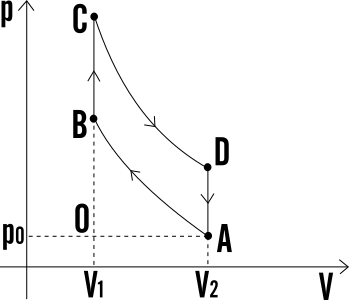
\includegraphics[width=0.4\linewidth]{../images/ciclo-otto}
	\caption{Grafico del ciclo otto. AB e CD sono curve adiabatiche, BC e DA curve isocore.}
	\label{fig:ciclo-otto}
\end{figure}
\FloatBarrier
vogliamo ricavare il rendimento di questo ciclo. Osservando che il calore viene assorbito solamente nel tratto isotermo DA ($Q_1$) , possiamo scrivere
\begin{align*}
 &\eta = \frac{L}{Q_{abs}}
\end{align*} 
Ipotizziamo che il gas all'interno della macchina sia perfetto, sappiamo che il lavoro di un'isocora è nullo e conosciamo quello di un'adiabatica per un gas perfetto; inoltre sappiamo che il calore è assorbito unicamente nell'isocora CB ed è uguale alla variazione di energia interna del gas perfetto (essendo un'isocora), che conosciamo.
\begin{align*}
	&L =n c_v (\theta_C-\theta_D) + n c_v(\theta_A-\theta_B)\\
	&Q_{abs} = \Delta U = n c_v (\theta_C-\theta_B)\\
	&\eta = \frac{n c_v (\theta_C-\theta_D) + n c_v(\theta_A-\theta_B)}{n c_v (\theta_C-\theta_B)} = \frac{(\theta_C-\theta_D + \theta_A-\theta_B)}{(\theta_C-\theta_B)} = 1 - \frac{\theta_D - \theta_A}{\theta_C - \theta_B}
\end{align*}
 Sfruttiamo ora la proprietà delle adiabatiche che mette in relazione temperatura e volume
 \begin{align*}
 &\begin{cases}
 	&\theta_C V_1^{\gamma-1} = \theta_D V_2^{\gamma-1}\\
 	&\theta_B V_1^{\gamma-1} = \theta_A V_2^{\gamma-1}
 \end{cases}\\
& \Rightarrow \frac{\theta_C}{\theta_B} = \frac{\theta_D}{\theta_A}ù \quad \frac{\theta_D}{\theta_C}=\frac{V_2^{\gamma-1}}{V_1^{\gamma-1}}\\
&\eta = 1 - \frac{\theta_D}{\theta_C}\left(\frac{1-\frac{\theta_A}{\theta_D}}{1-\frac{\theta_B}{\theta_C}}\right) = 1-\frac{\theta_D}{\theta_C} = 1-\frac{V_2^{\gamma-1}}{V_1^{\gamma-1}}
\end{align*}
\subsubsection{Ciclo Diesel}
Il ciclo Diesel è un ciclo termodinamico per motori a combustione interna dove, a differenza del ciclo Otto, l'accensione della miscela non avviene attraverso una candela bensì per effetto dell'alta temperatura conseguente alla fase di compressione. Esso comprende 4 fasi o trasformazioni. L'idea di tale macchina termica fu di Rudolf Diesel che sviluppò successivamente il motore Diesel. \'{E} caratterizzato da due adiabatiche chiuse da un'isobara e un'isocora, come in figura
\begin{figure}[h!]
	\centering
	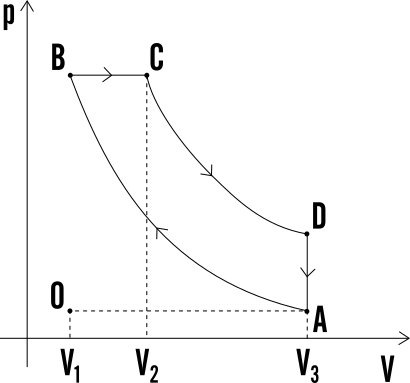
\includegraphics[width=0.4\linewidth]{../images/ciclo-diesel}
	\caption{Grafico del ciclo Diesel. CD e AB sono due adiabatiche, DA è un'isocora e BC un'isobara}
	\label{fig:ciclo-diesel}
\end{figure}
\FloatBarrier
Vogliamo ricavare il rendimento. L'unica trasformazione in cui si assorbe calore è l'isobara, l'unica in cui si cede è l'isocora
\begin{align*}
	&\eta = \frac{L}{Q_{abs}} = \frac{Q_{abs}+Q_{ced}}{Q_{abs}} = 1 +\frac{Q_{ced}}{Q_{abs}} = 1 + \frac{c_v(\theta_A-\theta_D)}{c_p(\theta_C-\theta_B)} = 1+\frac{1}{\gamma}\frac{(\theta_A-\theta_D)}{(\theta_C-\theta_B)} = 1 - \frac{(\theta_D-\theta_A)}{(\theta_C-\theta_B)}
\end{align*}
\subsection{Enunciato di Clausius}
\begin{definition}[Macchina frigorifera]
	Viene detta macchina frigorifera una macchina che fa lavoro per trasferire calore da corpi più freddi a corpi più caldi. 
\end{definition}
\begin{definition}[Enunciato del secondo principio secondo Clausius]
	\'{E} impossibile ottenere una trasformazione che come unico risultato abbia quello di trasferire calore da un corpo più freddo ad uno più caldo. 
\end{definition}
Vista la definizione di macchina frigorifera, si deduce che questo principio vieta l'esistenza una macchina frigorifera che porti calore da un corpo freddo ad uno caldo senza fare lavoro. 
\begin{figure}[h!]
	\centering
	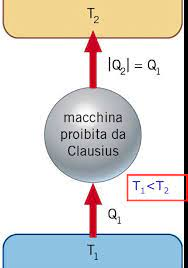
\includegraphics[width=0.35\linewidth]{../images/clausius}
	\caption{Schema della macchina frigorifera proibita dall'enunciato di Clausius.}
	\label{fig:clausius}
\end{figure}
\FloatBarrier
Possiamo definire, analogamente al rendimento per una macchina termica, il coefficiente di prestazione per una macchina frigorifera
\begin{definition}[coefficiente di prestazione]
	Definiamo il coefficiente di prestazione di una macchina frigorifera come \[\omega =\equiv \frac{Q_2}{|L|} = \frac{Q_2}{|Q_1|-|Q_2|}\]
\end{definition}
Dimostriamo ora che l'enunciato di Kelvin-Planck (KP) e quello di Clausius (C) sono equivalenti. Preliminarmente, svolgiamo alcune considerazioni logiche.
\begin{align*}
	&KP \Leftrightarrow C\\
	&\begin{cases}
		KP \Rightarrow C\\
		C \Rightarrow KP
	\end{cases}\\
	&\begin{cases}
		\neg(KP)\Rightarrow \neg(C)\\
		\neg(C)\Rightarrow \neg(KP)
	\end{cases}
\end{align*}
Dunque basta dimostrare che la negazione di uno implica la negazione dell'altro per dimostrare l'equivalenza dei due enunciati. Si noti che negare uno dei due enunciati equivale ad ammettere l'esistenza di una macchina che contravvenga all'enunciato. 
\begin{enumerate}
	\item \(\neg(KP)\Rightarrow \neg(C)\)\\
	
	Neghiamo KP costruendo una macchina termica che lo neghi ed uniamola ad una macchina frigorifera che rispetti C, otteniamo una macchina come in figura
\begin{figure}[h!]
	\centering
	\includegraphics[width=0.5\linewidth]{../images/KP-C}
	\caption{Schema dell'unione di una macchina che contravviene l'enunciato KP (perché non scambia calore con il secondo serbatoio) a sinistra con una che rispetta l'enunciato C a destra (perché per funzionare assorbe il calore proveniente dalla prima macchina). La seconda macchina è costruita in modo che \(Q_C = Q_A + Q_{A2}\)}
	\label{fig:kp-c}
\end{figure}
\FloatBarrier
Questa macchina nella sua totalità è equivalente ad una macchina \(M_1 + M_2\) che assorbe calore \(Q_{A2}\) e ne cede \(-Q_A+Q_C\), dove $Q_C = Q_{A}+Q_{A2}$ dunque in totale cede \(Q_{A2}\). Il lavoro prodotto dalla prima macchina è lo stesso assorbito dalla seconda con segno invertito dunque il lavoro totale prodotto/assorbito è nullo. Abbiamo così ottenuto un macchina che come unico effetto ha quello di assorbire calore da una sorgente più fredda e portarlo ad una più calda, che equivale ad una macchina che nega l'enunciato di Clausius.

\item \(\neg(C)\Rightarrow \neg(KP)\)\\

Costruiamo una macchina che nega l'enunciato di Clausius, ovvero che porta calore da una sorgente fredda ad una calda senza fare lavoro, e la uniamo ad una macchina che rispetta l'enunciato di KP come in figura.
\begin{figure}[h!]
	\centering
	\includegraphics[width=0.5\linewidth]{../images/C-KP}
	\caption{Schema dell'unione di una macchina che nega l'enunciato di C con una che rispetta quello di KP. Si noti che la seconda macchina è stata costruita in modo da assorbire la stessa quantità di calore che la prima trasferisce (in figura \(Q = Q_A\) }
	\label{fig:c-kp}
\end{figure}
\FloatBarrier
Visto che la seconda macchina espelle calore e lavoro, per la conservazione dell'energia \(Q_C<Q_A=Q\).
Unire queste due macchine equivale ad avere una macchina che assorbe \(Q-Q_C = Q' > 0 \) ed espelle \(Q-Q_A = 0\) producendo lavoro W. Questa macchina prende calore da una sola sorgente e produce lavoro, contraddice dunque l'enunciato di KP.  
\end{enumerate} 
\subsubsection{Ciclo di Carnot}
Il ciclo formato da due isoterme chiuse da due adiabatiche, come in figura, è detto \textbf{ciclo di Carnot}. Ogni sostanza ha un ciclo di Carnot diverso poiché la forma delle adiabatiche e delle isoterme dipendono dalle caratteristiche chimiche dei materiali. 
\begin{figure}[h!]
	\centering
	\includegraphics[width=0.5\linewidth]{../images/ciclo_carnot}
	\caption{Schema del ciclo di Carnot, le trasformazioni AB e CD sono due isoterme, BC e DA sono adiabatiche.}
	\label{fig:ciclocarnot}
\end{figure}
\FloatBarrier
Questo è un ciclo particolare perché è dimostrabile che sia quello con rendimento maggiore, a parità di serbatoi termici con i quali si opera. 
\begin{theorem}[Teorema di Carnot]
	Il rendimento di una macchina termica M che opera tra o con due serbatoi termici è sempre minore o uguale al rendimento della macchina di Carnot corrispondente.
	\[\eta \leq \eta_c\]
\end{theorem}
Per dimostrare questo teorema consideriamo una macchina termica M qualsiasi che assorbe Q da una sorgente calda a $\theta_1$ producendo un lavoro $L_m$ ed emette calore $Q-L_m$ ad un serbatoio a temperatura $\theta_2$. Consideriamo inoltre una macchina di Carnot C che assorbe Q dalla stessa sorgente calda a $\theta_1$ producendo un lavoro $L_c$ ed emette calore $Q-L_m$ ad un serbatoio a temperatura $\theta_2$. Vista l'invertibilità di una macchina di Carnot, possiamo trasformarla in una macchina frigorifera semplicemente cambiando i segni dei calori emessi/assorbiti e del lavoro emesso/assorbito. Otteniamo così una macchina $\overline{C}$ che possiamo unire alla macchina M, il calore scambiato con il serbatoio a $\theta_1$ è \(Q-Q = 0\) mentre con quello a $\theta_2$ scambia \(Q-L_m - (Q-L_c) = L_c-L_m\) e assorbe/produce lavoro pari a \(L_m-L_c\). Non sapendo quale sia maggiore tra \(L_c\) ed \(L_m\) non sappiamo in che direzione fluisca il calore e se il lavoro venga prodotto o assorbito. sappiamo tuttavia, per il secondo principio secondo Kelvin Planck che non può esistere una macchina che trasforma tutto il calore prelevato da un'unica sorgente in lavoro (impedisce dunque un verso) ne deduciamo che sarà il lavoro ad essere trasformato in calore, allora \[L_m-L_c \leq 0 \Rightarrow L_m \leq L_c\] Abbiamo così dimostrato che, a parità di temperature dei serbatoi tra o con cui opera una macchina generica ed una di Carnot, il lavoro di quest'ultima sarà sempre maggiore. Dividendo per Q ambo i membri e ricordando la definizione di rendimento
\[\frac{L_m }{Q} \leq \frac{L_c}{Q} \Rightarrow \eta_m \leq \eta_c\]
Dove la condizione di uguaglianza si verifica solo se anche $\eta_m$ è una macchina di Carnot.
\begin{corollary}[Tutte le macchine di Carnot hanno lo stesso rendimento]
Come dimostrato dal teorema di Carnot, il rendimento della macchina di Carnot è il maggiore ottenibile da una macchina termica. Date due macchine di Carnot C1 e C2 considerando C1 macchina termica qualsiasi e C2 macchina di Carnot abbiamo \[\eta_{c1}\leq \eta_{c2}\] Se contrariamente consideriamo C1 macchina di Carnot e C2 macchina termica generica, otteniamo \[\eta_{c1}\geq \eta_{c2}\] Mettendo a sistema le due precedenti relazioni si ottiene \[\eta_{c1} = \eta_{c2}\] Da cui si ricava che due macchine di Carnot qualsiasi hanno lo steso rendimento. 
\end{corollary}

A causa di questo corollario, notiamo che qualunque materiale venga usato in una macchina di Carnot, questa avrà sempre lo stesso rendimento che dipende unicamente da $\theta_1$ e $\theta_2$. 
\[\eta_ c= f(\theta_1\ ,\theta_2 )\]
Vogliamo calcolare f, visto che questa è indipendente dal tipo di materiale usato, adottiamo un gas perfetto per semplicità. 
\begin{align*}
	\eta_c = \frac{L}{Q}=\frac{Q_1 + Q_2}{Q_1}= 1 + \frac{Q_2}{Q_1}
\end{align*} 
Calcoliamo \(Q_1\) e \(Q_2\). \(Q_1\) è il calore assorbito nella trasformazione AB, come in figura. Visto che è una trasformazione isoterma si ha \(\Delta U = 0 \Rightarrow L_{AB}  = Q_1\). Sappiamo calcolare il lavoro di un gas perfetto in un'isoterma, per semplicità consideriamo solamente una mole. Analogamente ad AB procediamo con CD
\begin{align*}
	&Q_1 = L_{AB} = R\theta_1\ln(\frac{V_B}{V_A})\\
	&Q_2 = L_{CD} = R\theta_2\ln(\frac{V_D}{V_C})
\end{align*}
Nelle adiabatiche invece $Q=0$. Dalle precedenti si ricava
\begin{align*}
	\eta_C = 1+\frac{\theta_1\ln(\frac{V_B}{V_A})}{\theta_2\ln(\frac{V_D}{V_C})}
\end{align*}
Visto che gli stati B-C e A-D sono legati da trasformazioni adiabatiche, possiamo sfruttare le relazione 
\begin{align*}
	&\begin{cases}
		\theta_1 V_B^{\gamma -1} = \theta_2 V_C^{\gamma -1}\\
		\theta_1 V_A^{\gamma -1} = \theta_2 V_D^{\gamma -1}
	\end{cases}
	\Rightarrow \frac{V_B}{V_A} = \frac{V_C}{V_D}\\
	&\Rightarrow \eta_C = 1-\frac{\theta_1}{\theta_2}
\end{align*}
Possiamo anche ricavare il coefficiente di prestazione $\omega$ di un macchina frigorifera di Carnot. 
\begin{align*}
\omega = \frac{Q_2}{|L|} = \frac{Q_2}{|Q_1|-|Q_2|} = \frac{\theta_2}{\theta_1 - \theta_2}
\end{align*}
\section{Ridefinizione della temperatura con il ciclo di Carnot}
Come visto in precedenza, il simbolo $\theta$ indica la temperatura definita mediante il termometro a gas perfetto: un corpo ha una temperatura $\theta$ se la grandezza indicata dal termometro a gas perfetto posto in equilibrio termico con tale corpo è di $\theta$. Questa definizione ha il limite di appellarsi ad un gas che, a temperature troppo basse, inevitabilmente fonde (la minima temperatura di fusione è 0.5K per l'$H^3$). Per temperature minori a 0.5 K non possiamo definire la temperatura.\\
Eliminiamo dunque la definizione della temperatura mediante i gas perfetti e torniamo al punto di partenza in cui avevamo grandezze "t", prive di scala termometrica. Vogliamo sfruttare la relazione \[\eta_c = 1+\frac{|Q_2|}{|Q_1|}=f(t_1,t_2) \Rightarrow \frac{|Q_2|}{|Q_1|}=f(t_1,t_2)\]
per ridefinire la temperatura. Consideriamo due macchine di Carnot C1 e C2 operanti una tra $t_0$ e $t_1$ e l'altra tra $t_0$ e $t_2$. La prima assorbe calore \(Q_1\) dal serbatoio a \(t_1\), produce lavoro \( L_1\) e restituisce calore \(Q_0\) al serbatoio \(t_0\), analogamente la seconda preleva \(Q_2\) da \(t_2\), produce \(L_2\) e cede \(Q_0\) a \(t_0\). Sappiamo che
\begin{align*}
	&\frac{|Q_1|}{|Q_0|} =f(t_1\ , t_0) \quad \frac{|Q_2|}{|Q_0|} =f(t_2\ , t_0)\\
	&\Rightarrow \frac{|Q_2|}{|Q_1|} =\frac{f(t_1\ , t_0)}{f(t_2\ , t_0)}
\end{align*}
Ora, posso invertire C1 invertendo i segni e trasformandola in una macchina frigorifera di Carnot $\overline{C1}$. Avremo dunque che $\overline{C1}$ assorbe \(Q_0\) da \(t_0\), assorbe lavoro \(L_1\) e cede calore \(Q_1\) a \(t_1\). Unendo le due macchine otterremo una macchina ($\overline{C1}+C2$) che sarà indipendente dal serbatoio a \(t_0\) poiché scambia calore \(Q_0-Q_0 =  0\) e che assorbe calore \(Q_2\) da \(t_2\) e ne cede \(Q_1\) a \(t_1\). Possiamo quindi scrivere
\begin{align*}
&\frac{|Q_1|}{|Q_2|} = f(t_1\ ,t_2)\\
&\Rightarrow f(t_1\ , t_2) = \frac{f(t_1\ ,t_0)}{f(t_2\ ,t_0)}
\end{align*}
Dove nell'ultimo passaggio abbiamo uguagliato con quanto ottenuto appena sopra. data questa uguaglianza è necessario che \(t_0\) sia fattorizzabile da f per poterlo semplificare dunque
\begin{align*}
&\frac{|Q_1|}{|Q_2|} = f(t_1\ , t_2) = \frac{f(t_1\ ,t_0)}{f(t_2\ ,t_0)}= \frac{T(t_1)\Psi(t_0)}{T(t_2)\Psi(t_0)}=\frac{T(t_1)}{T(t_1)}
\end{align*}
Possiamo ridefinire la temperatura come la funzione T: \[T \equiv T(t)\]
possiamo ora fissare la temperatura $T(t_2)\equiv T_3$ come la temperatura del punto triplo dell'acqua e il calore \(Q_2\equiv Q_3\) come il calore scambiato fra il corpo a temperatura del punto triplo con la macchina di Carnot dove invece \(Q_1\equiv Q\) è il calore scambiato tra la macchina di Carnot ed il corpo a temperatura incognita \(T(t_1)\equiv T_x\). 
\[T_x = T_3\frac{|Q|}{|Q_3|}\]
Ecco ottenuta una definizione del calore dipendente solamente dai calori scambiati da due corpi con la macchina di Carnot, e quindi indipendenti dal materiale usato per la misurazione. Abbiamo dunque risolto il problema della definizione di temperature inferiori a \(0.5 K\). 
\section{La disuguaglianza di Clausius}
Confrontiamo il rendimento di una macchina termica generica ed una di Carnot, ricordando che per il thm. di Carnot \(\eta \leq \eta_c\)
\begin{align*}
	&\eta = 1 + \frac{Q_2}{Q_1} \quad \eta_c = 1 - \frac{T_2}{T_1}\\
	&1 + \frac{Q_2}{Q_1} \leq \eta_c = 1 - \frac{T_2}{T_1}\\
	&\Rightarrow \frac{Q_2}{T_2}+\frac{Q_1}{T_1}\leq 0
\end{align*}
Dove l'uguaglianza si avvera se la macchina è di Carnot. Se al posto di avere due termostati ne avessimo n (macchina politermica) come si modificherebbe questa disuguaglianza? Una macchina politermica può essere schematizzata come in figura
\begin{figure}[h!]
	\centering
	\includegraphics[width=0.6\linewidth]{../images/macchina_polit}
	\caption{Schema di una macchina politermica}
	\label{fig:macchinapolit}
\end{figure}
\FloatBarrier
Sommando  tutte le macchine otteniamo una macchina singola (\(M_g+\sum_i^n C_i\)) che opera con un unico serbatoio termico, \(T_0\) e che produce/assorbe lavoro; si tratta di determinare il verso del lavoro e dello scambio di calore. Per il secondo principio secondo KP una macchina che assorbe calore da un unico serbatoio producendo calore non può esistere dunque il verso obbligato è quello in cui la macchina trasforma il lavoro in calore che emette al serbatoio \(T_0\). Ne risulta che il calore scambiato con il serbatoio ha segno negativo dunque 
\[\sum_i Q'_i \leq 0\]
Per ogni macchina di Carnot che forma la macchina politermica vale 
\[Q'_i = T_0 \frac{Q_i}{T_i}\]
Dunque sommando tutti gli n calori scambiati dalle macchine di Carnot si ottiene
\begin{align*}
	&\sum_i Q'_i = \sum_i\frac{T_0 Q_i}{T_i}\leq 0\\
	&\Rightarrow \sum_i \frac{Q_i}{T_i}\leq 0
\end{align*}
Per un numero infinito di macchine di Carnot (e quindi di termostati con cui lavora la macchina politermica) è possibile passare al continuo sostituendo la sommatoria all'integrale. Visto che il grafico di una macchina, in un piano di Clapeyron è una linea chiusa avremo un integrale su un percorso chiuso, ovvero una circuitazione, possiamo dunque scrivere
\begin{align*}
	\oint \frac{\delta Q}{T}\leq 0
\end{align*}
\subsection{Completamento del teorema di Carnot}
Il teorema di Carnot per come abbiamo visto si limita a fornire informazioni su una macchina reversibile che opera tra o con due serbatoi. Vogliamo ora estendere il teorema a macchine reversibili che lavorano con infiniti serbatoi e dimostrare che comunque il rendimento è minore di quello di una macchina di Carnot che lavora fra o con le stesse temperature minima e massima.\\
Consideriamo una trasformazione ciclica continua qualsiasi che lavora fra due isoterme \(T_1\) e \(T_2\) e approssimiamola con un numero discreto di cicli di Carnot come in figura, l'approssimazione è fatta in modo che il calore scambiato sia lo stesso di quello nel tratto di ciclo continuo corrispondente
\begin{figure}[h!]
	\centering
	\includegraphics[width=0.6\linewidth]{../images/ciclo_continuo}
	\caption{Schema dell'approssimazione di un ciclo continuo mediante un numero discreto di cicli di Carnot (due adiabatiche e due isoterme).}
	\label{fig:ciclocontinuo}
\end{figure}
\FloatBarrier
Detto \(Q_i\) il calore scambiato nell'isesimo ciclo di Carnot abbiamo, per la relazione ricavata in precedenza
\begin{align*}
	&\sum_i \frac{Q_i}{T_i} = 0\\
	&\oint \frac{\delta Q}{T} = 0
\end{align*}
Possiamo dividere il calore scambiato nel ciclo in una componente positiva (AB) in cui viene ricevuto ed una negativa (BA) in cui viene ceduto; possiamo dunque scrivere
\begin{align*}
	&\oint \frac{\delta Q}{T} = \int_A^B \frac{|\delta Q_r|}{T}- \int_B^A \frac{|\delta Q_c|}{T}= 0\\
	&\Rightarrow \int_A^B \frac{|\delta Q_r|}{T} = \int_B^A \frac{|\delta Q_c|}{T}
\end{align*}
Visto che per ipotesi \(T_1\) e \(T_2\) sono le temperature estreme, \(T_2<T<T_1 \Rightarrow \frac{1}{T_2}>T>\frac{1}{T_1}\).
\begin{align*}
	&\int_A^B \frac{|\delta Q_r|}{T_1} < \int_A^B \frac{|\delta Q_r|}{T} = \int_B^A \frac{|\delta Q_c|}{T} < \int_B^A \frac{|\delta Q_c|}{T_2}\\
	&\frac{1}{T_1} \int_A^B |\delta Q_r| < \frac{1}{T_2} \int_B^A |\delta Q_c|\\
	&\frac{T_2}{T_1} < \frac{|Q_c|}{|Q_r|}\\
	&\Rightarrow 1-\frac{T_2}{T_1} = \eta_c < \eta_m = 1-\frac{|Q_c|}{|Q_r|}
\end{align*} 
ciò dimostra il teorema di Carnot per macchine che lavorano tra infiniti serbatoi di calore. 
\section{L'entropia}
Torniamo a considerare un ciclo continuo reversibile che va dallo stato A a quello B e vice versa. Distinguiamo il tratto reversibile da A a B \(R_1\) ed \(R_2\) da B ad A. Questi percorsi sono del tutto generici, come lo sono gli estremi A e B. 
\begin{align*}
	&\oint \frac{\delta Q}{T} = \left(\int_A^B\right)_{R_1} \frac{\delta Q}{T} + \left(\int_B^A\right)_{R_2} \frac{\delta Q}{T} = 0
\end{align*}
Essendo trasformazioni reversibili possiamo invertire \(R_2\) semplicemente cambiando il segno
\begin{align*}
	&\left(\int_B^A\right)_{R_2}  \frac{\delta Q}{T} = -\left(\int_A^B\right)_{R_2}  \frac{\delta Q}{T}\\
	&\Rightarrow \left(\int_B^A\right)_{R_1}  \frac{\delta Q}{T} = \left(\int_A^B\right)_{R_2} 
\end{align*}
Vista l'arbitrarietà dei percorsi e degli stati iniziali e finali, se ne deduce che, qualunque essi siano, la grandezza \(\frac{\delta Q}{T}\) dipende unicamente dagli stati iniziali e finali della trasformazione. Possiamo quindi definire una nuova variabile di stato: l'\textbf{entropia}. Definiamo l'entropia di uno stato come 
\begin{align*}
	S(A) = \int_0^A \frac{\delta Q}{T}
\end{align*}
dove è arbitrario scegliere il punto in cui \(S(0)=0\). Questo procedimento è del tutto analogo al calcolo dell'energia interna o dell'energia potenziale gravitazionale (anch'esse variabili di stato) in cui il punto in cui la variabile è nulla è arbitrario. Ciò non è rilevante perché solitamente di parla di variazione di entropia e al costante si elimina
\begin{align*}
	\Delta S_{AB} = \int_A^B \frac{\delta Q}{T}
\end{align*}
dove la trasformazione che va da A a B è reversibile.\\
Consideriamo ora il caso di un ciclo irreversibile, formato da un tratto AB irreversibile ed uno BA reversibile. Abbiamo
\begin{align*}
	&\oint =\left( \int_B^A\right)_R \frac{\delta Q}{T} + \left(\int_A^B\right)_I \frac{\delta Q}{T}=\left(\int_B^A \right)_I \frac{\delta Q}{T} - \Delta S < 0\\
	&\Delta S > \left(\int_B^A\right)_I \frac{\delta Q}{T}\\
\end{align*}
Si noti che se la trasformazione è adiabatica la variazione di entropia è nulla perché non si hanno scambi di calore \((\delta Q = 0)\). \\
Dunque, se un sistema è isolato termicamente ed evolve spontaneamente, se effettua trasformazioni reversibili l'entropia dell'universo resta costante, se ne fa di irreversibili l'entropia aumenta. Ne segue che l'entropia dell'universo tende ad aumentare finché possibile. Visto che quella delle trasformazioni perfettamente reversibili è un'idealizzazione, l'entropia di qualsiasi trasformazione reale aumenta dunque 
\begin{align*}
	\Delta S_U = \Delta S_A + \Delta S_S > 0
\end{align*}
Nonostante l'entropia del sistema o dell'ambiente possano essere singolarmente minori di zero, la loro somma deve sempre essere positiva. 
\subsection{Irreversibilità ed entropia}
Basandoci sul fatto appena ricavato che l'entropia dell'universo deve aumentare, proviamo che i tre casi già visti in precedenza di esempi di trasformazioni termodinamiche irreversibili non possono avvenire in senso opposto (altrimenti l'entropia dell'universo diminuirebbe). 
\subsubsection{Espansione libera}
Riprendiamo il caso della scatola isolata divisa in due setti uguali inizialmente chiusi con un gas perfetto in un setto ed il vuoto nell'altro (stato A), dove la trasformazione termodinamica consiste nell'aprire il setto e lasciare il gas espandersi liberamente. Vogliamo dimostrare che la variazione di entropia è positiva. Per calcolare la variazione d'entropia sfrutto la definizione e scelgo una qualsiasi trasformazione reversibile che porti dallo stato A a quello B; la compressione isoterma (mettendo a contatto il sistema con un termostato) è il caso più semplice. 
\begin{align*}
	&\Delta S = \int_{A}^{B}\frac{\delta Q}{T} = nR\int_{V_a}^{V_b}\frac{dV}{V} =nR\ln\left(\frac{V_b}{V_a}\right)= nR\ln(2)>0
\end{align*}
\subsection{Sistema rampa e blocco}
La trasformazione in cui il blocco scende dalla rampa con attrito è irreversibile quindi dobbiamo trovare una trasformazione reversibile che porti dallo stato A a quello B. Scegliamo quella in cui il blocchetto viene spostato in modo quasistatico dalla posizione in A a quella in B e poi viene riscaldato quasistaticamente iniettandovi calore in modo estremamente lento. Essendo la trasformazione reversibile l'entropia dell'universo deve essere nulla ma l'entropia del sistema deve aumentare. Visto che il calore viene iniettato dall'ambiente verso il sistema, la variazione di calore del sistema sarà positiva e così l'entropia. 
\subsection{Passaggio di calore}
Consideriamo due corpi che allo stato A sono a temperatura \(T_1\), \(T_2\) tali che \(T_2<T_1\)  con rispettive capacità termiche \(c_1\) e \(c_2\). Una volta messi a contatto la temperatura all'equilibrio (stato B) sarà
\[T_e=\frac{c_1T_1 + c_2T_2}{c_1+c_2}\]
La variazione di entropia dell'universo equivale alla variazione di entropia dei due corpi sommata
\begin{align*}
	&\Delta S_1 = \int_{A}^{B}\frac{\delta Q}{T} = \int_{T_1}^{T_e}\frac{c_1 dT}{T}=c_1 \ln\left(\frac{T_e}{T_1}\right)\\
	&\Rightarrow \Delta S_U = \Delta S_1 + \Delta S_2 = c_1 \ln\left(\frac{T_e}{T_1}\right) + c_2 \ln\left(\frac{T_e}{T_2}\right)
\end{align*}
Vogliamo dimostrare che quest'ultima quantità sia maggiore di zero. Analizziamo due casi particolari in cui la dimostrazione è particolarmente semplice
\subsubsection{\(c_1=c_2\)}
\begin{align*}
	&\Delta S_U = c\left(\ln\left(\frac{T_e^2}{T_1T_2}\right) \right) = c\left(\ln\left(\frac{(\frac{T_1 + T_2}{2})^2}{T_1T_2}\right) \right)=\\
	&c\left(\ln\left(\frac{(T_1 + T_2)^2}{4T_1T_2}\right) \right)=c \ln\left[1 + \frac{(T_1 - T_2)^2}{4T_1T_2}\right]>0
\end{align*}
\subsubsection{\(c_1>>c_2\)}
Definiamo \(r \equiv \frac{c_2}{c_1}>>1\) e \(R \equiv \frac{T_2}{T_1}\)
\begin{align*}
	&T_e = \frac{T_1 + r T_2}{1+r}= \frac{1+rR}{1+r}T_1\\
	&\Delta S_1 = c_1 \ln\left(\frac{T_e}{T_1}\right) = c_1 \ln\left(\frac{1+rR}{1+r}\frac{T_1}{T_1}\right)\\
	&\simeq c_1(R-1)r = c_1(\frac{T_2}{T_1}-1) \frac{c_2}{c_1} = \frac{c_2 (\Delta T)}{T_1} = -\frac{|c_2\Delta T|}{T_1}=-\frac{|Q|}{T_1}
\end{align*}
Dove è stato sviluppato il logaritmo naturale di \(\ln(1+rR)-\ln(1+r)\); infine sono stati sostituiti i valori definiti all'inizio con qualche sviluppo. Il valore assoluto è stato aggiunto perché per ipotesi \(T_2<T_1\).
\begin{align*}
	&\Delta S_2 = c_2 \ln\left(\frac{T_1}{T_2}\right)\\
	&\Delta S_U = \Delta S_1 + \Delta S_2 = c_2 \left(\frac{T_2}{T_1}-1\right) +  c_2 \ln\left(\frac{T_1}{T_2}\right) 
\end{align*}
Dove \(T_1\) è la temperatura finale per il secondo corpo visto che il primo è un termostato. Ancora non è evidente che questa quantità sia maggiore di zero ma cambiando variabile \(x \equiv \frac{T_2}{T_1}\) otteniamo
\begin{align*}
	\Delta S_U = c_2(x-1)+ c_2\ln(x^{-1}) = c_2\left[x-1-\ln(x)\right]
\end{align*}
Considerando \(f(x) = x-1-\ln(x)\) ed effettuandone uno studio del segno notiamo che per \(x=1\) (\(T_1= T_2\)) la variazione d'entropia è nulla; sia per \(x<1\) che per \(x>1\) si ha invece che la funzione è positiva. 
\subsection{Corpi separati da un conduttore piano}
Si consideri un caso analogo a quello visto nella sezione (\ref{sec:conduzione}) in cui due corpi a temperatura \(T_1\) e \(T_2\) tali che \(T_1 > T_2\) siano connessi da un conduttore piano mediante il quale scambiano calore. Analizziamo le variazioni di entropia dei tre oggetti che formano il nostro sistema. Il conduttore, nonostante al suo interno fluisca calore, ha uno stato costante nel tempo e, essendo l'entropia una funzione di stato, questa è nulla se lo stato non cambia. La variazione di entropia dell'universo sarà data solamente da quella dei due corpi 
\begin{align*}
	&\Delta S_U = \Delta S_1 + \Delta S_2 = Q\left(\frac{1}{T_2}-frac{1}{T_1}\right)>0
\end{align*}
Il fatto che sia maggiore di zero deriva dall'ipotesi che \(T_1 > T_2\).
\subsection{Completare la disuguaglianza di Clausius}
La disuguaglianza di Clausius si limita ad esprimere una disuguaglianza, se volessimo trasformarla in un'uguaglianza, dovremmo sottrarre qualcosa a \(\Delta S\), vogliamo trovare questi termini.\\
Cominciamo osservando che la quantità di calore assorbita da un sistema deve corrispondere ad una stessa quantità persa dall'ambiente, dunque
\[\delta Q_s = -\delta Q_a\]
Si noti ora che il sistema può perdere calore nell'ambiente ma non avrebbe senso dire che l'ambiente perde calore nel sistema. Ne segue che la variazione di entropia dell'ambiente è sempre uguale a \(\delta Q_a\) mentre non è detto che la variazione d'entropia del sistema non è detto che sia uguale a \(\delta Q_s\). 
\begin{align*}
	&dS_s + dS_a = dS_u\\
	&dS_s - \frac{\delta Q_s}{T} =dS_u\\
	&\int\frac{\delta Q_s}{T} = \Delta S - \Delta S_u
\end{align*}
quest'ultima è la versione completa della disuguaglianza di Clausius. Per un ciclo la variazione di entropia del sistema è nulla quindi
\[\oint \frac{\delta Q}{T} = -\Delta S_u\]
\subsection{Traccia di una trasformazione}
La traccia di una trasformazione termodinamica è la variazione d'entropia che essa opera sull'universo. Per calcolare la traccia è utile far uso di tabelle come la seguente, che prende in esame un ciclo formato da un tratto reversibile AB ed uno irreversibile BA. 
\begin{table}[h!]
	\begin{center}
		\begin{tabular}{ || c| c | c| c|| }
			\hline
			\(\Delta S\) & Sis& Amb& Univ\\
			\hline
		\(A\rightarrow B\)& -a   &a  &0  \\
		\(B\rightarrow A\)& a    &b   &a+b\\
		\hline
			Ciclo         & 0    &a+b &a+b \\
			\hline
		\end{tabular}
	\end{center}
\end{table}\\
Visto che la trasformazione AB è reversibile la variazione di entropia dell'universo dev'essere nulla quindi la variazione d'entropia interna è uguale ed in segno opposto a quella esterna. Nella trasformazione BA, essendo irreversibile, fa aumentare l'entropia dell'universo. Infine, essendo un ciclo, la variazione di entropia interna è nulla (si torna allo stato iniziale) ma la variazione di entropia dell'ambiente, e quindi dell'universo, è sempre diversa da zero. 
\begin{exercise}[traccia di un gas perfetto in espansione libera]
Studiamo la traccia dell'espansione libera di un gas perfetto, adottando il solito modello della scatola visto più volte, che nella trasformazione irreversibile AB si espande liberamente e in quella reversibile BA torna allo stato iniziale. La trasformazione BA è ottenuta con una compressione isoterma quasistatica. 
\begin{table}[h!]
	\begin{center}
		\begin{tabular}{ || c| c | c| c|| }
			\hline
			\(\Delta S\) & Sis& Amb& Univ\\
			\hline
			\(A\rightarrow B\)& \(nR\ln(2)\)   &0  &\(nR\ln(2)\)  \\
			\(B\rightarrow A\)& -\(nR\ln(2)\)    &\(nR\ln(2)\)   &0\\
			\hline
			Ciclo         & 0    &\(nR\ln(2)\) &\(nR\ln(2)\) \\
			\hline
		\end{tabular}
	\end{center}
\end{table}\\
Nella trasformazione BA la variazione di entropia del sistema è data da 
\begin{align*}
	&\delta Q = 0+L = pdV=nRT\frac{dV}{V}\\
	&\int_{B}^{A}\frac{\delta Q}{T} = \int_{V_B}^{V_A}nR\frac{dV}{V} = nR\ln\left(\frac{V_A}{V_B}\right) =-nR\ln(2)
\end{align*}
Dove dU è nullo visto che la temperatura è costante. Visto che la trasformazione BA è reversibile per ipotesi, la variazione d'entropia che opererà sull'universo è nulla quindi la variazione di entropia dell'ambiente deve essere \(nR\ln(2)\).\\
Visto che la variazione di entropia del sistema, essendo la trasformazione totale un ciclo deve essere nulla quindi la variazione di entropia del sistema dev'essere \(nR\ln(2)\). Lo scambio di calore con l'ambiente è nullo perché il sistema è isolato quindi la variazione di entropia dell'ambiente è nulla. Ne segue che la variazione d'entropia dell'universo a causa del ciclo è \(nR\ln(2)\).
\end{exercise}
\subsection{Gas perfetti e variazione di entropia}
L'entropia è una funzione di stato al pari di pressione volume e temperatura. Visto che i sistemi termodinamici macroscopici che prendiamo in considerazione hanno due gradi di libertà (con sole due variabili di stato è possibile definire lo stato di un sistema) ne segue che tutte le altre possono essere espresse in funzione di due sole variabili. Questo vale anche per l'entropia: vogliamo conoscere le funzioni che la legano alle altre variabili di stato. 
\begin{align*}
	&dS = \frac{\delta Q_r}{T} = \frac{dU}{T} + \frac{pdV}{T} = n c_v \frac{dT}{T}+nR\frac{dV}{V}\\
	&\Delta S(T,\ V) = \int n c_v \frac{dT}{T}+nR\frac{dV}{V} = nc_v\ln\left(\frac{T_f}{T_i}\right)+nR\ln\left(\frac{V_f}{V_i}\right)=\\
	&nc_v\left[\ln\left(\frac{T_f}{T_i}\right)+\frac{R}{c_v}\ln\left(\frac{V_f}{V_i}\right)\right]=\\
	&nc_v\left[\ln\left(\frac{T_f}{T_i}\right)+(\gamma-1)\ln\left(\frac{V_f}{V_i}\right)\right]=\\
	&nc_v\left[\ln\left(\frac{T_f}{T_i}\right)+\ln\left(\left(\frac{V_f}{V_i}\right)^{\gamma-1}\right)\right]=\\
	&nc_v\ln\left(\frac{T_fV_f^{\gamma-1}}{T_iV_i^{\gamma-1}}\right)
\end{align*}
Notiamo che in una trasformazione adiabatica reversibile \(TV^{\gamma-1}\) è costante quindi l'argomento del logaritmo sarebbe 1: la variazione di entropia si annulla. Questo non ci stupisce infatti in quanto adiabatica non scambia calore con l'ambiente quindi la variazione di entropia deve essere nulla, essendo reversibile anche la variazione di entropia interna al sistema deve essere nulla. Sfruttando la legge di stato dei gas perfetti è possibile pervenire alle altre funzioni che legano l'entropia con le variabili di stato, l'argomento del logaritmo ricalca sempre le proprietà delle adiabatiche.
\begin{align*}
	&\Delta S(p,\ V)=nc_v\ln\left(\frac{p_fV_f^{\gamma}}{p_iV_i^{\gamma}}\right)\\
	&\Delta S(T,\ p)=nc_p\ln\left(\frac{T_fp_f^{\frac{1-\gamma}{\gamma}}}{T_ip_i^{\frac{1-\gamma}{\gamma}}}\right)
\end{align*}
\subsection{Paradosso di Gibbs}
Consideriamo una scatola isolata adiabaticamente divisa in due setti di egual volume da una parete conduttrice (i due setti sono all'equilibrio termico); all'interno dei setti ci sono due tipi di gas approssimabili come perfetti ma differenti con un numero di moli differente. Togliendo il setto i due gas si mischiano e la variazione di entropia dell'universo corrisponderà alla variazione di entropia del gas in A più quella del gas in B (non interagiscono fra loro perché sono gas perfetti). Abbiamo gi° visto la variazione di entropia di un gas perfetto in espansione libera adiabatica quindi
\[\Delta S_U = \Delta S_A + \Delta S_B = (n_A + n_B)R\ln(2)\]
Consideriamo ora il caso in cui nei due setti vi è la stessa quantità di gas e di moli e i due gas sono dello stesso tipo (indistinguibili). una volta tolto il setto divisorio, dal punto di vista macroscopico lo stato A e quello B sono indistinguibili (in questo caso bisogna vedere il gas non come un insieme di particelle ma come un fluido unico definito dalle sue variabili di stato). Ne segue che in questo caso la variazione di entropia è nulla (nulla è cambiato). Ne segue che, se dovessimo graficare la differenza di entropia in funzione di un parametro che indica la "diversità di due gas (che ad esempio indica che sono uguali quando questo parametro è uguale ad 1), avremmo che la variazione d'entropia è costante (ad \(nR\ln(2)\)) da 0 ad 1, 1 escluso, per poi arrivare a zero nel punto in cui i gas sono indistinguibili. Questa discontinuità teorica non ha spiegazione nella fisica classica, che è in grado solamente di formulare il problema. Per ottenere una risposta dovremo attendere l'introduzione della \textbf{termodinamica statistica}.
\appendix
\section{Determinismo assoluto e libero arbitrio}
La possibilità teorica di conoscere l'evoluzione (passata e futura) di un sistema fisico, diede vita al cosiddetto \textbf{determinismo assoluto} di Pierre Simon Laplace (1749 - 1827) secondo cui se si conoscesse lo stato di ogni particella nell'universo (per intenderci si stima ci siano $10^{80}$ protoni nell'universo osservabile) allora sarebbe possibile conoscere alla perfezione presente passato e futuro. Questa idea portata all'estremo sostiene che, se il cervello fosse mosso unicamente da reazioni chimiche (he altro non sono che cambiamenti nello stato del sistema cervello), se si conoscesse lo stato di ogni particella del cervello allora si potrebbe prevedere alla perfezione il comportamento di un essere umano. Da ciò sorgono svariati dilemmi filosofici, uno per tutti il problema del libero arbitrio: se ogni movimento, parola ed espressione umana fosse teoricamente prevedibile matematicamente allora la libertà che sembra scontata nell'agire umano sarebbe solamente apparente?\\
In realtà è possibile smontare la tesi del determinismo assoluto alla luce delle nuove scoperte della fisica del XX secolo, principalmente grazie alla teoria del caos e al probabilismo (opposto al determinismo) della fisica quantistica, a causa del principio di indeterminazione di Heisenberg. Un sistema formato da un tale numero di particelle come l'universo (ma anche un cervello umano) è detto "caotico" che, in soldoni, vuol dire che dipende altamente dallo stato iniziale del sistema. Ora, sappiamo che ogni misura è sempre affetta da errore, dunque ogni minima incertezza sullo stato iniziale del sistema inficerebbe irrimediabilmente sulla "previsione del passato e del futuro" laplaciana. Ma allora è solamente questione di migliorare gli strumenti tecnologici per ridurre l'errore? No!, e qui entra in ballo la fisica quantistica: se riducessimo l'errore sull'ipotetica misura dello stato di ogni singola particella dell'universo si arriverebbe ad un punto in cui entreremmo nel mondo quantistico (infinitamente piccolo) in cui sappiamo che, per il principio di indeterminazione, aumentare la precisione sulla posizione diminuisce la precisione sulla quantità di moto. Non c'è scampo, il positivismo ottocentesco è destinato al fallimento. 
\newpage
\tableofcontents
\end{document}